%%%%%%%%%%%%%%%%%%%%%%%%%%%%%%%%%%%%%%%%
%%% DOCUMENT CLASS AND CLASS OPTIONS %%%
%%%%%%%%%%%%%%%%%%%%%%%%%%%%%%%%%%%%%%%%

% Initial authors:     Michael Enders, Felix Lammermann
% Author's emails:     latex@flammermann.de
%
% Current maintainers: Markus Putnings
% Maintainer's emails: markus.putnings@fau.de
%
%
% Copyright 2019--2020 Michael Enders & Felix Lammermann
% 
% This work may be distributed and/or modified under the conditions of the
% LaTeX Project Public License, either version 1.3c of this license or (at your
% option) any later version.
% 
% The latest version of this license is in
% 
%   http://www.latex-project.org/lppl.txt
% 
% and version 1.3c or later is part of all distributions of LaTeX version
% 2008-05-04 or later.
% 
% This work has the LPPL maintenance status `maintained'.
% The current maintainer of this work is Markus Putnings.

\documentclass[
  paper = 17x24,
    % 17x24 (= studienpartitur, default)
    % a5 (= a5paper)
  language = english,
    % german (= default)
    % english
  acronym = split,
    % none (= false)
    % split (= true, default)
    % combined
    % onlyabbreviation (= nosymbol)
    % onlysymbol (= noabbreviation)
  acronymline = novertical,
    % none (= false)
    % both (= true, all, default)
    % onlyhorizontal (= novertical)
    % onlyvertical (= nohorizontal)
  bibliography = combined,
    % none (= false)
    % split (= true, default)
    % combined
  bibliographypart = all,
    % none (= false)
    % all (= true, default)
    % onlymain
    % nomain
    % onlyown
    % noown
    % onlystudent
    % nostudent
  titlesize = Huge,
    % Huge (= default)
    % LARGE
    % Large
    % large
    % normalsize
  par = halfskip,
    % skip
    % halfskip (= default)
    % indent
]{faupress}


%%%%%%%%%%%%%%%%%%%%%%%%%%%
%%% INDIVIDUAL PACKAGES %%%
%%%%%%%%%%%%%%%%%%%%%%%%%%%
\usepackage{amsmath}
\usepackage{amssymb}
\usepackage{blindtext}
\usepackage{physics}
%\usepackage{bm}
%TODO Best solution so far
\def\bm{\symbf}
\usepackage{relsize}
\usepackage{amsthm}
\theoremstyle{definition}
\newtheorem{theorem}{Theorem}
\newtheorem{definition}{Definition}
\usepackage{caption}
\usepackage{subcaption}
\usepackage{graphicx}
\usepackage{algorithmicx}
\usepackage{algorithm}
\usepackage{algpseudocode}
\usepackage{tikz}
\usepackage{booktabs}
\usepackage{backnaur}
\usepackage{hyperref}
\usepackage{minted}
\newcommand{\ps}[1]{\langle #1 \rangle}
\newcommand{\bps}[1]{ \ps{\bm{#1}} }
\newcommand{\state}[3]{( #1 )}
\colorlet{lightred}{red!50}
\colorlet{lightblue}{blue!50}

%%%%%%%%%%%%%%%%%
%%% META INFO %%%
%%%%%%%%%%%%%%%%%

% publication
\title{Evolving Efficient Multigrid Methods with Grammar-Guided Genetic Programming}
%\subtitle{Subtitle}

% author
\firstname{Jonas}
\lastname{Schmitt}
%\degree{M.Sc.}
\origin{Forchheim}

% publication identifiers
\yearofpublication{Year of Publication}
\series{}
\volume{XXX}
\doi{10.25593/978-3-96147-XXX-X}
\isbn{978-3-96147-XXX-X}
\eisbn{978-3-96147-XXX-X}
\issn{2625-9974}
\printinformation{%
  ggf. Satz \\%
  ggf. Druck%
}

% miscellaneous
\subject{Doktorarbeit}
\keywords{FAU, Erlangen, Nürnberg, Doktorarbeit}

% university and examination
\institute{Lehrstuhl für Informatik 10}
\supervisor{Prof. Harald Köstler}
\oralexam{Date of oral exam}
\dean{Vorsitzender Pruefungskommision}
\reviewer{%
}


%%%%%%%%%%%%%%%%%%%%%%%%%
%%% DOCUMENT CONTENTS %%%
%%%%%%%%%%%%%%%%%%%%%%%%%

\begin{document}

% typeset the titlepage of the publisher
\maketitle

% start the frontmatter (roman page numbering,
% lowercase roman sectioning numbering, no header)
\frontmatter
  
  % typesets the titlepage of the faculty
  \makefacultytitle

  % insert preface heading (has \label{ch:preface},
  % reference via \nameref{ch:preface})
  \begin{preface}
   
    %%% WRITE YOUR PREFACE DIRECTLY HERE OR %%%%%%%%
    %%% INPUT AN EXTERNAL FILE WITH YOUR PREFACE %%%
    %\input{contents/my_preface.tex}
    
  \end{preface}

  % typeset the table of contents
  \tableofcontents

  % typeset the list of symbols and/or abbreviations,
  % settings can be tweaked via the two class options
  % acronym and acronymlist
  \faupressprintacronyms
  
  % typeset the list of figures
  \listoffigures
  
  % typeset the list of tables
  \listoftables

% start the mainmatter (arabic page numbering [reset],
% arabic sectioning numbering, header)
\mainmatter

  % inserts introduction heading (hat \label{ch:intro},
  % reference via \autoref{ch:intro} or \ref{ch:intro})
\chapter{Introduction}
    
    %%% WRITE YOUR INTRODUCTION DIRECTLY HERE OR %%%%%%%%
    %%% INPUT AN EXTERNAL FILE WITH YOUR INTRODUCTION %%%
    %\input{contents/my_introduction.tex}

\chapter{Multigrid Methods for Solving Partial Differential Equations}
  %%% WRITE YOUR THESIS DIRECTLY HERE OR %%%%%%
  %%% INPUT EXTERNAL FILES WITH YOUR THESIS %%%
  \section{Discretization of Partial Differential Equations}\label{sec:discretization}
Many problems in science and engineering can be modeled as partial differential equations (PDEs). %TODO insert references
A PDE is an equation that contains functions of one or multiple variables together with their partial derivatives.
Consider, for instance, the equation
\begin{equation}
	-\alpha \nabla^2 u = f \quad \text{in} \; \Omega 
	\label{eq:heat-equation}
\end{equation}
where $u = u(\bm{x})$ and $f = f(\bm{x})$ are both functions with respect to the vector of space variables $\bm{x} = (x_1, x_2, \dots, x_n)^T$ and $\Omega \supset \mathbb{R}^d$.
Equation~\eqref{eq:heat-equation} describes the temperature distribution inside a medium whose thermal conductivity is determined by the coefficient $\alpha$ and which contains a heat source $f$.
Since Equation~\eqref{eq:heat-equation} is only satisfied in the interior of the domain $\Omega$, we, additionally need to define a set of conditions at its boundaries.
These so-called \emph{boundary conditions} (BCs) can be usually classified in four different types:
\begin{description}
	\item[Dirichlet] $u(\bm{x}) = g(\bm{x})$
	\item[Neumann] $\frac{\partial}{\partial \vec{n}} u(\bm{x}) = 0$
	\item[Robin] $a u(\bm{x}) + b \frac{\partial}{\partial \vec{n}} u(\bm{x}) = g(\bm{x})$
	\item[Cauchy] $a u(\bm{x}) = g(\bm{x}), \; b \frac{\partial}{\partial \vec{n}} u(\bm{x}) = h(\bm{x})$
\end{description}
Here $\frac{\partial}{\partial \vec{n}} u(\bm{x})$ denotes the partial derivative of $u$ with respect to outwards-directed normal vector of the boundary.
Note that the difference between Robin and Cauchy BCs is that in the former case one condition is formulated as a weighted average of $u$ and its derivative in normal direction, while for the latter two conditions must be met individually.
While depending on the boundary conditions an analytical solution for Equation~\eqref{eq:heat-equation} might exist, for many PDEs such a solution has not been discovered or its computation is unfeasible.
A remedy is the application of so-called numerical methods, that are based on approximating the solution of a given PDE on a discrete set of grid points. 
\subsection{Grid Creation}
Before computing a numerical approximation of the solution of a given PDE, we need to define a set of discrete points within the domain $\Omega$ at which we aim to obtain the solution.
Usually, these points are defined on a grid or mesh with certain structure.
In general, a distinction is made between structured (or regular) and unstructured grids.
A structured grid is characterized by the uniform neighborhood of its grid points, which means that the number of neighbors is typically the same for each grid point.
In contrast, each point within an unstructured grid can have a varying number of neighbors.
Computations are usually easier to implement and more efficient on structured grids, due to their regularity.
However, structured grids are often difficult to create on complicated and irregular domains.
On the other hand, unstructured grids offer a higher degree of flexibility and are, therefore, also well-suited for the previously mentioned cases. %TODO include references
This thesis focuses on numerical methods that can be formulated on a hierarchy of structured grids. 
In the following, we, therefore, focus on this particular grid type.
One possibility to approximate a given PDE on a structured set of grid points is to compute the Taylor series expansion around each of them points, which leads to the so-called \emph{finite difference method} (FDM).
\subsection{Finite Difference Method}
For the sake of simplicity, we consider the one-dimensional function $u(x)$.
To obtain an approximation for the derivatives of $u$, we can compute its Taylor expansion in the neighborhood of $x$ with a step size $h$, which yields
\begin{equation}
	u(x + h) = u(x) - h \dv{x} u(x) + \mathcal{O}(h^2)
\end{equation}
Assuming $h$ is sufficiently small, the first-order approximation 
\begin{equation}
	\dv{x} u(x) \approx \frac{u(x + h) -  u(x)}{h}
\end{equation}
is obtained.
Furthermore, we can derive an approximation for the second-order partial derivative $\dv[2]{x}$ by considering
\begin{equation}
	u(x + h) = u(x) + h \dv{x} u(x) + \frac{h^2}{2} \dv[2]{x} u(x) + \mathcal{O}(h^3)
	\label{eq:taylor-forward}
\end{equation}
and 
\begin{equation}
	u(x - h) = u(x) - h \dv{x} u(x) + \frac{h^2}{2} \dv[2]{x} u(x) + \mathcal{O}(h^3).
	\label{eq:taylor-backward}
\end{equation}
Adding Equation~\eqref{eq:taylor-backward} to Equation~\eqref{eq:taylor-forward} then yields the second-order finite difference approximation
\begin{equation}
	 \dv[2]{x} u(x) \approx \frac{u(x + h) + u(x - h) - 2u(x)}{h^2}.
\end{equation}
Using the same technique similar approximation terms can be obtained for higher-dimensional functions and higher-order derivatives. %TODO Referenz einfügen
While finite differences offer a simple and straightforward way to approximate a given PDE on a set of structured grid points, in many cases the underlying physical requirements and complex geometries necessitate the use of semi-structured or even unstructured grids together more complicated approaches such as the finite volume (FVM) and finite element method (FEM) together with the use of semi- or unstructured grids.
For an in-depth introduction to these methods, the reader is referred to one of the following references:
%TODO insert references about FVM and FEM
\subsection{Model Problem}
To illustrate the previous two sections, we consider the following model problem, which represents a two-dimensional version of Poisson's equation:
\begin{equation}
	\begin{split}
		-\frac{\partial^2}{\partial x^2} u(x,y) - \frac{\partial^2}{\partial y^2} u(x,y) & = f(x, y) \quad \forall x, y \in (0, 1) \\
		u(0, y) = u(x, 0) = u(1, y) = u(x, 1) & = 0 \quad \forall x, y \in (0, 1)
	\end{split}
	\label{eq:2D-poisson-model}
\end{equation}
Note that this equation corresponds to the two-dimensional steady-state heat equation with constant $\alpha = 1$ on the unit square $\Omega = ( 0, 1 )^2$.
We then discretize Equation~\eqref{eq:2D-poisson-model} using finite differences and a uniform step size $h$, which yields
\begin{equation}
	\begin{split}
		\frac{1}{h^2} (4 u_{i,j} - u_{i-1, j} - u_{i+1, j} - u_{i, j-1} - u_{i, j+1}) & = f_{i, j} \quad \forall i, j \in \{1, 2, \dots n\} \\
		u_{0, j} = u_{i, 0} = u_{n+1, j} = u_{i, n+1} & = 0 \quad \forall i, j \in \{1, 2, \dots n\}
	\end{split} 
	\label{eq:2D-poisson-model-discrete}
\end{equation}
with $u_{i,j} = u(ih, jh)$, $f_{i,j} = f(ih, jh)$ and $n = 1/h - 1$.
By defining a unique ordering of the grid points $u_{i, j}$, Equation~\eqref{eq:2D-poisson-model-discrete} we can be transformed to a system of linear equation of type $A \bm{u} = \bm{f}$. 
For instance, setting $h = 0.25$, results in $n = 3$ and, hence, a total number of nine grid points.
%TODO draw grid
Assuming a natural ordering of grid points, we can represent the resulting system of linear equations as follows
\begin{equation}
\frac{1}{h^2} \underbrace{ \begin{pmatrix}
\begin{array}{ccc|ccc|ccc}~4&-1&~0&-1&~0&~0&~0&~0&~0\\-1&~4&-1&~0&-1&~0&~0&~0&~0\\~0&-1&~4&~0&~0&-1&~0&~0&~0\\\hline -1&~0&~0&~4&-1&~0&-1&~0&~0\\~0&-1&~0&-1&~4&-1&~0&-1&~0\\~0&~0&-1&~0&-1&~4&~0&~0&-1\\\hline ~0&~0&~0&-1&~0&~0&~4&-1&~0\\~0&~0&~0&~0&-1&~0&-1&~4&-1\\~0&~0&~0&~0&~0&-1&~0&-1&~4\end{array}
	\end{pmatrix}}_{\textstyle A}
\underbrace{
	\begin{pmatrix}
	u_{11} \\ u_{12} \\ u_{13} \\ u_{21} \\ u_{22} \\ u_{23} \\ u_{31} \\ u_{32} \\ u_{33}
\end{pmatrix}}_{\textstyle{\bm{u}}} = \bm f
\label{eq:2D-poisson-assembled-matrix}
\end{equation}
with a right-hand side $\bm f$, which can be further reduced with respect to the given boundary conditions that assume a constant value of zero at all boundary points:
\begin{equation}
\bm f = \begin{pmatrix}
		f_{11} + \frac{1}{h^2} (u_{10} + u_{01}) \\f_{12} + \frac{1}{h^2} u_{02} \\ f_{13} + \frac{1}{h^2} (u_{03} + u_{14})  \\ f_{21} + \frac{1}{h^2} u_{20} \\ f_{22} \\ f_{23} + \frac{1}{h^2} u_{24} \\ f_{31} + \frac{1}{h^2} (u_{30} + u_{41}) \\ f_{32} + \frac{1}{h^2} u_{42} \\ f_{33} + \frac{1}{h^2} (u_{34} + u_{43})
\end{pmatrix} = \begin{pmatrix}
f_{11} \\
f_{12} \\ 
f_{13} \\ 
f_{21} \\ 
f_{22} \\
f_{23} \\
f_{31} \\ 
f_{32} \\
f_{33}
\end{pmatrix}.
\label{eq:2D-poisson-assembled-rhs}
\end{equation}
Note that $A$ represents a sparse matrix, which means that only a minority of its entries are nonzero.
Moreover, since we already represent the solution of Equation~\ref{eq:2D-poisson-model-discrete} on a regular grid, storing the resulting linear system in a matrix-vector format is inefficient.
If we assume that each operation required for solving a system of linear equations can be formulated in form of a matrix-vector or vector-vector operation, it is unnecessary to store the corresponding matrix explicitly.
Instead, we only have to store the computational pattern that corresponds to a matrix-vector multiplication performed on a vector with the respective ordering of the grid points.
On regular grids, each of such pattern can be represented as a so-called stencil code.
\subsection{Stencil Codes}
\label{subsec:stencil-codes}
In the previous section, we have already introduced to notion of a so-called regular grid, which can be defined more formally as
\begin{equation}
	G_{h} = \left\{ \bm{x} : \bm{x} = \bm{i} \circ \bm{h}, \bm{i} \in \mathbb{N}^d \right\},
\end{equation}
where $d \in \mathbb{N}$ is the dimensionality of the problem and $\circ$ represents the Hadamard-product between two vectors.\footnote{Even though when used as an subscript the step size $h$ might represent a vector, we avoid the use of bold letters for better readability in all subsequent equations.}
A grid function or variable $u_h$ is then a mapping of the form
\begin{equation}
	\begin{split}
		& u_h : G_{h}\to \mathbb{C} \\
		& \bm{x} \to u_h(\bm{x})
	\end{split}
\end{equation}
As in the previous section one often makes use of the simplified notation
\begin{equation}
	\begin{split}
		 & u_i = u_{h_x}(i h_x) \\
		& u_{i,j} = u_{h_x, h_y}(i h_x, j h_y) \\
		& u_{i,j,k} = u_{h_x, h_y, h_z}(i h_x, j h_y, k h_z).
	\end{split}
\end{equation}
More formally we can define the general stencil $S_h$ as a finite set of $m$ tuples of the following form:

\begin{equation}
	\begin{split}
			& S_h = \{(\bm{a}_k, b_k) \}_{k=1, h}^m = \{(\bm{a}_1, b_1),  (\bm{a}_2, b_2), \dots (\bm{a}_m, b_m)\}_h, m \in \mathbb{N}
	\\ & \forall \, i, j, k \in \{1, 2, \dots, m \}: \,
	\bm{a}_k \in \mathbb{Z}^d \wedge \bm{a}_i \neq \bm{a}_j \; \text{with} \; i \neq j, \; b_k \in \mathbb{C}.
	\end{split}
\end{equation}
Here, the left entry $\bm{a}_k$ of each tuple $(\bm{a}_k, b_k)$ denotes the \emph{offset} from the index of the current grid point and the left entry $b_k$ the respective \emph{weight} or \emph{value}.
For one- and two-dimensional problems, it is often more convenient to use the alternative notation 
\begin{equation}
	S_{h_x} = \begin{bmatrix}
		\cdots & s_{-1} & s_{0} & s_{1} & \cdots
	\end{bmatrix}_{h_x}
\end{equation}
and
\begin{equation}
	S_{h_x, h_y} = \begin{bmatrix}
		& \vdots & \vdots & \vdots & \\
		\cdots & s_{1,-1} & s_{1,0} & s_{1,1} & \cdots \\
		\cdots & s_{0,-1} & s_{0,0} & s_{0,1} & \cdots \\
		\cdots & s_{-1,-1} & s_{-1,0} & s_{-1,1} & \cdots \\
		& \vdots & \vdots & \vdots &
	\end{bmatrix}_{h_x, h_y}.
\end{equation}
We can also extend this notation to three dimensions, by representing all components with the same offset as a separate two dimensional stencil, such that
\begin{equation}
	S_{h_x, h_y, h_z} = 
	\begin{bmatrix}
		\cdots & S_{h_x, h_y}^{(k-1)} & S_{h_x, h_y}^{(k)} & S_{h_x, h_y}^{(k+1)} & \cdots 
	\end{bmatrix}_{h_x, h_y, h_z}.
\label{eq:3D-stencil-matrix-notation}
\end{equation}
%TODO specify range of i

Furthermore, we define the application of a stencil $S_h$ to a grid function $u_h(\bm x)$ with $\bm x \in G_h$:
\begin{equation}
	\begin{split}
		& S_h \cdot u_h(\bm{x}) = \sum_{k=1}^m b_k u_h({\bm x + \bm{a}_k} \circ \bm{h}) \quad 
		\text{with} \; \bm{x} \in G_h, m \in \mathbb{N} \\ & (\bm{a}_k, b_k) \in S_h \; \forall \, k \in \{ 1, 2, \dots, m \}
	\end{split}
\label{eq:stencil-application}
\end{equation}
For $d = 3$, we can formulate the application of a three-dimensional stencil $S_{h_x, h_y, h_z}$, based on Equation~\eqref{eq:3D-stencil-matrix-notation}, as a dot product of the form
\begin{equation}
	\begin{split}
	& S_{h_x, h_y, h_z} \cdot u_{i,j,k} = 	
	\begin{bmatrix}
	\cdots & S_{h}^{(k-1)} & S_{h}^{(k)} & S_{h}^{(k+1)} & \cdots 
	\end{bmatrix}_{h_x, h_y, h_z} \cdot
	\begin{bmatrix}
	\vdots \\ u_{i,j,k-1} \\ u_{i,j,k} \\ u_{i,j,k+1} \\ \vdots 
	\end{bmatrix} \\
	& = \dots \, + S_{h}^{(k-1)} \cdot u_{i,j,k-1} + S_{h}^{(k)} \cdot u_{i,j,k} + S_{h}^{(k+1)} \cdot u_{i,j,k+1} + \, \dots .
	\end{split}
\end{equation}

As a two-dimensional example we consider the following five-point stencil defined on a two-dimensional regular grid with uniform step size $h_x = h_y = h$:
\begin{equation}
	\begin{split}
		\Delta_{h,h} = & \bigg\{ \left( \left( 0,0 \right), \frac{4}{h^2}\right), \left(\left(1,0\right), \frac{-1}{h^2}\right), \left(\left(-1,0\right), \frac{-1}{h^2}\right), \\ & \left(\left(0,1\right), \frac{-1}{h^2}\right), \left(\left(0,-1\right), \frac{-1}{h^2}\right) \bigg\}_{h,h}.
	\end{split}
	\label{eq:five-point-stencil}
\end{equation}
Applying $\Delta_{h,h}$ to a given point $u_{i,j}$ yields 
\begin{equation}
	\Delta_{h,h} \cdot u_{i,j} = \frac{1}{h^2} \left(4 u_{i+0,j+0}  - u_{i-1,j+0} - u_{i+1,j+0} - u_{i+0,j-1} - u_{i+0,j-1}\right),
\end{equation}
which corresponds precisely to the left part of Equation~\eqref{eq:2D-poisson-model-discrete}.
From this example it becomes evident that applying a given stencil to a grid function $u_h(\bm{x})$ defined on a regular grid can be always considered as a sparse matrix-vector product, where the matrix is obtained by sorting the grid points according to a well-defined order, which has been already demonstrated in Equation~\eqref{eq:2D-poisson-assembled-matrix}.
Therefore, in case it is possible to define each computational step for solving a given discretized PDE on a regular grid by means of a stencil application, we only need to obtain the respective stencil entries instead of assembling or even storing a complete matrix.
Furthermore, many operators defined for matrices can be easily transferred into the domain of stencil codes.
As a first elementary operation, we define the multiplication of a stencil with a scalar, which is simply achieved by multiplying the weight of each entry with the respective value:
% Scalar multiplication
\begin{equation}
	\alpha S_h = \{(\bm{a}_k, \alpha b_k) \}_{k=1, h}^m, m \in \mathbb{N}
\end{equation}

Next, we can define certain binary operations such as the addition, subtraction and multiplication of two stencils $A_h$ and $B_h$ with equal step size $\bm{h}$.
Equation~\eqref{eq:stencil-addsub} contains a recursive definition of stencil addition and subtraction.
Here, we simply add the weights of each entry with the same offset contained in both $A_h$ and $B_h$.
In case an offset is not contained in both stencils the respective tuple is included unmodified.  
% Stencil addition and subtraction
\begin{equation}
	A_h \pm B_h = 
	\begin{cases}
		\{(\bm{a}, b\pm c ) \} \cup (\tilde{A}_h \pm \tilde{B}_h) & \text{if} \; A_h = 	\{(\bm{a}, b ) \} \cup \tilde{A}_h \\
		& \text{and} \; B_h = \{(\bm{a}, c ) \} \cup \tilde{B}_h \\
		
		\{(\bm{a}, b ) \} \cup (\tilde{A}_h \pm B_h) & \text{if} \; A_h = 	\{(\bm{a}, b ) \} \cup \tilde{A}_h \\
		& \text{and} \; \nexists  c \in \mathbb{C} : \{(\bm{a}, c ) \} \in B_h 
		\\
% TODO case probably unnecessary
%		\{(\bm{a}, c ) \} \cup (A_h \pm \tilde{B}_h) & \text{if} \; B_h = 	\{(\bm{a}, c ) \} \cup \tilde{B}_h \wedge
%		\{(\bm{a}, b ) \} \notin A_h \; \forall b \in \mathbb{C}
%		\\
		A_h & \text{if} \; B_h = \emptyset
		\\
		B_h & \text{else} 
		\\
	\end{cases}
\label{eq:stencil-addsub}
\end{equation}
Based on Equation~\eqref{eq:stencil-addsub} we can then also provide a definition of the multiplication of two stencils $A_h$ and $B_h$, which can be seen as a recursive version of the iterative computation scheme described in~\cite{rittich2018extending}:
% Stencil multiplication
\begin{equation}
	A_h \cdot B_h = 
	\begin{cases}
		\{(\bm{a} + \bm{\hat{a}}, b \cdot \hat{b} ) \} +  \{(\bm{a}, b ) \} \cdot \tilde{B}_h + \tilde{A}_h \cdot B_h & \text{if} \; A_h = \{(\bm{a}, b ) \} \cup \tilde{A}_h \\
		&
		\text{and} \; B_h = \{(\bm{\hat{a}}, \hat{b} ) \} \cup \tilde{B}_h \\
		\emptyset & \text{if} \; A_h = \emptyset \vee B_h = \emptyset
	\end{cases}
\label{eq:stencil-mult}
\end{equation}
Here, to compute the stencil product $A_h \cdot B_h$, for each pair of entries $\{(\bm{a}, b ) \} \in A_h$ and $\{(\bm{\hat{a}}, \hat{b} ) \} \in B_h$ the tuple $\{(\bm{a} + \bm{\hat{a}}, b \cdot \hat{b} ) \}$ needs to be formed.
To define this computation recursively, we first pick random entries $\{(\bm{a}, b ) \} \in A_h$ and $\{(\bm{\hat{a}}, \hat{b} ) \} \in B_h$ and combine them as described above.
We then multiply the entry $\{(\bm{a}, b ) \}$ chosen from $A_h$ with the remainder stencil $\tilde{B}_h = B_h \setminus \{(\bm{\hat{a}}, \hat{b} ) \}$, which means that we now obtain the combination of this entry with all remaining ones from $B_h$.
Finally, the process is continued recursively by computing the product of the remainder $\tilde{A}_h = A_h \setminus \{(\bm{a}, b ) \}$, with the original stencil $B_h$.
Since it is possible that the combination of different pairs of stencil offsets leads to the same result, we, additionally, need to sum up the corresponding weights and combine them in a single tuple.
For this purpose, we employ stencil addition, as defined in Equation~\eqref{eq:stencil-addsub}, to sum up all tuples with matching offset obtained within each recursive subcomputation.
%TODO introduce array stencil notation for 1D and 2D
\subsection{Systems of Partial Differential Equations}
While so far we have only considered problems formulated in form of a single partial differential equation, many phenomena can only be modeled in form of a system of PDEs.
One of the most simple systems of PDEs is the so-called biharmonic equation
\begin{equation}
	\begin{split}
		\nabla^2 u & = v  \\
		\nabla^2 v & = f.
	\end{split}
\label{eq:biharmonic-system}
\end{equation}
As a remark, note that this system is mathematically equivalent to the scalar equation 
\begin{equation}
	\nabla^4 u = f.
\end{equation}
We can reformulate Equation~\eqref{eq:biharmonic-system} to obtain
\begin{equation}
	\underbrace{
	\begin{pmatrix}
		\nabla^2 & -1 \\
		0 & \nabla^2
	\end{pmatrix}}_{A}
\underbrace{ 
	\begin{pmatrix}
		u \\ v
	\end{pmatrix}
}_{\bm{u}}
=
\underbrace{
\begin{pmatrix}
	0 \\ f
\end{pmatrix}
}_{\bm{f}}.
\label{eq:biharmonic-system-matrix-formulation}
\end{equation}
While in contrast to our previous examples Equation~\eqref{eq:biharmonic-system-matrix-formulation} includes partial derivatives of multiple variables, we can employ the same techniques to discretize each individual operator and obtain a corresponding system of linear equations. 
Consider the two-dimensional biharmonic system
\begin{equation}
	\begin{split}
		\frac{\partial^2}{\partial x^2} u(x,y) + \frac{\partial^2}{\partial y^2} u(x,y) - v(x, y) & = 0 \\
		\frac{\partial^2}{\partial x^2} v(x,y) + \frac{\partial^2}{\partial y^2} v(x,y) & = f(x, y) \\ \forall x, y \in (0, 1)^2
	\end{split}
	\label{eq:2D-biharmonic-system}
\end{equation}
Discretizing Equation~\eqref{eq:2D-biharmonic-system} using finite differences with a uniform step size $h_x = h_y = h$ and rewriting the resulting equations in stencil form yields
\begin{equation}
		\begin{pmatrix}
			\Delta_{h, h} & -1 \\
			0 & \Delta_{h, h}
	\end{pmatrix}
		\begin{pmatrix}
			u_{i,j} \\ v_{i,j}
		\end{pmatrix}
	=
		\begin{pmatrix}
			0 \\ f_{i,j}
		\end{pmatrix} \\
\forall i,j \in \{1, 2, \dots n\},
	\label{eq:2D-biharmonic-system-stencil}
\end{equation}
where $\Delta_h^{(5)}$ is the two-dimensional five-point stencil defined in Equation~\eqref{eq:five-point-stencil}.
Equation~\eqref{eq:2D-biharmonic-system-stencil} then represents a system of two linear equations which needs to be solved at every pair of grid points $u_{i,j}$ and $v_{i,j}$.
If we consider Equation~\eqref{eq:2D-biharmonic-system-stencil} at all grid points at once, a system of linear equations is obtained whose solution corresponds to the discrete solution of Equation~\eqref{eq:2D-biharmonic-system}.
Before we conclude this section, it is important to mention that we have not yet discussed how each variable, in the given case $u_{i,j}$ and $v_{i,j}$, is placed on the grid.
While it is tempting to always place each variable at the same position within a grid, in many applications this leads to undesirable numerical properties.%TODO insert reference
As a consequence, often more complex grid placing strategies are used in practice, for instance so-called staggered grids, which we, for the sake of brevity, do not discuss here.
For a detailed treatment of these techniques, the reader is referred to %TODO insert suitable reference
.
Also note that in order to solve Equation~\eqref{eq:2D-biharmonic-system}, or any other system of PDEs, we need to define suitable conditions at the boundaries of each domain on which a given variable, contained in one of the equations, is defined.
These boundary conditions can be of the same type as described above.
Again, for a more detailed treatment of boundary conditions for systems of PDEs, the reader is referred to %TODO insert suitable reference
.
 



  \section{Basic Iterative Methods}
In general, the methods for solving systems of linear equations can be assigned to two categories: Direct and iterative methods.
Direct methods are characterized by the fact that they are able to compute the exact solution of a linear system in a finite number of steps.
In contrast, iterative methods are based on computing a series of approximations for the solution of the linear system.
Even though this series often converges to the exact solution, there is usually no guarantee that the approximations will ever reach the accuracy of a solution computed by a direct method.
Unfortunately, for many problems applying direct methods infeasible, due to their high computational complexity and memory storage requirements.
For instance, Gaussian elimination, in general, requires $\mathcal O(n^3)$ operations for solving a system of linear equations with $n$ unknowns.
Moreover, since the goal of Gaussian elimination is to transform a given matrix into upper-triangular form, it based on the direct manipulation of the input matrix and, hence, usually requires storing it explicitly.
In contrast, many iterative methods are exclusively based on the computation of matrix-vector products and, hence, do not require to manipulate the input matrix directly.
As we have shown in Section~\ref{subsec:stencil-codes}, the discretization of many partial differential equations enables the representation of matrix-vector products as the application of a stencil code, whereas each stencil is directly derived from the discretization of a continuous differential operator.
If we assume that each stencil includes only a finite number of entries and that we need to store at most one stencil per grid point, we can reduce the storage requirements to $\mathcal{O}(n)$, where $n$ is the total number of grid points.
In case the same stencil applies to the whole domain, we even only need to store a single stencil, whose memory requirements are negligible compared to those for storing each grid point.
Furthermore, due to the approximation of real numbers by floating-point numbers on a computer, even the solution of a direct method is prone to numerical errors.
As a consequence, in practice, the exactness of direct methods is often undermined by these effects and, hence, the approximations computed by an iterative method can achieve the same degree of numerical accuracy.%TODO include ref
Furthermore, assuming that we can compute an acceptable approximation using only a finite number of $m$ matrix-vector multiplications, the application of an iterative method reduces the computational complexity for solving a system of linear equations to $O(mn)$.
In the following, we first introduce basic iterative methods, as the Jacobi and Gauss-Seidel method, and then derive fundamental statements about their convergence. 
%Finally, as multigrid methods represent the fundamental basis for this work, we discuss these methods in greater detail.   
\subsection{Jacobi and Gauss-Seidel} 
We begin our introduction of basic iterative methods by considering the general system of linear equations
\begin{equation}
	A \bm{x} = \bm{b},
	\label{eq:general-system-of-linear-equations}
\end{equation}
where $A$ is the coefficient matrix, $\bm x$ the vector of unknowns and $\bm b$ the right-hand side.
At this point we do not specify whether $A$ represents a dense/sparse matrix or a stencil, as long as all the operations employed within the subsequent methods are well-defined for a mathematical object of this type.
We can now rewrite Equation~\eqref{eq:general-system-of-linear-equations} to obtain
\begin{equation}
	\bm{x} = \bm{x} + \bm b - A \bm{x}.
	\label{eq:general-fixed-point}
\end{equation}
Which can be considered a fixed point of the form
\begin{equation}
	\bm x = f(\bm x).
\end{equation} 
Replacing $\bm x$ by $\bm{x}^{(i+1)}$ in the left and by $\bm{x}^{(i)}$ in the right part of Equation~\eqref{eq:general-fixed-point} yields the fixed-point iteration
\begin{equation}
	\bm{x}^{(i+1)} = \bm{x}^{(i)} + \bm b - A \bm{x}^{(i)}.
	\label{eq:richardson-iteration}
\end{equation}
Equation~\eqref{eq:richardson-iteration} is usually called Richardson iteration and can be considered as the most basic form of an iterative method for solving a system of linear equations.
Here, the term $\bm{r}^{(i)} = \bm{b} - A \bm{x}^{(i)}$ represents the \emph{residual} or \emph{defect} in iteration $i$ of the method.
Next, we consider 
\begin{equation}
	M^{-1} A \bm{x} = M^{-1} \bm{b},
	\label{eq:general-preconditioned-system-of-linear-equations}
\end{equation}
which represents a modified version of Equation~\eqref{eq:general-system-of-linear-equations}, that is obtained by multiplying each side of the equation by the inverse of a matrix $M$.
By the rules of linear algebra, Equation~\eqref{eq:general-preconditioned-system-of-linear-equations} is equivalent to the original system and therefore has the same solution.
However, it can be also considered as a left-preconditioned version of Equation~\eqref{eq:general-system-of-linear-equations}, with $M$ as preconditioner.
By, again, considering the fixed point of Equation~\eqref{eq:general-preconditioned-system-of-linear-equations} we obtain the iteration
\begin{equation}
	\bm{x}^{(i+1)} = \bm{x}^{(i)} + M^{-1}(\bm b - A \bm{x}^{(i)}),
	\label{eq:general-stationary-iterative-method}
\end{equation}
which represents the general form of a stationary iterative method. 
For instance, if we replace $M$ with the unit matrix $I$, we obtain a Richardson iteration.
Furthermore, setting $M = A$ allows us to obtain the solution in one step since then
\begin{equation}
	\bm{x}^{(i+1)} = \bm{x}^{(i)} + A^{-1}(\bm b - A \bm{x}^{(i)}),
	\label{eq:one-step-iteration}
\end{equation}
which leads to
\begin{equation}
	\bm{x}^{(i+1)} = A^{-1}\bm b.
\end{equation}
The result of this iteration $x^{(i+1)}$ is hence independent of the choice of $x^{(i)}$ and if we insert $A^{-1}\bm b$ Equation~\eqref{eq:general-system-of-linear-equations} it becomes apparent that this term always represents the correct solution of the respective system of linear equations.
Since the computation of the inverse of a general matrix $A$, in general, is more expensive and numerically unstable than solving the system directly, the application of Equation~\eqref{eq:one-step-iteration} is impracticle.
However, with it we can already provide an intuition about the choice of $M$.
The closer $M^{-1}$ is to the actual inverse of $A$, the faster the convergence of the respective stationary iterative method will usually be.
In contrast, the choice of a matrix $M$ that is easy to invert, where the Richardson iteration represents a extreme case with $I^{-1} = I$, leads to an iterative method that is easy to compute, but potentially suffers from slow convergence.
Before we introduce some basic iterative methods that fall into this framework, note that we can reformulate Equation~\eqref{eq:general-stationary-iterative-method} to obtain
\begin{equation}
	M (\bm{x}^{(i+1)} - \bm{x}^{(i)}) = \bm{b} - A \bm{x}^{(i)}. 
\end{equation}
Moreover, by defining $\bm{c}^{(i+1)}$ as the correction term
\begin{equation}
	\bm{c}^{(i+1)} = \bm{x}^{(i+1)} - \bm{x}^{(i)},
\end{equation}
we obtain a new system of linear equations
\begin{equation}
	M \bm{c}^{(i+1)} = \bm{b} - A \bm{x}^{(i)}. 
	\label{eq:general-stationary-iterative-method-system-formulation}
\end{equation}
The solution of this system $\bm{c}^{(i+1)}$ then provides us with the approximate solution in step $i+1$ through the relation
\begin{equation}
	\bm{x}^{(i+1)} =  \bm{x}^{(i)} + \bm{c}^{(i+1)}.
\end{equation}
To obtain a new approximate solution in every iteration, we can, therefore, solve the system of linear equations denoted by Equation~\eqref{eq:general-stationary-iterative-method-system-formulation}, instead of computing the inverse of $M$.

Since, as we have already mentioned, it is desirable to choose $M \approx A$, we define the splitting
\begin{equation}
	A = D - L - U,
\end{equation} 
where $D$ is the lower diagonal, $-L$ the lower triangular and $-U$ the upper triangular part of $A$, respectively.
Both the Jacobi as well as the Gauss-Seidel method are defined based on this splitting.
First of all, setting $M = D$, yields the Jacobi method
\begin{equation}
	\bm{x}^{(i+1)} = \bm{x}^{(i)} + D^{-1}(\bm b - A \bm{x}^{(i)}).
	\label{eq:jacobi-method}
\end{equation}
Note that since $D$ is a diagonal matrix, we can easily obtain its inverse by inverting all its diagonal entries.
Therefore, each iteration of the Jacobi method consists of a simple matrix-vector multiplication of the residual $\bm{r}^{(i)} = \bm{b} - A \bm{x}^{(i)}$ with the diagonal matrix $D^{-1}$.
To define the Jacobi method in the domain of stencil codes with respect to our derivation presented in Section~\ref{subsec:stencil-codes}, we need to obtain the diagonal of a given stencil $S$.
As an offset of zero in each dimension always refers to the grid point on which the stencil is applied and therefore to the diagonal entry in each line of the corresponding matrix.
We can therefore define the diagonal of $S$ as
\begin{equation}
	\text{diag}(S) = \begin{cases}
		\{(\bm{0}, b) \} & \text{if} \; (\bm 0, b) \in S \\
		\emptyset & \text{else}.
	\end{cases}
	\label{eq:stencil-diag}
\end{equation}
Based on this definition, we can also specify the inverse diagonal of a stencil as
\begin{equation}
	\text{diag-inv}(S) = \begin{cases}
		\{(\bm{0}, \frac{1}{b}) \} & \text{if} \; (\bm 0, b) \in S \\
		\emptyset & \text{else}.
	\end{cases}
	\label{eq:stencil-diag-inv}
\end{equation}
Because the Jacobi method, as defined in Equation~\eqref{eq:jacobi-method}, does often suffer from slow convergence, it is common to introduce a \emph{relaxation factor} or \emph{weight} $\omega$, which leads to the so-called weighted Jacobi method
\begin{equation}
	\bm{x}^{(i+1)} = \bm{x}^{(i)} + \omega D^{-1}(\bm b - A \bm{x}^{(i)}),
	\label{eq:weighted-jacobi-method}
\end{equation}
where $\omega$ is chosen from the interval $\left(0, 2\right)$.
Here, a value of $\omega$ smaller than one is usually called underrelaxation, while for a value greater than one the term overrelaxation is used.
Note that $\omega = 1$ leads to the original Jacobi method without any relaxation.

Next, we define the Gauss-Seidel method with $M = D - U$ which results in an iteration of the form
\begin{equation}
	(D - L) \bm{c}^{(i+1)} = \bm{b} - A \bm{x}^{(i)}, 
	\label{eq:gauss-seidel-method}
\end{equation}
where, again, $\bm{c}^{(i+1)}$ is the correction term $\bm{c}^{(i+1)} = \bm{x}^{(i+1)} - \bm{x}^{(i)}$.
Note that since $M = D - L$ does not represent a diagonal matrix, we can not easily obtain its inverse, but instead solve Equation~\eqref{eq:gauss-seidel-method} in each iteration of the method.
As $D - L$ is a lower triangular matrix, the solution of this system can be computed with a single step of back substitution. 
To apply the Gauss-Seidel method within the domain of stencil codes, we also need to define a function that extracts the lower triangle of a given stencil.
As each diagonal entry corresponds to an offset of zero in each dimension, we can obtain the lower triangle by only including all entry with an offset lower than zero.
The resulting operation is defined in Equation~\eqref{eq:stencil-lower}.
\begin{equation}
	\text{lower}(S) = \begin{cases}
		\{(\bm{a}, b) \} \cup \text{lower}(\tilde{S}) & \text{if} \; \exists\, \bm a, b \; \text{with} \; \bm a < \bm 0 \; \text{and} \; S = (\bm a, b) \cup \tilde{S} \\
		\text{lower}(\tilde{S}) & \text{if} \; \exists\, \bm a, b \; \text{with} \; \bm a \geq \bm 0 \; \text{and} \; S = (\bm a, b) \cup \tilde{S} \\
		\emptyset & \text{else}.
	\end{cases}
	\label{eq:stencil-lower}
\end{equation}

Similarly, we can also provide a definition for obtaining the upper triangle of a given stencil, which is formulated in Equation~\eqref{eq:stencil-upper}.
\begin{equation}
	\text{upper}(S) = \begin{cases}
		\{(\bm{a}, b) \} \cup \text{upper}(\tilde{S}) & \text{if} \; \exists\, \bm a, b \; \text{with} \; \bm a > \bm 0 \; \text{and} \; S = (\bm a, b) \cup \tilde{S} \\
		\text{upper}(\tilde{S}) & \text{if} \; \exists\, \bm a, b \; \text{with} \; \bm a \leq \bm 0 \; \text{and} \; S = (\bm a, b) \cup \tilde{S} \\
		\emptyset & \text{else}.
	\end{cases}
	\label{eq:stencil-upper}
\end{equation}
While there are many more iterative methods that can be formulated in the form of Equation~\eqref{eq:general-stationary-iterative-method}, the goal of this section is to introduce only those concepts necessary for a basic understanding of these method's functioning.
Therefore, we postpone the treatment of other and more advanced variants of the methods presented here to later chapters of this thesis. 

\subsection{Convergence}
In contrast to direct methods, which compute the solution of a given system of linear equations in a fixed number of computational steps, iterative methods compute a series of approximations.
The method is then said to convergence when the difference between the actual solution and subsequent approximations approaches zero.
To quantify this behavior, we introduce a number of metrics used for evaluating the quality of a series of approximations obtained through a specific iterative method.
First of all, we can define the error in iteration $i$ as
\begin{equation*}
	\bm{e}^{(i)} = \bm{x}^{(i)} - \bm{x}^{*},
\end{equation*}
where $\bm{x}^{(i)}$ is the $i$th approximation and $\bm{x}^{*}$ the correct solution of the system.
While the error gives as an immediate way to quantify the accuracy of an approximation, we usually do not know the correct solution of a given system of linear equations and therefore are not able to compute this metric.
As a remedy, we can instead consider the residual
\begin{equation*}
	\bm{r}^{(i)} = \bm{b} - A \bm{x}^{(i)},
\end{equation*}
which can be always computed irrespective of whether the solution of the system is known.
Note that the residual will be always zero in case the error is zero.
We then reconsider that the iterative methods introduced in the last section can be all considered a fixed-point iteration of the form
\begin{equation}
	\bm{x}^{(i+1)} = \bm{x}^{(i)} + M^{-1}(\bm b - A \bm{x}^{(i)}),
\end{equation}
and assume that $\bm{e}^{(i)} = \bm{0}$.
Hence, we have $\bm{x}^{(i)} = \bm{x}^{*}$ and the above equation is reduced to
\begin{equation}
	\bm{x}^{(i+1)} = \bm{x}^{*}.
\end{equation}
The solution $\bm{x}^{*}$ of the system $A \bm{x} = b$ is therefore a fixed point of each stationary iterative method.
However, note that this represents a necessary and not a sufficient condition. 
We, therefore, consider an arbitrary fixed-point of Equation~\eqref{eq:general-stationary-iterative-method}
\begin{equation*}
	\bm{x} = \bm{x} + M^{-1}(\bm b - A \bm{x}).
\end{equation*}
Transforming this equation again into a system of linear equations yields
\begin{equation*}
	M^{-1} A \bm{x} = M^{-1}\bm b,
\end{equation*}
which means that each fixed-point $\bm{x}$ represents a solution of the preconditioned linear system~\eqref{eq:general-preconditioned-system-of-linear-equations} and, hence, also of the original system~\eqref{eq:general-system-of-linear-equations}.
If we assume that $A$ is a square, nonsingular matrix, the solution of each system of linear equations with $A$ as its coefficient matrix is unique and, therefore, it must be true that $\bm{x} = \bm{x}^{*}$.
After we have ensured that in case a stationary iterative method has converged to a fixed-point $\bm{x}$, it is equal to the correct solution of the linear system the method aims to solve.
However, the question remains to be answered under which conditions a sequence of the form of Equation~\eqref{eq:general-stationary-iterative-method} converges to a fixed point and how many iteration must be performed to achieve this goal.
For this purpose, we, again, reformulate Equation~\eqref{eq:general-stationary-iterative-method} to obtain
\begin{equation}
	\bm{x}^{(i+1)} = (I - M^{-1} A) \bm{x}^{(i)} + M^{-1}\bm b,
\end{equation}
as an alternative formulation.
Within this equation can now set $\bm{x}^{i} = \bm{x}^{0}$ 
\begin{equation}
	\bm{x}^{(1)} = (I - M^{-1} A) \bm{x}^{(0)} + M^{-1}\bm b,
\end{equation}
and expand this sequence to the two-iteration series
\begin{equation}
	\bm{x}^{(2)} = (I - M^{-1} A)^2 \bm{x}^{(0)} + (2I - M^{-1} A)M^{-1} \bm{b}.
\end{equation}
By continuing this recursively for an arbitrary number of $k$ times, we see that the resulting equation will always be of the form
\begin{equation}
	\bm{x}^{(k)} = (I - M^{-1} A)^k \bm{x}^{(0)} + N^{(k)}\bm{b},
	\label{eq:stationary-iterative-method-series}
\end{equation}
which means that we can always separate the term $N^{(k)}\bm{b}$ from the rest of the equation.
Note that here the superscript $G^k$ means that we have the $k$th power of $G$, while $N^{(k)}$ means that the matrix has been obtained through $k$ recursive substitutions of the respective iterate $\bm{x}^{(i)}$.
Since we have obtained Equation~\eqref{eq:stationary-iterative-method-series} from our original formulation it still holds true that $\bm{x}^{*}$ is a fixed point of this sequence and, thus, subtracting by $\bm{x}^{*}$ yields
\begin{equation}
	\bm{x}^{(k)} - \bm{x}^{*} = (\underbrace{I - M^{-1} A}_{G})^k (\bm{x}^{(0)} - \bm{x}^{*}).
	\label{eq:iteration-matrix-sequence}
\end{equation}
Here, $G = I - M^{-1} A$ is the so-called \emph{iteration matrix} of the given stationary iterative method.
Before we reason about convergence of this sequence, we introduce the spectral radius 
\begin{equation}
	\rho (A)=\max \limits_{1 \leq k \leq n} |\lambda _{k}|,
\end{equation}
where $A$ is a matrix of rank $n$ with the eigenvalues $\lambda_{1}, \dots, \lambda_{n}$.
Based on this definition we can then state the following theorem:
\begin{theorem}
$\lim \limits_{k \to  \infty} G^k = 0$ if and only if $\rho(G) < 1$.
\label{theorem:general-convergence-result}
\end{theorem}
%TODO potentially prove theorem

While Theorem~\ref{theorem:general-convergence-result} provides an answer whether the sequence~\eqref{eq:iteration-matrix-sequence} converges to zero, we still do not have any knowledge about the speed of this process.
For this purpose, we introduce the general \emph{convergence factor} $\rho$ of a sequence of the form of Equation~\eqref{eq:iteration-matrix-sequence} as
\begin{equation}
	\rho = \lim \limits_{k \to  \infty} \left( \max \limits_{x^{(0)} \in \mathbb{R}^{n}} \frac{\norm{\bm{x}^{(k)} - \bm{x}^{*}}}{\norm{\bm{x}^{(0)} - \bm{x}^{*}}} \right)^{\frac{1}{k}}.
\end{equation} 
Furthermore, the \emph{convergence rate} $\tau$ is defined as the natural logarithm of the inverse of the convergence factor
\begin{equation}
	\tau = -\ln \rho
\end{equation}
\begin{theorem}
	$\rho = \rho(G)$.
	\label{theorem:convergence-factor}
\end{theorem}
%TODO potentially prove theorem
\begin{proof}
	For a proof of Theorem~\ref{theorem:general-convergence-result} and~\ref{theorem:convergence-factor} the reader is referred to ~\cite{varga1962iterative,saad2003iterative}.
\end{proof}
As a result of Theorem~\ref{theorem:convergence-factor} we can state that the spectral radius $\rho(G)$ gives a lower limit for the speed of convergence of every stationary iterative method with an iteration matrix $G = I - M^{-1} A$ that is independent of the choice of the initial vector $\bm{x}^{(0)}$.
Since stationary iterative methods are all based on the simple formulation in Equation~\eqref{eq:general-stationary-iterative-method}, they are both easy to implement and analyze.
The application of these methods alone, however, leads to slow convergence in solving many PDE-based problems~\cite{briggs2000multigrid}.
While many other iterative methods for solving the systems of linear equations arising from the discretization of PDEs have been formulated~\cite{saad2003iterative}, the main focus of this thesis is on multigrid method, which will be discussed in the following section.



  \section{Multigrid Methods}
Multigrid methods have been designed to accelerate the convergence of iterative methods by eliminating certain error components on a so-called coarser representation of the original problem.
While the basic iterative methods discussed in the last section are applicable to many PDE-based problems, in practice, their speed of convergence is often insufficient, which means that a large number of iterations is required until an acceptable approximation accuracy can be attained. 
The main reason for this behavior is that these methods are only efficient in the reduction of certain error components, while others remain mostly unaffected~\cite{briggs2000multigrid}.
This can be best understood by considering the effect of a stationary iterative method on oscillatory errors of different frequency.
For this purpose, we consider the one-dimensional Laplace equation
\begin{equation}
		\begin{split}
			- \dv[2]{x} u(x) & = 0 \quad \forall x \in (0, 1) \\
			u(0) = u(1) & = 0,
		\end{split}
		\label{eq:1D-laplace-model}
\end{equation}
which is discretized using the three-point stencil
\begin{equation}
	\Delta_h^{(3, 1)} = \frac{1}{h^2}\begin{bmatrix}
		-1 & 2 & -1
	\end{bmatrix}.
\end{equation} 
Figure~\ref{fig:different-error-components-jacobi} shows the impact of applying the Jacobi method on different periodic error components.
\begin{figure}
	\centering
	\begin{subfigure}[b]{0.45\textwidth}
		\centering
		\includegraphics[width=\textwidth]{figures/initial_error_jacobi_8pi.pdf}
		%\caption{Initial Error}
	\end{subfigure}
	\hfill
	\begin{subfigure}[b]{0.45\textwidth}
		\centering
		\includegraphics[width=\textwidth]{figures/final_error_jacobi_8pi.pdf}
		%\caption{Error after 100 Steps of weighted Jacobi}
	\end{subfigure}
	\begin{subfigure}[b]{0.45\textwidth}
		\centering
		\includegraphics[width=\textwidth]{figures/initial_error_jacobi_32pi.pdf}
		%\caption{Initial Error}
	\end{subfigure}
	\hfill
	\begin{subfigure}[b]{0.45\textwidth}
		\centering
		\includegraphics[width=\textwidth]{figures/final_error_jacobi_32pi.pdf}
		%\caption{Error after 100 Steps of weighted Jacobi}
	\end{subfigure}
	\begin{subfigure}[b]{0.45\textwidth}
		\centering
		\includegraphics[width=\textwidth]{figures/initial_error_jacobi_64pi.pdf}
		%\caption{Initial Error}
	\end{subfigure}
	\hfill
	\begin{subfigure}[b]{0.45\textwidth}
		\centering
		\includegraphics[width=\textwidth]{figures/final_error_jacobi_64pi.pdf}
		%\caption{Error after 100 Steps of weighted Jacobi}
	\end{subfigure}
	\caption{Different error components before and after 100 steps of Jacobi.}
	\label{fig:different-error-components-jacobi}
\end{figure}
Here, the left column shows the initial error while the right one includes the remaining one after applying 100 Jacobi steps.
Note that the frequency of change increases from top to bottom, whereas the amplitude of the error is always the same.
As it becomes apparent from investigating the right column of Figure~\ref{fig:different-error-components-jacobi}, the Jacobi method is not able to achieve a significant reduction of those error components with a low frequency of change within 100 iterations, which can be seen in the first example.
In contrast, the third example, which represents a highly-oscillating component, the error is already reduced to less than one-fifth of its original value throughout the domain.
By means of Figure~\ref{fig:different-error-components-gauss-seidel} the same behavior can also be observed for the Gauss-Seidel method, whereby, compared to the Jacobi method, high-frequency error components are reduced even faster.
\begin{figure}
	\centering
	\begin{subfigure}[b]{0.45\textwidth}
		\centering
		\includegraphics[width=\textwidth]{figures/initial_error_gauss_seidel_8pi.pdf}
		%\caption{Initial Error}
	\end{subfigure}
	\hfill
	\begin{subfigure}[b]{0.45\textwidth}
		\centering
		\includegraphics[width=\textwidth]{figures/final_error_gauss_seidel_8pi.pdf}
		%\caption{Error after 100 Steps of weighted Jacobi}
	\end{subfigure}
	\begin{subfigure}[b]{0.45\textwidth}
		\centering
		\includegraphics[width=\textwidth]{figures/initial_error_gauss_seidel_32pi.pdf}
		%\caption{Initial Error}
	\end{subfigure}
	\hfill
	\begin{subfigure}[b]{0.45\textwidth}
		\centering
		\includegraphics[width=\textwidth]{figures/final_error_gauss_seidel_32pi.pdf}
		%\caption{Error after 100 Steps of weighted Jacobi}
	\end{subfigure}
	\begin{subfigure}[b]{0.45\textwidth}
		\centering
		\includegraphics[width=\textwidth]{figures/initial_error_gauss_seidel_64pi.pdf}
		%\caption{Initial Error}
	\end{subfigure}
	\hfill
	\begin{subfigure}[b]{0.45\textwidth}
		\centering
		\includegraphics[width=\textwidth]{figures/final_error_gauss_seidel_64pi.pdf}
		%\caption{Error after 100 Steps of weighted Jacobi}
	\end{subfigure}
	\caption{Different error components before and after 100 steps of Gauss-Seidel.}
	\label{fig:different-error-components-gauss-seidel}
\end{figure}

We can further illustrate the error reduction properties of basic iterative methods by investigating Figure~\ref{fig:combined-error-jacobi} which shows the combination of two error components with equal magnitude, one of them with low, the other one with high frequency.
Again, the left plot shows the initial while the right one contains the reduced error after 100 iterations of Jacobi.
As it can be seen here, the attained improvement can be almost fully attributed to the reduction of the highly-oscillating component.
\begin{figure}
	\begin{subfigure}[b]{0.45\textwidth}
	\centering
		\includegraphics[width=\textwidth]{figures/initial_error_jacobi_combined.pdf}
\end{subfigure}
\hfill
\begin{subfigure}[b]{0.45\textwidth}
	\centering
		\includegraphics[width=\textwidth]{figures/final_error_jacobi_combined.pdf}
\end{subfigure}
	\caption{Combination of two error components before and after 100 steps of Jacobi.}
\label{fig:combined-error-jacobi}
\end{figure}

\chapter{Formal Languages and Genetic Programming}
\label{chapter:formal-languages-and-gp}
  \section{Formal Languages and Grammars}
In the previous section, we have introduced the theoretical background necessary to understand the fundamentals of multigrid methods.
The goal of this thesis is to develop a formal language that can express multigrid solvers of variable structure.
In general the \emph{alphabet} of a formal language is a non-empty set of symbols $\Sigma$.
Based on $\Sigma$ \emph{strings} can be created, which represent finite sequences of symbols.
For instance the alphabet $\Sigma = \left\{a, b\right\}$ contains only the symbols $a$ and $b$, as such $aabbb$ and $abaab$ are both strings on the alphabet $\Sigma$.
The length of a string, denoted by $|\cdot|$, is equal to the number of symbols contained in it. 
A concatenation of two strings 
\begin{equation}
	\begin{split}
		v & = a_1 a_2 \cdots a_n \\
		w & = b_1 b_2 \cdots b_m
	\end{split}
\end{equation}
is performed by appending the second string to the right of the first string such that
\begin{equation}
	vw = a_1 a_2 \cdots a_n b_1 b_2 \cdots b_m,
\end{equation}
The length of the concatenated string is then obviously equal to the sum of the length of the individual string, which means
\begin{equation}
|vw| = |v| + |w|.
\end{equation}
Finally, we define the empty string $\lambda$ as
\begin{equation}
	\begin{split}
		& |\lambda| = 0 \\
		& v \lambda = \lambda v = v,
	\end{split}
\end{equation}
where $v$ is a string on an arbitrary alphabet.
Assume $\Sigma$ is an alphabet, then $\Sigma^*$ is the set of strings obtained by concatenating zero or an arbitrary number of symbols from $\Sigma$.
Consequently, $\Sigma^*$ always contains the empty string $\lambda$.
To exclude $\lambda$ from the set, we define $\Sigma^+ = \Sigma^* \setminus \lambda$.
Since the number of strings that can be created from an alphabet through concatenation is infinite, both $\Sigma^+$ and $\Sigma^*$ represent infinite sets.
In general, a \emph{language} is then defined as a subset of $\Sigma^*$ (or $\Sigma^+$)
\begin{equation}
	L \supset \Sigma^*,
\end{equation}
where $\Sigma$ is an alphabet.

  \section{Evolutionary Program Synthesis}
\label{sec:gggp}
%TODO introduce the term evolutionary program synthesis
Evolutionary program synthesis can be described as the automation of program generation by the use of evolutionary algorithms, which is a class of search algorithms for solving optimization problems based on the principle of natural evolution.
The class of evolutionary algorithms that is concerned with finding optimal programs is often summarized under the term \emph{Genetic Programming} (GP), which was first proposed by John Koza~\cite{koza1994genetic}.
In general, a program $p$ can be considered as a mapping from the set of inputs $\mathcal{I}$ to the corresponding set of outputs $\mathcal{O}$
\begin{equation}
	p : \mathcal{I} \to \mathcal{O}.
	\label{eq:gp-program}
\end{equation}
However, since not all input-output pairs are known in advance, this mapping is usually given in the form of a finite set of training cases.
The goal of GP is then to find a program that correctly computes the correct output for each input contained in the training set.
Since there is often not a unique program that satisfies this condition, usually a number of additional constraints are applied to assess the quality of each correct program.
For instance, in practice, one is often interested in finding the shortest or fastest program that is able to pass all training cases.
Based on a program's effectiveness in solving all training cases under the given constraints, GP then assigns a \emph{fitness} value to each program, which is then treated as an \emph{individual} within a \emph{population} of programs.
In evolutionary computation, the population is a set of individuals currently considered within the search and, therefore, spans a subspace within the space of solutions for the given search problem.
Each subsequent step of the search is then performed by generating a new population based on the previous one through \emph{mutation} or recombination (often called \emph{crossover}) of the individuals contained in the current one.
Usually, the candidates for mutation and crossover are sampled from the current population based on the fitness of each individual.
If we repeat this procedure for a number of $n$ steps, we arrive at a final population $P_n$, which can then, for instance, additionally be evaluated on a test set.
The resulting search method is summarized in Algorithm~\ref{alg:genetic-programming}, which gives an overview of the general structure of a GP method.
\begin{algorithm}[t]
	\caption{Genetic Programming}
	\label{alg:genetic-programming}
	\begin{algorithmic}[1] % The number tells where the line numbering should start
		\State \textbf{Randomly generate} an initial population $P_0$ of programs
		\State \textbf{Evaluate} $P_0$ on the \textbf{training set} 
		\For{$i := 1, \dots, n$}
		\State \textbf{Select} a subset of individuals $M_i \supset P_{i-1}$ based on their \textbf{fitness}
		\State \textbf{Generate} new programs $C_i$ based on $M_i$ using \textbf{mutation} and \textbf{crossover}
		\State \textbf{Evaluate} $C_i$ on the \textbf{training set} 
		\State \textbf{Select} $P_{i}$ from $C_i \cup P_{i-1}$
		\EndFor
		\State \textbf{Evaluate} the final population $P_{n}$ on a \textbf{test set}  to obtain the best overall program
	\end{algorithmic}
\end{algorithm}
However, we have yet to define the individual operations, such as the generation of an initial population and the creation of new individuals through mutation and crossover.
Since all these operations are based on manipulating the internal structure of a given program, the first step towards the implementation of a GP method is the choice of a suitable program representation.
Note that this representation does not necessarily need to be equal to the target language in which the actual program is supposed to be implemented but rather needs to define a unique mapping that enables its automatic generation.
This process is usually called \emph{genotype} to \emph{phenotype} mapping, where the genotype refers to the internal representation used within the GP method while the phenotype then represents the actual program implemented on the target machine.
One of the most widely used genotype representations is tree-based GP, where each program is internally represented as a tree of expressions~\cite{koza1994genetic,poli2008field}.
\subsection{Representation}\label{sec:gggp-representation}
In contrast to other evolutionary algorithms, which represent the solution to an optimization problem as an array of discrete or continuous numbers~\cite{back1997handbook}, in evolutionary program synthesis, we are concerned with the automated discovery of programs. Therefore, each discovered solution corresponds to an executable program.
%Before we consider these operations in detail, we first need to define a procedure to generate program expression trees in a structured way. 
To illustrate this, we consider the following example grammar $G$ with the productions
\begin{equation}
	\begin{split}
		\ps S \; \; \bnfpo & \; \; \ps E \\
		\ps E \; \; \bnfpo & \; \; \text{if} \; \ps B \; \text{then} \; \ps E \; \text{else} \; \ps E \; | \; \ps A \\
		\ps A \; \; \bnfpo & \; \; -\ps A \; | \; (\ps A + \ps A) \; | \; (\ps A - \ps A) \; | \\
		 & \; \; (\ps A \cdot \ps A) \; | \; (\ps A / \ps A) \; | \ps{A}^{\ps{A}} \; | \; x \; | \; y \\  
		\ps B \; \; \bnfpo & \; \;  \neg \ps B \; | \; (\ps B \wedge \ps B) \; | \; (\ps B \vee \ps B) \; | \; u \; | \; v,
	\end{split}
\label{eq:gp-example-grammar}
\end{equation}
where $V = \{\ps S, \ps E, \ps A, \ps B\}$ is the set of variables and $S = \ps S$ the start variable.
Semantically the symbols $x$, $y$ represent numbers while the symbols $u$, $v$ correspond to boolean values, i.e. $\top$ or $\bot$.
Note that $G$ is context-free since the left-hand side of each production exclusively consists of a single variable.
If we treat $x$, $y$, $u$ and $v$ as an input, each expression generated by $G$ can be considered as a quaternary function $f(x,y,u,v) \in L_{G}$, where $L_G$ is the language generated by $G$ according to Definition~\ref{def:language}.
For example, the functions
\begin{equation}
	\begin{split}
		f_1(x,y,u,v) & = \text{if} \; (\neg u \wedge v) \; \text{then} \; (x \cdot x) \; \text{else} \; (x / y) \\
		f_2(x,y,u,v) & = x^{(x + y)} - (y \cdot y)
	\end{split}
\label{eq:gp-example-functions}
\end{equation} can both be generated by $G$ and are, hence, included in $L_G$.
By applying the rules of arithmetic and boolean algebra, we can compute the result of each such function based on a given set of inputs.
Therefore, assuming both $x$ and $y$ represent real-valued numbers, we can evaluate the correctness of the mapping $f : x, y, u, v \to \mathbb{R}$ for an arbitrary number of test cases.
Next, to define suitable operations for generating arbitrary functions $f \in L_G$, we need to choose a suitable data structure for its representation.
While a program's structure depends on the programming language it is formulated in, in many cases, it is possible to formulate it as a tree of program expressions, which is especially true for languages from the Lisp family that have been originally employed in John Koza's work~\cite{koza1994genetic}.
In tree-based GP, all operations are performed on program expression trees and, thus, both mutation and crossover must be designed with respect to this representation.
Expression trees can be created in a straightforward way after rewriting each expression in postfix notation. 
To obtain the corresponding tree, the expression is traversed sequentially by putting each operand, which either represents a terminal symbol or has already been transformed, on a stack and then retrieving those operands from the top of the stack for each new operator encountered.
Figure~\ref{fig:gp-expression-tree-examples} shows the corresponding expression trees for $f_1$ and $f_2$.
\begin{figure}
	\begin{subfigure}{0.59\textwidth}
		\includegraphics{figures/trees/gp_expression_tree1.pdf}
	\end{subfigure}
	\begin{subfigure}{0.41\textwidth}
		\includegraphics{figures/trees/gp_expression_tree2.pdf}
	\end{subfigure}
 \caption{Expression trees for $f_1$ and $f_2$, where we have simplified the if-then-else construct to a single ternary operator.}
 \label{fig:gp-expression-tree-examples}
\end{figure}
On the other hand, given a certain expression tree, we can easily restore the original expression by traversing the tree recursively in a top-down manner while generating the corresponding expression for each node as soon as each of its operands has been recursively processed or if it is available as a terminal symbol.
While expression trees can be easily generated from a given program while offering an efficient way to evaluate it, they possess an inherent limitation, which is the absence of type information.
For a better understanding of this limitation, we again consider the context-free grammar formulated in Equation~\eqref{eq:gp-example-grammar}.
Here, all productions on the variable $\ps B$ only result in the generation of boolean expressions, while all productions starting from $\ps A$ exclusively lead to arithmetic expressions.
As a consequence, we are not allowed to intermix expressions that are derived from $\ps A$ and $\ps B$.
However, this information is not contained in any of the expressions generated by $G$ and is, thus, also missing in the corresponding tree.
As the generation of each new expression is performed based on the productions of $G$, it is guaranteed to be valid.
However, the main step of GP is the creation of new individuals based on the ones contained in the population, either through the recombination of two individuals (crossover) or by altering certain parts of an individual (mutation). 
Both operations require us to investigate which nodes and subtrees of an expression tree can be safely replaced by an alternative branch without violating the type constraints imposed by productions of our grammar.
While it is possible to deal with this problem by simply evicting those individuals that violate the type constraints from the population, depending on the number of constraints, this will be the case for a high percentage of individuals, rendering this method extremely inefficient.
A different and usually more efficient approach is to annotate each node within an expression tree with additional type information, which leads to the concept of strongly-typed GP, first proposed by David Montana~\cite{montana1995strongly}.
Strongly-typed GP represents a viable solution to the problem of retaining type correctness, but it requires us to transform the implicit type information contained within the productions of our grammar into explicit type annotations at the nodes of each expression tree.
As an alternative, we can instead utilize the information encoded in the productions of a grammar $G$ by considering the \emph{derivations} of an expression $e \in L_G$, as defined by
\begin{equation}
	S \Rightarrow e_1 \Rightarrow e_2 \Rightarrow \dots \Rightarrow e_n \Rightarrow e.
\end{equation}
%Furthermore, if $G$ is regular, its derivations can be further simplified to finite state machine, where each state corresponds to a sequential form.
Consider again the grammar whose productions are shown in Equation~\eqref{eq:gp-example-grammar} and the example functions $f_1$ and $f_2$ as defined in Equation~\eqref{eq:gp-example-functions}.
% TODO Produce always leftmost symbol
Based on these productions, we can formulate derivations that lead to the expressions of both functions, where
\begin{equation}
	\begin{aligned}
		\bps{S} & \Rightarrow \bps{E} \Rightarrow \text{if} \; \bps B \; \text{then} \; \ps E \; \text{else} \; \ps E 
		\\ & \Rightarrow \text{if} \; (\bps B \wedge \ps B) \; \text{then} \; \ps E \; \text{else} \; \ps E
		\\ & \Rightarrow \text{if} \; (\neg \bps B \wedge \ps B) \; \text{then} \; \ps E \; \text{else} \; \ps E 
		\\ & \Rightarrow \text{if} \; (\neg u \wedge \bps B) \; \text{then} \; \ps E \; \text{else} \; \ps E 
		\\ & \Rightarrow \text{if} \; (\neg u \wedge v) \; \text{then} \; \bps E \; \text{else} \; \ps E 	
		\\ & \Rightarrow \text{if} \; (\neg u \wedge v) \; \text{then} \; \bps A \; \text{else} \; \ps E 	
		\\ & \Rightarrow \text{if} \; (\neg u \wedge v) \; \text{then} \; (\bps A \cdot \ps A) \; \text{else} \; \ps E 	 
		\\ & \Rightarrow \text{if} \; (\neg u \wedge v) \; \text{then} \; (x \cdot \bps A) \; \text{else} \; \ps E 
		\\ & \Rightarrow \text{if} \; (\neg u \wedge v) \; \text{then} \; (x \cdot y) \; \text{else} \; \bps E
		\\ & \Rightarrow \text{if} \; (\neg u \wedge v) \; \text{then} \; (x \cdot y) \; \text{else} \; \bps A
		\\ & \Rightarrow \text{if} \; (\neg u \wedge v) \; \text{then} \; (x \cdot y) \; \text{else} \; (\bps A / \ps A)
		\\ & \Rightarrow \text{if} \; (\neg u \wedge v) \; \text{then} \; (x \cdot y) \; \text{else} \; (x / \bps A)
		\\ & \Rightarrow \text{if} \; (\neg u \wedge v) \; \text{then} \; (x \cdot y) \; \text{else} \; (x / y) = f_1(x,y,u,v)
	\end{aligned}
\label{eq:gp-derivation-f1}
\end{equation}
represents a valid derivation for $f_1$ while the same is true for the derivation
\begin{equation}
\begin{aligned}
	\bps{S} & \Rightarrow \bps E \Rightarrow \bps A \Rightarrow \bps A - \ps A \Rightarrow \bps{A}^{\ps A} - \ps A
	\Rightarrow x^{\bps A} - \ps A 	
	\\ & \Rightarrow x^{(\bps A + \ps A)} - \ps A \Rightarrow x^{(x + \bps A)} - \ps A 
	\\ & \Rightarrow x^{(x + y)} - \bps A \Rightarrow x^{(x + y)} - (\bps A \cdot \ps A) 
	\\ & \Rightarrow x^{(x + y)} - (y \cdot \bps A) \Rightarrow x^{x + y} - (y \cdot y) = f_2(x,y,u,v)
\end{aligned}
\end{equation}
with respect to $f_2$. 
Note that while each derivation contains the same sequential forms, the order in which they occur is not fixed and depends on the application order of the productions.
Here, the variable (written in bold font) that occurs leftmost within each sequential form is transformed next.
If a grammar is context-free, which is the case for the example grammar shown in Equation~\ref{eq:gp-example-grammar}, each of its possible derivations can be represented as a tree, where the root node is always the start variable $S$ and each vertex of the tree corresponds to a transition between sequential forms within the derivation~\cite{linz2006introduction}.
More formally we can define a derivation tree as follows:
\begin{definition}[Derivation Tree]\label{def:derivation-tree}
	Let $G = \left\{V, T, S, P\right\}$ be a context-free grammar, then a derivation tree is an ordered tree with the following properties
	\begin{enumerate}
		\item The start variable $S$ is the root of the tree.
		\item If $a$ is a leaf then $a \in T \cup \{\lambda \}$.
		\item If $A$ is an interior node then $A \in V$.
		\item If $A$ is an interior node and its children are $a_1, a_2, \dots, a_n$, then $P$ must contain a production of the form
		\begin{equation}
			A \to a_1 a_2 \dots a_n.
		\end{equation}  
	\end{enumerate}
\end{definition}
Note that multiple derivations can refer to the same tree, as the order in which the productions are performed is not specified within its structure.
%TODO discuss ambiguity yes or not? 
%In general, a context-free grammar $G$ is said to \emph{ambiguous} if there exists an expression $e \in L_G$ that has at least two distinct derivation trees~\cite{linz2006introduction}.
%With respect to the terminology of evolutionary algorithms, this means that there exist multiple genotype representations that map to the same phenotype, which results in an unnecessarily bloated search space.
Again, as an example, the derivation trees for $f_1$ and $f_2$ are shown in Figure~\ref{fig:gp-derivation-tree-examples}.
\begin{figure}
	\begin{subfigure}{0.6\textwidth}
	\includegraphics[scale=0.51]{figures/trees/gp_derivation_tree1.pdf}
	\end{subfigure}
	\begin{subfigure}{0.39\textwidth}
	\includegraphics[scale=0.51]{figures/trees/gp_derivation_tree2.pdf}
	\end{subfigure}
	\caption{Derivation trees for $f_1$ and $f_2$.}
	\label{fig:gp-derivation-tree-examples}
\end{figure}
If we consider the structure of these trees, the advantage of this representation becomes obvious.
In contrast to Figure~\ref{fig:gp-expression-tree-examples}, a derivation tree stores the variable at the left-hand side of each production used for generating a certain subtree as its parent node.
Each variable encodes which production can be applied at a particular point within a derivation.
Consequently, by only allowing the replacement of a certain subtree by those productions whose left-hand side matches with its parent node, we can ensure that the resulting tree will always correspond to an expression contained in $L_G$. 
However, while derivation trees contain additional information, they are still structurally close to the expression trees originally introduced in this section, which means that a certain structural change within a derivation tree will have a comparably strong effect on the corresponding phenotypic expression.
In the theory of evolutionary computation, this property is referred to as \emph{locality}.
%In fact, we can easily obtain the corresponding expression tree by applying a bottom-up replacement of each variable node by a vertex that represents a combination of its direct leafs.
To describe the use of derivation trees as a genotype representation within GP, the term tree-based \emph{grammar-guided genetic-programming} (G3P) has been introduced~\cite{mckay2010grammar,whigham1995grammatically}.
Since tree-based G3P combines the advantage of ensuring automatic type correctness for all individuals generated with high locality between genotype and phenotype, it represents a widely used GP paradigms~\cite{mckay2010grammar}.
Furthermore, within the last decades, \emph{grammatical evolution} (GE) has been established as a valid alternative, where the genotype is encoded as a dynamically-sized array of integers, where each entry corresponds to the choice of a particular production.
With this approach, GE offers the advantage of a simpler typesafe genotype representation, which, however, comes at the price of requiring additional steps for the genotype-to-phenotype mapping.
Furthermore, a small change in the genotype of a GE program does not necessarily result in a small phenotypic change since the interpretation of each array entry depends on its predecessors.
Therefore, changing a single value within the genotype can affect the interpretation of all subsequent ones.
For instance, consider the encoding
\begin{equation*}
	\begin{split}
		\ps S \; \; \bnfpo & \; \; \underbrace{\ps E}_{0} \\
		\ps E \; \; \bnfpo & \; \; \underbrace{\text{if} \; \ps B \; \text{then} \; \ps E \; \text{else} \; \ps E}_{0} \; | \; \underbrace{\ps A}_{1} \\
		\ps A \; \; \bnfpo & \; \; \underbrace{-\ps A}_0 \; | \; \underbrace{(\ps A + \ps A)}_{1} \; | \; \underbrace{(\ps A - \ps A)}_2 \; |   \\  
		&  \; \; \underbrace{(\ps A \cdot \ps A)}_{3} \; | \; \underbrace{(\ps A / \ps A)}_{4} \; | \; \underbrace{\ps{A}^{\ps A}}_{5} \; | \; \underbrace{x}_{6} \; | \; \underbrace{y}_{7} \\
		\ps B \; \; \bnfpo & \; \; \underbrace{\neg \ps B}_{0} \; | \; \underbrace{(\ps B \wedge \ps B)}_{1} \; | \; \underbrace{(\ps B \vee \ps B)}_{2} \; | \; \underbrace{u}_3 \; | \; \underbrace{v}_4,
	\end{split}
	\label{eq:gp-example-grammar-ge-encoding}
\end{equation*}
of our example grammar, based on which we can represent $f_1$ as an array consisting of the following integers:
\begin{equation*}
	\left[ 0, 0, 1, 0, 3, 4, 1, 3, 6, 7, 1, 4, 6, 7 \right].
\end{equation*}
Since we are always transforming the leftmost variable first, each array entry corresponds to a line in the derivation shown in Equation~\eqref{eq:gp-derivation-f1}.
While in this case, we have chosen each number from the available range of productions, in practice, we can always map any non-negative integer to this range of values by applying a module $n$ operation, where $n$ is the number of available productions for each variable.
We can now investigate how changing a single array entry will affect the interpretation of all subsequent ones.
For instance, changing the second entry to a value of one, results in the choice of the production 
\begin{equation*}
	\ps E \Rightarrow \ps A,
\end{equation*}
instead of 
\begin{equation*}
	\ps E \Rightarrow \text{if} \; (\ps B \wedge \ps B) \; \text{then} \; \ps E \; \text{else} \; \ps E,
\end{equation*}
which means that all subsequent entries are exclusively interpreted as productions starting from $\ps A$.
This example, thus, clearly illustrates that even slight changes in the genotype of a GE representation can have a dramatic effect on the phenotype expression.
Since tree-based G3P and GE both represent a different trade-off between the simplicity and locality of their genotype representation, in general, it is impossible to predict which variant will lead to a better outcome.
Furthermore, we have to mention that, in addition to tree-based GP and GE, numerous other variants have been proposed since the original invention of GP~\cite{poli2008field}, the most prominent ones being linear GP~\cite{brameier2007linear} and cartesian GP~\cite{miller2008cartesian}. 
However, since the implementation presented in this thesis uses tree-based G3P, we will exclusively focus on this variant in our subsequent treatment of mutation, crossover, and fitness evaluation.
%TODO Probably too much, since GE is not considered further
%Furthermore, if at a certain position within the array the corresponding sequential form contains already no more variables, the remainder is usually ignored or removed.
%Now we can investigate the effect of changing a single number within this array on the resulting derivation.
%For instance changing the second entry leads to 
%\begin{equation}
%	\left[ 0, 1, 1, 0, 3, 4, 1, 3, 6, 7, 1, 4, 6, 7 \right],
%\end{equation}
%which can be translated to the following derivation
%\begin{equation}
%	\begin{aligned}
%		0 \mod 1 = 0: \quad & \bps{S} \Rightarrow \bps E \\
%		1 \mod 2 = 1: \quad & \Rightarrow \bps A \\
%		1 \mod 8 = 1: \quad & \Rightarrow \bps A + \ps A \\ 
%		0 \mod 8 = 0: \quad & \Rightarrow -\bps A + \ps A \\ 
%		3 \mod 8 = 3: \quad & \Rightarrow -(\bps A \cdot \ps A) + \ps A \\ 
%		\dots & 
%	\end{aligned}
%\end{equation}
\subsection{Initialization}
\label{sec:gggp-initialization}
After choosing a suitable genotype representation, the next ingredient of an evolutionary program synthesis approach is the definition of suitable operators for the creation of new programs, either from scratch or based on an existing population.
Due to the stochastic nature of evolutionary algorithms, these operations are usually performed with a certain degree of randomness.
As shown in Algorithm~\ref{alg:genetic-programming}, the first step within each evolutionary search method is the initialization of the population. 
In some cases, it is possible to choose a certain proportion of the initial population from a set of promising individuals, either generated in the previous optimization runs on a similar problem or hand-picked by a human domain expert, which is called \emph{seeding}.
However, seeding the population with too many individuals may introduce an excessive bias into the search and, as a result, the descendants of the seeded individuals might quickly take over the population~\cite{poli2008field}.
This risk can be mitigated by including a sufficiently high number of randomly-generated individuals in the initial population. 
In tree-based G3P, each individual is represented as a grammar derivation tree.
Therefore, to generate an individual from scratch, starting with $S$ as a root node, we can successively extend a tree by choosing a production for each node that corresponds to a variable until all leaves consist exclusively of terminals.
Note that within each choice of a production, one has to decide between growing the tree further, which corresponds to applying a production that contains at least one variable, or between cutting the current branch off by choosing one that generates exclusively terminal symbols.
Consider, for instance, the tree shown in Figure~\ref{fig:gp-tree-growing-options}, which has been generated by the example grammar formulated in Equation~\eqref{eq:gp-example-grammar} and includes an unfinished branch with the variable $\ps{A}$.
\begin{figure}
	\centering
	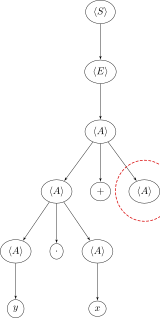
\includegraphics[scale=0.5]{figures/trees/gp_grow_tree_options.pdf}
	\caption{Different options for extending a derivation tree - An unfinished branch consisting of a variable can either be extended by applying a production that includes at least one variable (lower-right tree), or it is ended by inserting a terminal symbol as a leaf (upper-right tree).}
	\label{fig:gp-tree-growing-options}
\end{figure}
The productions available for the variable $\ps{A}$ can be classified into two categories, which we call \emph{terminal} and \emph{non-terminal productions}.
Terminal productions are those that generate subexpressions exclusively consisting of terminal symbols, leading to the creation of one or multiple leaves and, thus, ending the growth of the tree at this particular point, which is illustrated by the upper-right tree in Figure~\ref{fig:gp-tree-growing-options}.
In contrast, non-terminal productions include all those that generate expressions that include at least one variable.
The consequence of applying such a production is that the growth of the tree continues at the respective branch based on the productions available for the generated variables.
This is illustrated by the lower-right tree shown in Figure~\ref{fig:gp-tree-growing-options}. 
We can, therefore, utilize these different types of productions to control the shape of the generated derivation trees within the population initialization.
Two commonly used initialization operators that are based on this observation are the \emph{full} and \emph{grow} operators~\cite{poli2008field}.  
The goal of both operators is to generate a tree that satisfies a certain \emph{depth}, which is defined as the maximum over the length of all paths from the root node to any leaf.
As the name suggests, the \emph{full} operator aims to generate a tree with even depth throughout all branches, which means that every path to a leaf has roughly the same length, for instance, by applying non-terminal productions within each subtree until the necessary depth is reached.
In contrast, the \emph{grow} operator does not impose any constraints on the depth of each path within the tree but instead only requires the longest path to fulfill this condition, which means that both terminal and non-terminal productions are allowed until the depth limit is reached.
Note that in general, a grammar is not required to include both terminal and non-terminal productions for each variable and, hence, the \emph{full} operator can only be applied to a subset of all possible grammars.
In contrast, the \emph{grow} operator is more widely applicable since it only requires a single path within the tree to reach a certain depth, but has the disadvantage that the average shape of the generated trees strongly depends on the ratio of the terminal to non-terminal productions and the arity of the latter, i.e., the number of variables in the generated expressions.
However, this problem can be mitigated by adapting the probability of choosing a production from both categories accordingly. 
Finally, another possibility to initialize the population is to employ both operators, \emph{full} and \emph{grow}, on a certain proportion of the individuals using a variety of different depth limits. 
If the proportion of individuals is roughly 50 \% for both operators, the initialization is called \emph{ramped half-and-half}~\cite{poli2008field,koza1994genetic}.
Furthermore, while both initialization operators presented here can also be applied to other non-grammar-based GP variants, alternative methods specifically designed for G3P have been proposed in~\cite{garcia2006initialization,criado2020grammatically}.
These operators aim to exploit the structure of a given grammar, for instance, in order to generate a population that is more uniformly distributed across the search space~\cite{criado2020grammatically}.

\subsection{Fitness Evaluation and Selection}
\label{sec:gggp-evaluation-and-selection}
Since GGGP is a program optimization technique, each individual corresponds to a program of the form of Equation~\eqref{eq:gp-program}.
However, as the search itself is performed on the genotype representation of each individual, as described in the last section, this representation first needs to be translated to the phenotype, which corresponds to a program in the target language.
In many GGGP program synthesis tasks, the grammar employed within the search is either equivalent or represents a subset of that of the target programming language.
While in such cases a direct correspondence between the derivation and expression tree of the target programming language exists, there is also the possibility to employ multiple layers of intermediate representations before an actual program is generated, which necessitates the implementation of multiple code generation steps.
After an executable program is available in the target language, the final step within fitness evaluation is then to measure its performance in a number of test cases, which is then condensed to one or multiple measure of an individuals fitness, usually each in form of a single numerical value.
For instance, one simple way to assess a program's quality in solving a number of test cases is to represent its performance in each individual test case as a separate optimization objective.
An alternative possibility is to represent different aspects of a program's quality in form of distinct objectives, each of which is determined from a combination of its performance in multiple or even the complete test cases.
With respect to fitness evaluation, GP algorithms can be categorized into single and multi-objective variants.
Similar to other evolutionary algorithms, GP treats fitness evaluation as a block box, which means that its inner workings are independent of the computational details of fitness evaluation, but instead the search is performed exclusively based on the resulting fitness landscape~\cite{pitzer2012comprehensive}.
However, as fitness evaluation often represents the computationally most expensive part of an evolutionary algorithm, it drastically impacts to what extent the given search space can be explored.
Since each individual represents a distinct program that can be executed on a unique set of test instances, each evaluation can be performed independently which facilitates its concurrent execution on a multi-processor system.
For this purpose, parallel~\cite{sudholt2015parallel} and distributed~\cite{gong2015distributed} evolutionary algorithm variants have been proposed, that can be executed on recent manycore architectures and computer clusters.
Due to the inherent similarity of the internal structure of Algorithm~\ref{alg:genetic-programming} to other evolutionary algorithms, these approaches are equally applicable to GP-based search methods. 

After a single or multi-objective fitness value has been assigned to each individual, obtained, the questions remains how the search should be progressed by selecting a number of individuals for the application of the two main evolutionary operators, recombination and mutation.
While initialization aims to generate a population that is evenly spread over the whole search space, the purpose of mutation and recombination is to create novel individuals based on an existing population that are located in a more promising subspace.  
For this purpose, evolutionary algorithms usually employ an additional selection phase to identify promising candidates in the current population based on which these operations are performed, as it outlined in line 4 of Algorithm~\ref{alg:genetic-programming}.
Note that within this process certain individuals can be selected multiple times.
Common operators represent fitness proportionate selection, where individuals are randomly chosen according to a probability equal to their relative fitness value~\cite{lipowski2012roulette}, and tournament selection, where individuals are compared in a tournament-like fashion to identify the fittest among them~\cite{fang2010review}.
In general, selection is independent of the genotype representation of an individual, but depends solely on the objective function of the target optimization problem. 
Consequently, a selection operator is agnostic of the type of evolutionary algorithm it is applied to. 
For this reason, we only briefly discuss selection here and for a more complete treatment of this operation, the reader is referred to one of the following publications:~\cite{back1997handbook,beyer2002evolution,goldberg1991comparative}.
To deal with multi-objective optimization problems, several selection operators have been proposed, about which an overview can be found in~\cite{coello2007evolutionary,deb2011multi,deb2015multi}.
Many of these operators are based on idea of identifying a domination hierarchy between the individuals of the population, whereby an individual is said to dominate another one if it possesses a superior fitness in all of the objectives.
One way to identify such a hierarchy is to employ a non-dominated sorting procedure, which has been, for instance, proposed in~\cite{deb2002fast,deb2013evolutionary}.
The actual selection can then be performed using a dominance-based tournament selection, while additional diversity metrics can be incorporated to decide between non-dominating individuals~\cite{coello2007evolutionary}.
Another recently proposed multi-objective selection operator that is especially geared towards GP problems where the fitness evaluation is performed on multiple test cases, is lexicase selection.
In lexicase selection individuals are selected according their performance in a randomly chosen ordering of the test cases, whereby a decreasing precedence is assigned to each subsequent case. 
For a more detailed description of this operator, the reader is referred to~\cite{helmuth2014solving,la2016epsilon}.
 
\subsection{Mutation and Recombination}
\label{sec:gggp-mutation-and-recombination}
After selecting a number of candidate individuals from the population, mutation and recombination represent two complementary options to extend the current population towards more promising regions of the search space.
\paragraph{Mutation}
The term mutation is usually referred to as the process of altering the genotype of a given individual, usually in a randomized way, with the purpose of creating an individual that, in the best case, has a higher fitness than its predecessor.
Therefore, mutation is usually applied to one individual at a time.
Since the possibilities of alternating an individual depends on its genotype representation, mutation operators need to be customized to the type of evolutionary algorithm employed.
For this purpose, different mutation operators have been proposed for tree-based genotype representations used within GP~\cite{poli2008field,koza1994genetic}.
The most commonly used GP mutation operator is \emph{subtree replacement}, in which a certain branch of an individual is replaced by a randomly generated subtree, which can, for instance, be created using a similar tree-generation operator as within the population initialization~\cite{poli2008field}.
The resulting mutation operator is illustrated in Figure~\ref{fig:gp-replacement-mutation}, again based on derivation trees generated by the example grammar formulated in Equation~\eqref{eq:gp-example-grammar}.
\begin{figure}
	\centering
	\includegraphics[scale=0.5]{figures/trees/subtree_mutation.pdf}
	\caption{Illustration of subtree replacement within a derivation tree.}
	\label{fig:gp-replacement-mutation}
\end{figure}
While subtree replacement has originally been defined for classical GP, it can be easily adapted to GGGP by introducing the additional constraint that branches with a certain variable as their root node can only be replaced by a subtree generated starting from the exact same variable. 
Furthermore, a second mutation operator, which can be directly derived from subtree replacement, is \emph{insertion}.
While in the former the original branch is replaced and, hence, completely evicted from the original tree, insertion only creates a partial subtree at whose end the original subtree is then attached again, which is illustrated in Figure~\ref{fig:gp-insertion-mutation}.
\begin{figure}
	\centering
	\includegraphics[scale=0.5]{figures/trees/subtree_insertion_mutation.pdf}
	\caption{Illustration of subtree insertion within a derivation tree.}
	\label{fig:gp-insertion-mutation}
\end{figure}
In contrast to subtree replacement, whose applicability in the context of GGGP is independent of the grammar, insertion requires the generation of a subtree that includes the root node of the original branch as a child node at which the latter can then be attached.
While both subtree replacement and insertion, depending on the size of the randomly generated subtree, have the potential to drastically change the structure of the original tree, another possibility to alter a given tree is to replace only a single node with one of the same arity, which is called point mutation.
In the context of GGGP, this operation corresponds to exchanging a certain production with a different one that is available for the same variable.
However, for being valid, the newly inserted production needs to generate a sequence of child nodes in which the same variables occur as in the original sequence.
As a consequence, point mutation can only be applied to the subset of productions that fulfills this conditions, which limits its applicability within GGGP-based search algorithms.

\paragraph{Recombination}
While the goal of mutation is to introduce new genetic information into the population, recombination, often also called crossover, aims to combine the genotypes of existing individuals in novel ways, resulting in an individual with improved fitness compared to its predecessors.
In general, recombination operators can be classified into \emph{homologous} and non-homologous ones, whereby those from the former category preserve the position of the individual elements of the genome.
A straightforward way to perform recombination in tree-based GP is to exchange subtrees between two individuals at a certain (crossover) point within both trees, which is called \emph{subtree crossover}.
Again, to apply this operator within GGGP, the crossover point must be chosen in a way that the root nodes of the exchanged trees correspond to the same variable.
The resulting operation is illustrated in Figure~\ref{fig:gp-subtree-crossover}.  
%TODO include figure
\begin{figure}
	\centering
	\includegraphics[scale=0.5]{figures/trees/subtree_crossover.pdf}
	\caption{Illustration of subtree crossover within a derivation tree.}
	\label{fig:gp-subtree-crossover}
\end{figure}
As subtree crossover permits the exchange of arbitrary subtrees with matching root nodes between two individuals, this operator is non-homologous.
To obtain a similarly functioning homologous recombination operator, one-point crossover has been proposed~\cite{poli1998schema}.
One-point crossover first aligns both trees by traversing them recursively until there occurs a mismatch between the arity of two non-terminal nodes of both trees at the same position.
The crossover point is then chosen from all positions in both trees where such a mismatch occurs and the subtree exchange is performed in a similar way as in subtree crossover.
While this operator preserves the relative position of each node within both trees, only a limited number of crossover points can be selected.
For instance, the subtree exchange shown in Figure~\ref{fig:gp-subtree-crossover} is not a valid single-point crossover operation, as the first arity mismatch already occurs above the chosen crossover point within the respective branches of both trees.
In general, the applicability of single-point crossover within a GGGP system depends on the amount of productions available for each variable within the grammar.
In particular, if the majority of productions generates only a single variable, the average derivation tree possesses a small branching factor and, therefore, the number of possible crossover points for performing single-point crossover is low.
Finally, it must be mentioned that, besides the ones discussed here, a variety of different mutation and crossover operators have been proposed since the invention of GP, of which an overview can be found in~\cite{poli2008field}.
Furthermore, since these operators are designed for general tree-based GP systems and, hence, when applied in a GGGP setting do not take the underlying grammatical representation into account, in~\cite{couchet2007crossover} mutation and crossover operators that are tailored towards GGGP have been proposed. 

After creating a number of novel individuals by means of mutation and crossover, the remaining questions that needs to be addressed is how the search should be progressed by assembling a new population from the combined set of the newly created ones and those from the previous generation, as illustrated in line 7 Algorithm~\ref{alg:genetic-programming}.
Here one possibility is to completely replace the previous generation by the individual created by the mentioned genetic operators.
However, this approach incurs the danger of evicting individuals that are located in promising areas the search space, which then need to be rediscovered later in order to continue the search at this point.
Therefore, many evolutionary algorithms employ \emph{elitism}, which means that individuals from the previous population are allowed to pass over to the next one in case their fitness is not surpassed by enough newly created individuals.
While the application of elitism prevents the occurrence of fitness regressions from one generation to the next, it comprises the danger of getting stuck in local optima.
For this purpose, the amount of elitism always represents a compromise between the loss of promising individuals and the danger of premature convergence to local optima.
Options to mitigate this risk and prevent locally-optimal individuals from quickly overtaking the population are, for instance, to restrict the amount of elitism to only a subset of the population and to introduce additional niching or diversity criteria into to process of selecting individuals for the next population, which is especially common in multi-objective evolutionary algorithms~\cite{coello2007evolutionary}.
\chapter{A Formal Language for Multigrid Methods}
\label{chapter:multigrid-formal-language}
  \section{Context-Free Multigrid Construction Rules}
\chapter{The EvoStencils Framework - Part 1: Core Implementation}
\label{chapter:evostencils-1}
  \usemintedstyle{tango}
\setminted[python]{fontsize=\footnotesize}
In the first part of this thesis we have established a theoretical basis about multigrid methods, formal languages and genetic programming.
In Chapter~\ref{chapter:multigrid-formal-language}, building on this foundation, we have then developed a novel formal language and grammar for the automatic generation of multigrid methods. 
While we have already demonstrated that the capabilities of this approach in alternating each individual step of a multigrid method, we could not yet demonstrate its benefits compared to the use of classical multigrid cycles, such as V-, F- and W-cycles.
We aim to achieve this goal with the implementation of \emph{EvoStencils}, a prototypical Python framework for the grammar-guided optimization of multigrid methods.
Using this framework we will then show how it is possible to evolve methods that are more efficient than all common multigrid cycles in solving a number of PDE-based problems while being structurally different that any other known method of this type.
However, before we discuss EvoStencils' features and their implementation in Python, we want to provide an overview about its workflow and software architecture.
In general, we can distinguish between EvoStencils' core implementation and the functionality of the framework that is build upon the use of external libraries.
First of all, since our formulation of the rules to construct a multigrid methods in the form of a context-free grammar, we can utilize the grammar-guided genetic programming techniques presented Chapter~\ref{chapter:formal-languages-and-gp} without adapting their inner workings.
For this purpose, we employ the widely-used evolutionary computation framework DEAP\footnote{DEAP: \url{https://github.com/deap/deap}}~\cite{rainville2012deap}, which enables us to implement GGGP in a modular way while requiring only a limited amount of adaption.
However, the questions that then remains to be answered how we can evaluate each multigrid method obtained through GGGP in an automatic and reproducible manner.
As we have seen in Section~\ref{sec:grammar-based-algorithm-generation} the 

\begin{figure}
	\resizebox{\columnwidth}{!}{%
		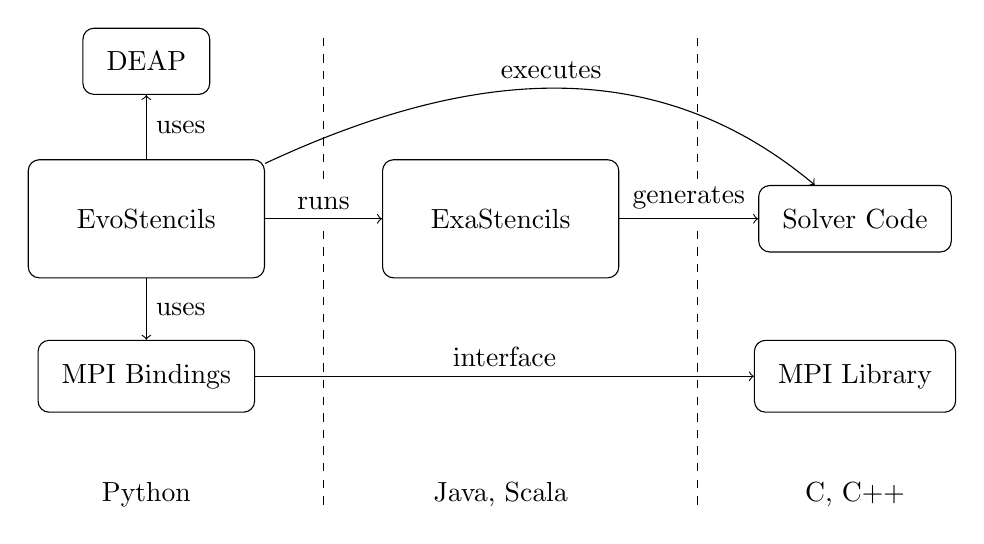
\begin{tikzpicture}
			%\draw [help lines] (-10,-10) grid (10,10);
			\node[draw, minimum width=3cm, minimum height=1.5cm, rounded corners] (evo) at (0,0) {EvoStencils};
			\node[draw, inner sep=3mm, rounded corners] (bindings) at (0, -2) {MPI Bindings};
			\node[draw, inner sep=3mm, rounded corners] (deap) at (0, 2) {DEAP};
			\node[draw, minimum width=3cm, minimum height=1.5cm, rounded corners] (exa) at (4.5, 0) {ExaStencils};
			\node[draw, inner sep=3mm, rounded corners] (code) at (9, 0) {Solver Code};
			\node[draw, inner sep=3mm, rounded corners] (mpi) at (9, -2) {MPI Library};
			\draw[dashed] (2.25, 2.3) -- (2.25,0.5);
			\draw[dashed] (2.25, -0.15) -- (2.25,-3.7);
			\draw[dashed] (7, 2.3) -- (7,0.5);
			\draw[dashed] (7, -0.15) -- (7,-3.7);
			\node (python) at (0, -3.5) {Python};
			\node (java) at (4.5, -3.5) {Java, Scala};
			\node (c) at (9, -3.5) {C, C++};
			\draw[->] (evo)-- node[anchor=west] {uses} (deap);
			\draw[->] (evo)-- node[anchor=south]{runs} (exa);
			\draw[->] (exa)--node[anchor=south] {generates} (code);
			\draw[->] (evo) to [out=25,in=140] node[anchor=south] {executes} (code);
			\draw[->] (bindings)--node[anchor=south] {interface}(mpi);
			\draw[->] (evo)--node[anchor=west] {uses}(bindings);
			%\draw[->] (mpi)--(code);
		\end{tikzpicture}
	}\caption{Software Architecture of EvoStencils.}
	\label{fig:evostencils-architecture}
\end{figure}

\begin{listing}
	\inputminted{python}{evostencils/ir/grid.py}
	\caption{Class for Representing Uniform Grids}
\end{listing}
\begin{listing}
	\inputminted{python}{evostencils/ir/expression.py}
	\caption{Abstract Expression Base Class}
\end{listing}
\begin{listing}
	\inputminted{python}{evostencils/ir/entity.py}
	\caption{Base Class for Representing Entities}
\end{listing}
\begin{listing}
	\inputminted{python}{evostencils/ir/unary_expression.py}
	\caption{Base Class for Representing Unary Expressions}
\end{listing}
\begin{listing}
	\inputminted{python}{evostencils/ir/binary_expression.py}
	\caption{Base Class for Representing Binary Expressions}
\end{listing}
  \label{chapter:evostencils-2}
\chapter{The EvoStencils Framework - Part 2: Generalization and Parallelization}
  \section{Block Smoothers}
\section{Systems of Partial Differential Equations}
\section{Distributed Parallelization}
\chapter{Experiments and Discussion}
\label{chapter:experiments}
  As a first step in the evaluation of our evolutionary program synthesis method, we consider two PDE-based model problems, Poisson's equation and a linear elastic boundary value problem, which can already be solved efficiently by applying common multigrid cycles iteratively.
Here, our goal is, first of all, to demonstrate that our approach is able to reliably find functioning multigrid cycles in a number of randomized independent experiments.
Furthermore, since the known multigrid cycles already provide a strong baseline for these problems, we can investigate whether the methods designed with our approach are able to achieve a similar degree of efficiency.
In addition, by considering both two- and three-dimensional problems as well as a system of PDEs, we can demonstrate that our implementation is able to handle PDEs of different types.
\section{Automating the Design of Multigrid Cycles for Common PDEs}
\label{sec:experiments-part1}
As it has been mentioned above, the goal of this section is to evaluate the effectiveness of our evolutionary program synthesis method for the automated design of multigrid cycles that are able to quickly reduce the error of a given discretized PDE.
Therefore, the problem instances considered in this section are chosen in a way that facilitates their efficient solution by multigrid.
This is reflected in the fact that common multigrid cycles, as described in Section~\ref{sec:multigrid-cycles}, are able to quickly converge to the correct solution of each of the resulting systems of linear equations.
We begin this section by introducing the considered problem instances and their mathematical formulation.
At this point, we want to emphasize that all results presented in this section have been originally published as part of the paper~\cite{schmitt2021evostencils}.
However, this thesis complements this work with an additional analysis of the multigrid solvers obtained by our evolutionary search method.
\subsection{Problem Formulation}
\subsubsection{Poisson's Equation}
\label{sec:poisson-equation}
Poisson's equation is an elliptic PDE that occurs in the study of many physical phenomena~\cite{folland2020introduction} and is defined as
\begin{equation}
	\begin{split}
		-\nabla^{2} u & = f \quad \text{in} \; \Omega \\
		u & = g \quad \text{on} \; \partial \Omega.
	\end{split}
	\label{eq:poisson}
\end{equation}
In our experimental evaluation, we consider two different instances of Poisson's equation with Dirichlet boundary conditions, which are summarized in Table~\ref{table:poisson-problems}.
\begin{table}
	\begin{tabular}{r l l}
		\toprule
		Problem & 2D Poisson & 3D Poisson \\
		\midrule
		$\Omega = $ & $ (0, 1)^2$ & $(0, 1)^3$ \\
		\midrule
		$f(\bm{x}) = $ & $\pi^2 \cos(\pi x) - 4 \pi^2 \sin(2 \pi y)$ & $x^2 - 0.5 y^2 - 0.5 z^2$ \\
		\midrule
		$g(\bm{x}) = $ & $\cos(\pi x) - \sin(\pi y)$ & $0$ \\
		\bottomrule
	\end{tabular}
	\caption{Poisson problem instances.}
	\label{table:poisson-problems}
\end{table}
Note that in Section~\ref{sec:execution-time-analysis}, we have employed the same two-dimensional instance of Poisson's equation to estimate the relative cost of each operation within our evolutionary search method.
We discretize the Laplace operator $\nabla^{2}$ with finite differences on a uniform cartesian grid with step size $h = 1/2^{l_{max}}$, which yields the five-point stencil
\begin{equation*}
	\nabla^2_h = 
	\frac{1}{h^2} \begin{bmatrix}
		0 & 1 & 0\\
		1 & -4 & 1 \\
		0 & 1 & 0  
	\end{bmatrix},
\end{equation*}
in two dimensions, and the seven-point stencil
\begin{equation*}
\nabla^2_h = 
\frac{1}{h^2} \begin{bmatrix}
	\begin{bmatrix}
	0 & 0 & 0 \\
	0 & 1 & 0 \\
	0 & 0 & 0
	\end{bmatrix}
	&		
	\begin{bmatrix}
	0 & 1 & 0 \\
	1 & -6 & 1 \\
	0 & 1 & 0 
	\end{bmatrix} &
	\begin{bmatrix}
	0 & 0 & 0 \\
	0 & 1 & 0 \\
	0 & 0 & 0
\end{bmatrix}
\end{bmatrix}
\end{equation*} in three dimensions.
We choose a maximum level of $l_{max} = 11$ in 2D and $l_{max} = 7$ in 3D, which results in systems of linear equations consisting of $4\,190\,209$ and $2\,048\,383$ unknowns, respectively.

\subsubsection{Linear Elasticity}
Linear elasticity is a fundamental branch of solid mechanics with numerous applications in engineering and material science~\cite{holzapfel2001nonlinear}.
It is derived from the more general theory of nonlinear continuum mechanics by assuming a linear relationship between stress and strain during elastic deformation.
We consider a two-dimensional linear elastic boundary value problem given by the system of PDEs
\begin{equation}
	\begin{split}
		(\alpha + \beta) \cdot (\frac{\partial^2}{\partial x^2} u + \frac{\partial^2}{\partial x \partial y} v) + \alpha \nabla^2 u & = 0 \quad \text{in} \; \Omega \\
		(\alpha + \beta) \cdot (\frac{\partial^2}{\partial x \partial y} u + \frac{\partial^2}{\partial y^2} v) + \alpha \nabla^2 v & = 0 \quad \text{in} \; \Omega \\
		u = 0 \quad \text{and} \quad v & = g \quad \text{on} \; \partial \Omega 
		\label{eq:linear-elasticity}
	\end{split}
\end{equation}
where $\Omega = (0,1)^2$, $\alpha = 195$, $\beta = 130$ and
\begin{equation*}
	g(x,y) = 0.4 \, (1 - x) \, x y \, \sin(\pi x).
\end{equation*}
From a physical point of view, this system can be interpreted as a two-dimensional rectangular body that undergoes an elastic deformation into the y-direction, as it can be seen in Figure~\ref{fig:visualization-linear-elasticity}.
\begin{figure}
	\centering
	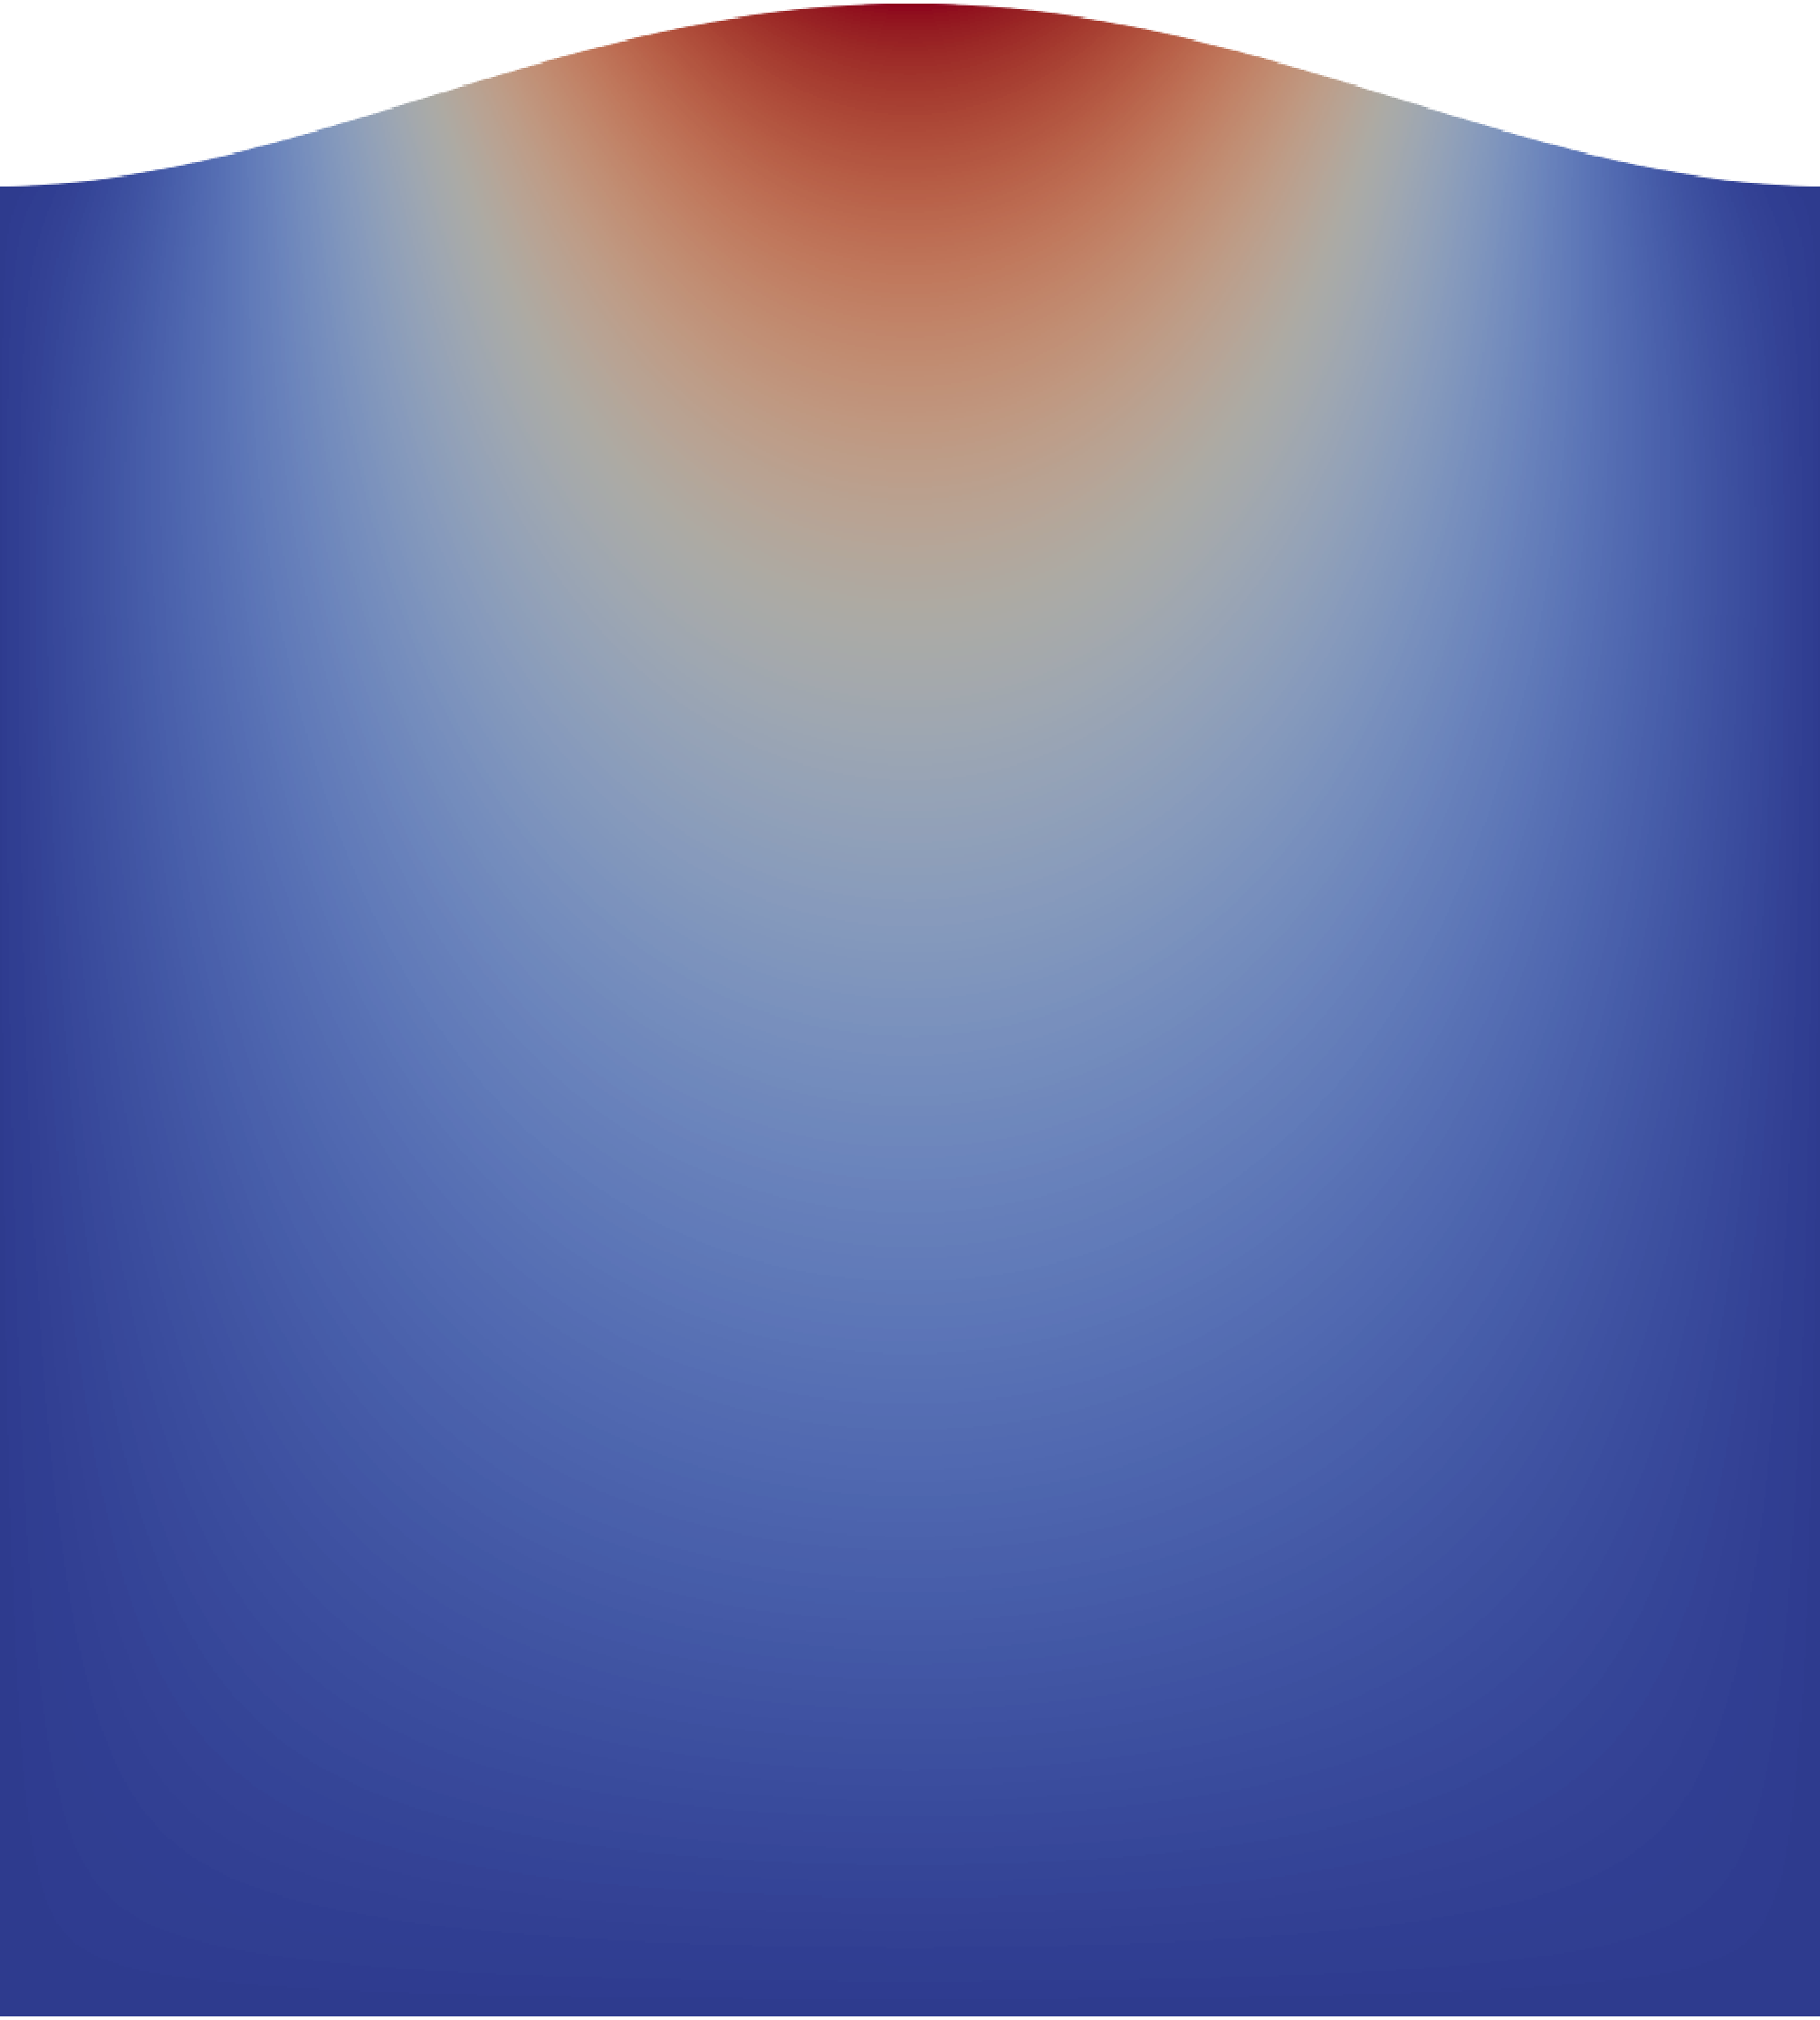
\includegraphics[width=0.5\textwidth]{figures/visualization-linear-elasticity1}
	\caption{Visualization of the considered linear elastic boundary value problem. A two-dimensional rectangular body undergoes an elastic deformation into the y-direction.}
	\label{fig:visualization-linear-elasticity}
\end{figure}
We discretize Equation \eqref{eq:linear-elasticity} with finite differences on a cartesian grid using a step size $h = 1/2^{l_{max}}$ with $l_{max} = 10$, which yields a system of linear equations $\bm{A} \bm{u} = \bm{f}$ with 
\begin{equation*}
	\bm{A} =
	\begin{pmatrix}
		(\alpha + \beta) \frac{\partial^2}{\partial x^2} + \alpha \nabla^2 & (\alpha + \beta) \frac{\partial^2}{\partial x \partial y} \\
		(\alpha + \beta) \frac{\partial^2}{\partial x \partial y} & (\alpha + \beta) \frac{\partial^2}{\partial y^2} +  \alpha \nabla^2
	\end{pmatrix},
\end{equation*}
\begin{equation*}
	\bm{u} = \begin{pmatrix}
		u \\ v
	\end{pmatrix}, \quad
	\bm{f} =
	\begin{pmatrix}
		f_{u} \\ f_{v}
	\end{pmatrix} =
	\begin{pmatrix}
		0 \\ 0
	\end{pmatrix},
\end{equation*}
whereby the differential operators $\nabla^2$, $\frac{\partial^2}{\partial x^2}$, $\frac{\partial^2}{\partial y^2}$ and $\frac{\partial^2}{\partial x \partial y}$ are approximated by their discrete counterparts
\begin{equation*}
	\left(\nabla^2 u\right)_{i,j} = 
	\frac{1}{h^2} \begin{bmatrix}
		0 & 1 & 0\\
		1 & -4 & 1 \\
		0 & 1 & 0  
	\end{bmatrix},
\end{equation*}
\begin{equation*}
	\left(\frac{\partial^2}{\partial x^2} u\right)_{i,j} =
		\frac{1}{h^2} \begin{bmatrix}
		0 & 0 & 0\\
		1 & -2 & 1 \\
		0 & 0 & 0  
	\end{bmatrix},
\end{equation*}
\begin{equation*}
	\left(\frac{\partial^2}{\partial y^2} u\right)_{i,j} =
	\frac{1}{h^2} \begin{bmatrix}
		0 & 1 & 0\\
		0 & -2 & 0 \\
		0 & 1 & 0  
	\end{bmatrix},
\end{equation*}
\begin{equation*}
	\left(\frac{\partial^2}{\partial x \partial y} u\right)_{i,j} = 
	\frac{1}{4 h^2} \begin{bmatrix}
		-1 & 0 & 1\\
		0 & 0 & 0 \\
		1 & 0 & -1  
	\end{bmatrix}.
\end{equation*}
Similar to the above case, we employ a uniform cartesian grid with a step size $h = 1/2^{l_{max}}$ with $l_{max} = 10$, such that the resulting system of linear equations contains $2\,093\,058$ unknowns.
\subsection{Multigrid Configuration}
\label{sec:experiments1-multigrid-configuration}
To design an efficient multigrid method, we consider each of the given problems on a grid hierarchy consisting of five discretization levels $l \in \left[l_{max} - 4, l_{max}\right]$, where the grid spacing on each level is given by the formula $h = 1/2^l$.
We then obtain the respective operator on each level by applying the same discretization method as on the finest grid.
Therefore, the resulting grammar is structurally similar to the one shown in Table~\ref{table:multigrid-grammar}.
Within each grammar production rule, we consider the following components:
\begin{description}
	\item[\textbf{Smoothers}:] Decoupled / Collective Jacobi and red-black Gauss-Seidel (RB-GS), block Jacobi with rectangular blocks up to a maximum number of six terms~\cite{trottenberg2000multigrid}.
	\item[\textbf{Restriction}:] Full-weighting restriction.
	\item[\textbf{Prolongation}:] Bilinear interpolation.
	\item[\textbf{Relaxation factors}:] $\omega \in \left( 0.1 + 0.05i \right)_{i = 0}^{36} = \left(0.1, 0.15, 0.2, \dots, 1.9 \right)$
	\item[\textbf{Coarse-grid solver}:] Conjugate gradient method for $l = l_{max} - 4$.
\end{description}
Here, we generate block Jacobi smoothers by defining a splitting $A = L + D + U$ where $D$ is a block diagonal matrix of the form
\begin{equation*}
	D = 
		\begin{pmatrix}A_{11}&0&\cdots &0\\
			0&A_{22}&\cdots &0\\
			\vdots &\vdots &\ddots &\vdots \\0&0&\cdots &A_{mm}\end{pmatrix},
\end{equation*}
where each matrix $A_{ij}$ corresponds to a set of adjacent grid points contained in the respective rectangular block, as it has been discussed in Section~\ref{subsec:block-smoothing}.
A more detailed treatment of block relaxation methods can be found in~\cite{trottenberg2000multigrid}.
For each smoothing and coarse-grid correction step, the relaxation factor $\omega$ can be chosen from the above interval.
As a baseline for assessing the efficiency and generalizability of the designed multigrid solvers, we consider a number of common multigrid cycles with RB-GS smoothing and optimized relaxation factors.
We, therefore, formulate these methods on the same five-grid hierarchy using the same restriction, prolongation operators, and coarse-grid solver.
In each case, we consider the corresponding linear system as solved when the initial residual has been reduced by a factor of $10^{-12}$.

\subsection{Experimental Settings and Evaluation Platform}
\label{sec:optimization-settings}
After specifying the operator and parameter choices considered within the construction of each multigrid solver, we next describe the settings under which we perform each experiment.
Here, we utilize the EvoStencils framework, whose implementation has been described in detail in Chapter~\ref{chapter:evostencils-1} and~\ref{chapter:evostencils-2}.
The goal of each experiment is to evolve a set of non-dominated individuals according to the two objectives convergence factor $\rho$ and execution time per iteration $t$, as described in Section~\ref{sec:fitness-evaluation-and-selection}, which are evaluated by applying each multigrid cycle as an iterative solver to the respective test problem.
The resulting individuals are then subject to a subsequent evaluation and comparison with the available reference methods. 
Table~\ref{table:gp-parameters} gives an overview of the algorithmic configuration used within each experiment.
\begin{table}
	\centering
	\caption{Summary of G3P configuration parameters.}
	\label{table:gp-parameters}
	\begin{tabular}{l c}
		\toprule
		Parameter & Value \\
		\midrule 
		Evolutionary algorithm type & $(\mu + \lambda)$ \\
		\midrule
		Objectives & $t, \rho$ \\
		\midrule
		Number of generations & 250 \\
		\midrule
		Initial population size & 2048 \\
		\midrule
		$\lambda$ & 256 \\
		\midrule
		$\mu$ & 256 \\
		\midrule
		Number of MPI processes & 64 \\
		\midrule
		Non-dominated sorting procedure & \cite{deb2002fast} \\ 
		\midrule
		Selection operator & \cite{deb2002fast} \\ 
		\midrule
		Crossover operator & Single-point crossover \\
		\midrule
		Crossover probability & $2/3$ \\
		\midrule
		Mutation operator & Random subtree insertion \\
		\midrule 
		Probability to mutate a terminal symbol & $1/3$ \\
		\bottomrule
	\end{tabular}
\end{table}
Within each run, starting with a randomly generated population of 2048 individuals, we perform an evolutionary search for 250 generations.
In each generation, we create new individuals by first selecting $\lambda = 256$ candidates from the current population.
We then apply mutation and crossover to each pair of selected candidates to create two child individuals, whereby the crossover probability is set to $2/3$, and in case of mutation, we choose a terminal symbol with a probability of $1/3$.
As a mutation operator, we employ subtree insertion whenever possible. Otherwise, the respective subtree is completely replaced by a randomly-created one, as described in Section~\ref{sec:gggp-mutation-and-recombination}.
The resulting individuals are then evaluated according to the two objectives by generating a parallel C++ solver implementation using the ExaStencils framework, which is applied to the respective problem as described above.
Hereby we distribute the evaluation of all 256 individuals to 64 MPI processes, such that each process is responsible for the evaluation of four individuals.
The resulting fitness values are distributed to all 64 processes, such that each of them possesses an identical copy of each child individual together with its fitness value, as it has been described in Chapter~\ref{sec:distributed-parallelization}.
Finally, we select $\mu = 256$ individuals as a population for the next generation from the combined set of parent and child individuals using the NSGA-II non-dominated sorting procedure~\cite{deb2002fast}.

As an evaluation platform for running each experiment, we employ 32 nodes of the Meggie compute cluster of the Erlangen National High-Performance Computing Center (NHR), where each node of the system consists of two sockets, each with ten physical CPU cores.
Therefore, each process is pinned and executed on a dedicated socket, while for the evaluation of each solver, we employ a thread-based parallelization using ten OpenMP threads, whereby each tread is pinned to a distinct physical compute core on the respective socket.
For the parallelization of each nested loop, we employ static scheduling based on the outer-loop range, such that each thread processes a consecutive chunk of iterations.
To generate a thread-parallel executable for each solver, we employ the GCC 9.3.0 compiler with the -O3 optimization level.
To reduce statistical variations between individual evaluation runs, we execute each solver three times and then compute the average for both objectives.

\subsection{Algorithm Behavior Analysis}
\label{sec:experiments1-algorithm-behavior-analysis}
As a first step towards a quantitative evaluation of our evolutionary program synthesis method, we assess whether our algorithm is able to effectively find good solutions with respect to our two optimization objectives.
For this purpose, we measure the minimum of each of the two objectives within the population throughout each of the ten experiments for all three test problems.
As a result, Figure~\ref{fig:poisson-2D-minimum-objectives},~\ref{fig:poisson-3D-minimum-objectives} and~\ref{fig:linear-elasticity-2D-minimum-objectives} shows the mean and standard deviation of the current optimum of both objectives over all experiments.
\begin{figure}
	\centering
	\begin{subfigure}[b]{0.49\textwidth}
		\centering
		\includegraphics[width=\textwidth]{figures/minimum_convergence_factor_2D_FD_Poisson_fromL2.pdf}
		\caption{Minimum Convergence Factor}
		\label{fig:poisson-2D-minimum-convergence-factor}
	\end{subfigure}
	\hfill
	\begin{subfigure}[b]{0.49\textwidth}
		\centering
		\includegraphics[width=\textwidth]{figures/minimum_execution_time_2D_FD_Poisson_fromL2.pdf}
		\caption{Minimum Execution Time per Iteration}
		\label{fig:poisson-2D-minimum-execution-time}
	\end{subfigure}
	\caption{2D Poisson - Mean and standard deviation of the minimum objective function values during the optimization.}
	\label{fig:poisson-2D-minimum-objectives}
\end{figure}
\begin{figure}
	\centering
	\begin{subfigure}[b]{0.49\textwidth}
		\centering
		\includegraphics[width=\textwidth]{figures/minimum_convergence_factor_3D_FD_Poisson_fromL2.pdf}
		\caption{Minimum Convergence Factor}
		\label{fig:poisson-3D-minimum-convergence-factor}
	\end{subfigure}
	\hfill
	\begin{subfigure}[b]{0.49\textwidth}
		\centering
		\includegraphics[width=\textwidth]{figures/minimum_execution_time_3D_FD_Poisson_fromL2.pdf}
		\caption{Minimum Execution Time per Iteration}
		\label{fig:poisson-3D-minimum-execution-time}
	\end{subfigure}
	\caption{3D Poisson - Mean and standard deviation of the minimum objective function values during the optimization.}
	\label{fig:poisson-3D-minimum-objectives}
\end{figure}
\begin{figure}
	\centering
	\begin{subfigure}[b]{0.49\textwidth}
		\centering
		\includegraphics[width=\textwidth]{figures/minimum_convergence_factor_2D_FD_LinearElasticity_fromL2.pdf}
		\caption{Minimum Convergence Factor}
		\label{fig:linear-elasticity-2D-minimum-convergence-factor}
	\end{subfigure}
	\hfill
	\begin{subfigure}[b]{0.49\textwidth}
		\centering
		\includegraphics[width=\textwidth]{figures/minimum_execution_time_2D_FD_LinearElasticity_fromL2.pdf}
		\caption{Minimum Execution Time per Iteration}
		\label{fig:linear-elasticity-2D-minimum-execution-time}
	\end{subfigure}
	\caption{2D Linear Elasticity - Mean and standard deviation of the minimum objective function values during the optimization.}
	\label{fig:linear-elasticity-2D-minimum-objectives}
\end{figure}
First of all, we can conclude that in all three cases, our algorithm is able to quickly reduce the minimum value of both objectives within the population.
If we compare the slope of the two objectives for the three different problems, we can see that in the case of the first objective $\rho$, significantly more generations are required to achieve the same degree of reduction as for the second objective $t$.
However, the algorithm still significantly improves upon the current minimum of $\rho$ beyond the first 50 generations, which can be seen in Figure~\ref{fig:poisson-2D-minimum-convergence-factor},~\ref{fig:poisson-3D-minimum-convergence-factor} and~\ref{fig:linear-elasticity-2D-minimum-convergence-factor}.
For the second objective $t$, the majority of improvement happens within the first 50--70 generations, as it can be seen in Figure~\ref{fig:poisson-2D-minimum-execution-time},~\ref{fig:poisson-3D-minimum-execution-time} and~\ref{fig:linear-elasticity-2D-minimum-execution-time}.
Note that while the convergence factor is constant for each execution of the same solver, $t$ is obtained by measuring its execution time on the respective compute node.
Therefore, due to manufacturing and temperature-based variations, we can expect a certain degree of fluctuations when measuring the execution time of the same solver on different compute nodes during consecutive optimization runs.
Consequently, even though the algorithm is able to reduce the second objective faster, this effect induces a larger deviation between the individual experiments and, thus, an overall higher standard deviation.

Furthermore, by considering the absolute value of the minimum convergence factor attained in each of the three different cases, we can assess the difficulty of the underlying problem.
While the execution time per iteration $t$ is solely determined by the computational complexity of each solver and the properties of the given computer architecture, a smaller convergence factor indicates that the underlying problem is easier to solve.
Poisson's equation represents an often-studied model problem whose strong ellipticity enables its easy solution by multigrid~\cite{trottenberg2000multigrid}.
As a consequence, our method consistently discovers multigrid methods that achieve fast convergence, with minimum convergence factors of less than 0.005, for both the two and three-dimensional instances of this equation, which can be seen in Figure~\ref{fig:poisson-2D-minimum-convergence-factor} and~\ref{fig:poisson-3D-minimum-convergence-factor}.
In the case of the linear elastic boundary value problem, both the mean and standard deviation remain higher for the first objective throughout each experiment.
However, on average, our method is still able to discover multigrid methods that achieve a convergence factor of 0.01 or less, which equates to outstandingly fast convergence.
In summary, we can conclude that our evolutionary program synthesis method consistently yields multigrid cycles that represent satisfactory minima for both objectives in all three test cases considered.

To further analyze the behavior of our multi-objective evolutionary algorithm, we consider the distribution of non-dominated individuals at the end of all experiments, which is shown in Figure~\ref{fig:pareto-front-2D-poisson},~\ref{fig:pareto-front-3D-poisson} and~\ref{fig:pareto-front-2D-linear-elasticity}.
\begin{figure}
	\includegraphics[width=\columnwidth]{figures/pareto_front_2D_FD_Poisson_fromL2.pdf}
	\caption{2D Poisson - Distribution of non-dominated individuals at the end of all ten experiments. The red line denotes the combined Pareto front.}
	\label{fig:pareto-front-2D-poisson}
\end{figure}
\begin{figure}
	\includegraphics[width=\columnwidth]{figures/pareto_front_3D_FD_Poisson_fromL2.pdf}
	\caption{3D Poisson - Distribution of non-dominated individuals at the end of all ten experiments. The red line denotes the combined Pareto front.}
	\label{fig:pareto-front-3D-poisson}
\end{figure}
\begin{figure}
	\includegraphics[width=\columnwidth]{figures/pareto_front_2D_FD_LinearElasticity_fromL2.pdf}
	\caption{2D Linear Elasticity - Distribution of non-dominated individuals at the end of all ten experiments. The red line denotes the combined Pareto front.}
	\label{fig:pareto-front-2D-linear-elasticity}
\end{figure}
Here the red line denotes the combined front, while the color density of the distribution indicates where most of the solutions are located at the end of all experiments. 
In all three cases, the majority of non-dominated solutions obtained within each experiment can be found close to the combined front.
While in Figure~\ref{fig:pareto-front-2D-poisson}, the number of solutions that are distinctly located outside of the front is slightly higher than in the other two cases, their distance to the red line is still comparably small compared to the complete objective space.
Again we can attribute part of this effect to variations in the execution time on different compute nodes.
Furthermore, note that throughout most of the objective space, but especially in the center, the solutions are evenly distributed alongside the front.
Here only the left-upper part of Figure~\ref{fig:pareto-front-3D-poisson} and~\ref{fig:pareto-front-2D-linear-elasticity} represents a noteworthy exception, where our approach struggles to discover the same solutions within each experiment.
An explanation for this effect is that the solutions located in this part of the space are characterized by an extremely fast convergence.
Since the convergence of a multigrid method can primarily be accelerated with the addition of smoothing and coarse-grid correction steps, discovering the same non-dominated solutions with fast convergence requires us to construct the same large expressions starting from different random initializations.
Recently, the impaired capabilities of NSGA-II to evolve large non-dominated expressions have been demonstrated in~\cite{liu2022evolvability}, which similarly explains why our implementation struggles to consistently discover the same fast-converging solutions.

\subsection{Comparison with Reference Methods}
Finally, in order to investigate whether our evolutionary program synthesis method yields multigrid methods that are competitive with well-known multigrid cycles, we consider two different multi-core CPU architectures for evaluation: Intel Xeon E5-2630v4 (Broadwell) and Intel Xeon 2660v2 (Ivy Bridge).
In both cases, each compute node consists of two sockets with 20 physical CPU cores and a cache-coherent NUMA architecture.
In order to assess the solving speed of the methods evolved, we consider two different problem sizes for each of the three test cases.
While in the first case, a problem size identical to the one employed within the evolutionary search is chosen, in the second case, we obtain a larger one by doubling the number of grid points in each dimension.
To measure the solving speed of each method, we execute it on a dedicated node using a thread-based parallelization with 20 OpenMP threads, whereby we pin each thread to a unique physical core and employ the same parallelization approach as described in Section~\ref{sec:optimization-settings}.
Even though the evaluation of generalizability is not the focus of this section, it is still worthwhile to investigate whether the methods discovered with our approach are capable of solving larger instances of the same problem.
For comparison, we consider a number of different V-cycles with at most four RB-GS pre and post-smoothing steps.
With the exception of full-multigrid (FMG) methods, which require a different formulation than the one considered here, these cycles are known to be the fastest multigrid-based solvers for Poisson's equation~\cite{trottenberg2000multigrid}.
As we have already investigated in~\cite{schmitt2020constructing}, the same is true for the linear elastic boundary value problem considered here.
To achieve a fair comparison, we empirically choose the optimum relaxation factor $\omega$ for each test case from the same interval considered within our experiments, which leads to $\omega = 1.15$ for the two-dimensional Poisson equation and $\omega = 1.25$ both for the three-dimensional Poisson equation and the linear elastic boundary value problem.
Table~\ref{table:poisson-2D-reference-methods},~\ref{table:poisson-3D-reference-methods} and~\ref{table:linear-elasticity-2D-reference-methods} contains the resulting solving times and the number of iterations required to achieve the desired defect reduction for the respective test case.
Here, for instance, the abbreviation V(2,1) denotes a V-cycle with two pre and one post-smoothing step with RB-GS.
First of all, as we can expect from a functioning multigrid method, the number of iterations stays constant for both problem sizes, only with the exception of the V(1,0)-cycle, where we can observe a slight increase for the linear elastic boundary value problem.
Overall, we can conclude that while the V(2,2)-cycle represents the fastest solver for both cases of Poisson's equation, the V(3,3) cycle leads to the fastest solving time for the linear elastic boundary value problem.
\begin{table}
	\caption{2D Poisson - Measured number of iterations and solving times of the reference methods on 20 cores and two sockets.}
	\label{table:poisson-2D-reference-methods}
	\centering
	\begin{tabular}{l c c c c c c}
		\toprule
		& \multicolumn{2}{c}{Iterations} & \multicolumn{2}{c}{Broadwell (ms)} & \multicolumn{2}{c}{Ivy Bridge (ms)} \\
		\cmidrule(r){2-3} \cmidrule(r){4-5} \cmidrule(r){6-7}
		$l_{max}$ & $11$& $12$ & $11$ & $12$ & $11$ & $12$\\
		\midrule
		V(1, 0) & 21 & 21 & 969 & 2810 & 879 & 2652 \\
		\midrule
		V(1, 1) & 9 & 9 & 461 & 1359 & 411 & 1287 \\
		\midrule
		V(2, 1) & 7 & 7 & 377 & 1137 & 334 & 1087\\
		\midrule
		V(2, 2) & 6 & 6 & 344 & 1056 & 302 & 1007 \\
		\midrule
		V(3, 2) & 6 & 6 & 378 & 1160 & 324 & 1112 \\
		\midrule
		V(3, 3) & 6 & 6 & 397 & 1255 & 344 & 1201 \\
		\midrule
		V(4, 3) & 6 & 6 & 425 & 1350 & 366 & 1306 \\
		\midrule
		V(4, 4) & 6 & 6 & 448 & 1449 & 383 & 1409\\
		\bottomrule
	\end{tabular}
	%FMG for max_level = 12: 530.3038500000001 ms, 3 Iterations
\end{table}
\begin{table}
	\caption{3D Poisson - Measured number of iterations and solving times of the reference methods on 20 cores and two sockets.}
	\label{table:poisson-3D-reference-methods}
	\centering
	\begin{tabular}{l c c c c c c}
		\toprule
		& \multicolumn{2}{c}{Iterations} & \multicolumn{2}{c}{Broadwell (ms)} & \multicolumn{2}{c}{Ivy Bridge (ms)} \\
		\cmidrule(r){2-3} \cmidrule(r){4-5} \cmidrule(r){6-7}
		$l_{max}$ & $7$& $8$ & $7$ & $8$ & $7$ & $8$\\
		\midrule
		V(1, 0) & 29 & 30 & 121.3 &1221 & 134.6 & 1470 \\
		\midrule
		V(1, 1) & 13 & 13 & 70.8 & 682 & 79.9 & 838 \\
		\midrule
		V(2, 1) & 9 & 9 & 59.0 & 582 & 66.2 & 708 \\
		\midrule
		V(2, 2) & 7 & 7 & 54.6 & 531 & 65.4 & 654 \\
		\midrule
		V(3, 2) & 7 & 7 & 61.9 & 610 & 74.6 & 757 \\
		\midrule
		V(3, 3) & 7 & 7 & 72.6 & 690 & 86.6 & 857 \\
		\midrule
		V(4, 3) & 7 & 6 & 77.9 & 656 & 87.3 & 825 \\
		\midrule
		V(4, 4) & 6 & 6 & 73.2 & 725 & 82.5 & 906 \\
		\bottomrule
	\end{tabular}
\end{table}
\begin{table}
	\caption{2D Linear Elasticity - Measured number of iterations and solving times of the reference methods on 20 cores and two sockets.}
	\label{table:linear-elasticity-2D-reference-methods}
	\centering
	\begin{tabular}{l c c c c c c}
		\toprule
		& \multicolumn{2}{c}{Iterations} & \multicolumn{2}{c}{Broadwell (ms)} & \multicolumn{2}{c}{Ivy Bridge (ms)} \\
		\cmidrule(r){2-3} \cmidrule(r){4-5} \cmidrule(r){6-7}
		$l_{max}$ & $10$& $11$ & $10$ & $11$ & $10$ & $11$\\
		\midrule
		V(1, 0) & 32 & 31 & 872 & 4306 & 828 & 4128 \\
		\midrule
		V(1, 1) & 15 & 15 & 439 & 2118 & 418 & 2075\\
		\midrule
		V(2, 1) & 10 & 10 & 318 & 1529 & 312 & 1529 \\
		\midrule
		V(2, 2) & 9 & 9 & 314 & 1449 & 316 & 1476 \\
		\midrule
		V(3, 2) & 8 & 8 & 297 & 1368 & 304 & 1388 \\
		\midrule
		V(3, 3) & 7 & 7 & 283 & 1247 & 288 & 1288 \\
		\midrule
		V(4, 3) & 7 & 7 & 293 & 1320 & 313 & 1397 \\
		\midrule
		V(4, 4) & 7 & 7 & 311 & 1378 & 334 & 1471 \\
		\bottomrule
	\end{tabular}
\end{table}

Finally, we evaluate the multigrid methods obtained with our evolutionary program synthesis method in each of the ten experiments under the same conditions.
As the number of non-dominated individuals within the population at the end of each experiment is unrestricted and can, therefore, be too high for a direct evaluation, we heuristically identify the 50 most promising individuals by sorting them according to the metric
\begin{equation}
	T_{\varepsilon} = \frac{\log(\varepsilon)}{\log(\rho)} \cdot t,
\end{equation}
where $\varepsilon = 10^{-12}$ is the desired defect reduction factor and $\rho$ and $t$ the attained objective function values.
Each of the resulting multigrid methods is then executed as a solver for the respective test problem on a Broadwell compute node consisting of two sockets with 20 CPU cores, whereby we employ the same problem size as within each experiment.
Note that while both the problem size and computer architecture are identical, increasing the number of CPU cores leads to a higher degree of parallelism and, thus, a smaller execution time per iteration.
After we have identified the method that leads to the fastest solver in each case, we execute it on both problem sizes and evaluation platforms, as described above.
Table~\ref{table:poisson-2D-evolved-methods},~\ref{table:poisson-3D-evolved-methods} and~\ref{table:linear-elasticity-2D-evolved-methods} contain the resulting measured solving times for each case.
\begin{table}
	\caption{2D Poisson - Measured number of iterations and solving times of the evolved multigrid methods on 20 cores and two sockets.}
	\label{table:poisson-2D-evolved-methods}
	\centering
	\begin{tabular}{l c c c c c c}
		\toprule
		& \multicolumn{2}{c}{Iterations} & \multicolumn{2}{c}{Broadwell (ms)} & \multicolumn{2}{c}{Ivy Bridge (ms)} \\
		\cmidrule(r){2-3} \cmidrule(r){4-5} \cmidrule(r){6-7}
		$l_{max}$ & $11$& $12$ & $11$ & $12$ & $11$ & $12$\\
		\midrule
		ES-1 & 5 & 5 & 338 & 1064 & 304 & 1055\\
		\midrule
		ES-2 & 6 & 6 & 371 & 1163 & 330 & 1133 \\
		\midrule
		ES-3 & 5 & 5 & 311 & 988 & 279 & 976 \\
		\midrule
		ES-4 & 6 & 6 & 380 & 1188 & 338 & 1153 \\
		\midrule
		ES-5 & 5 & 5 & 312 & 978 & 279 & 963 \\
		\midrule
		ES-6 & 5 & 5 & 349 & 1123 & 309 & 1106 \\
		\midrule
		ES-7 & 6 & 6 & 354 & 1096 & 320 & 1068 \\
		\midrule
		ES-8 & 6 & 6 & 347 & 1081 & 310 & 1056 \\
		\midrule
		ES-9 & 6 & 6 & 353 & 1079 & 313 & 1045 \\
		\midrule
		ES-10 & 5 & 5 & 310 & 960 & 275 & 934 \\
		\bottomrule
	\end{tabular}
\end{table}
\begin{table}
	\caption{3D Poisson - Measured number of iterations and solving times of the evolved multigrid methods on 20 cores and two sockets.}
	\label{table:poisson-3D-evolved-methods}
	\centering
	\begin{tabular}{l c c c c c c}
		\toprule
		& \multicolumn{2}{c}{Iterations} & \multicolumn{2}{c}{Broadwell (ms)} & \multicolumn{2}{c}{Ivy Bridge (ms)} \\
		\cmidrule(r){2-3} \cmidrule(r){4-5} \cmidrule(r){6-7}
		$l_{max}$ & $7$& $8$ & $7$ & $8$ & $7$ & $8$\\
		\midrule
		ES-1 & 10 & 11 & 55.3 & 577 & 70.0 & 704\\
		\midrule
		ES-2 & 8 & 9 & 57.2 & 578 & 64.3 & 716 \\
		\midrule
		ES-3 & 8 & 9 & 59.0 & 671 & 65.3 & 824 \\
		\midrule
		ES-4 & 8 & 9 & 54.6 & 576 & 62.7 & 710 \\
		\midrule
		ES-5 & 8 & 10 & 54.6 & 641 & 60.9 & 789 \\
		\midrule
		ES-6 & 9 & 10 & 59.4 & 716 & 67.1 & 891 \\
		\midrule
		ES-7 & 6 & 8 & 56.2 & 702 & 70.9 & 880 \\
		\midrule
		ES-8 & 5 & 5 & 56.7 & 589 & 74.0 & 724 \\
		\midrule
		ES-9 & 10 & 10 & 61.0 & 568 & 66.3 & 681 \\
		\midrule
		ES-10 & 10 & 11 & 55.4 & 581 & 61.3 & 705 \\
		\bottomrule
	\end{tabular}
\end{table}
\begin{table}
	\caption{2D Linear Elasticity - Measured number of iterations and solving times of the evolved multigrid methods on 20 cores and two sockets.}
	\label{table:linear-elasticity-2D-evolved-methods}
	\centering
	\begin{tabular}{l c c c c c c}
		\toprule
		& \multicolumn{2}{c}{Iterations} & \multicolumn{2}{c}{Broadwell (ms)} & \multicolumn{2}{c}{Ivy Bridge (ms)} \\
		\cmidrule(r){2-3} \cmidrule(r){4-5} \cmidrule(r){6-7}
		$l_{max}$ & $10$& $11$ & $10$ & $11$ & $10$ & $11$\\
		\midrule
		ES-1 & 6 & 6 & 234 & 1117 & 235 & 1137 \\
		\midrule
		ES-2 & 6 & 6 & 216 & 1033 & 211 & 1035 \\
		\midrule
		ES-3 & 7 & 7 & 258 & 1225 & 259 & 1231 \\
		\midrule
		ES-4 & 6 & 6 & 226 & 1077 & 219 & 1093 \\
		\midrule
		ES-5 & 6 & 6 & 235 & 1121 & 229 & 1139 \\
		\midrule
		ES-6 & 6 & 6 & 220 & 1083 & 213 & 1093 \\
		\midrule
		ES-7 & 7 & 7 & 238 & 1191 & 236 & 1186 \\
		\midrule
		ES-8 & 6 & 6 & 217 & 1037 & 223 & 1039 \\
		\midrule
		ES-9 & 6 & 6 & 224 & 1039 & 222 & 1058 \\
		\midrule
		ES-10 & 7 & 7 & 243 & 1188 & 238 & 1188 \\
		\bottomrule
	\end{tabular}
\end{table}
In general, we can conclude that in all three cases, our evolutionary program synthesis method was consistently able to discover well-functioning multigrid methods, leading to fast solving times for both problem sizes.
Furthermore, in the case of the two-dimensional Poisson equation and linear elasticity, our approach yields multigrid methods that achieve an even higher error reduction efficiency than the best reference cycle.
Here, the fastest discovered method for the two-dimensional Poisson equation, ES-10, leads to a $9 \%$ solving time improvement compared to the V(2,2)-cycle on both architectures, while for linear elasticity the ES-2 method achieves an even larger speedup of 17--27 \% compared to the V(3,3)-cycle.
%Interestingly, in contrast to the other two cases, for the two-dimensional Poisson equation, all solvers achieve faster execution times on the older Ivy Bridge computer architecture.
%Further investigating this phenomenon would require us to perform an in-depth analysis of the generated code.
%However, since our focus is a comparison of the relative performance of different multigrid methods on the same architecture, we have not yet performed such an analysis.
While in the case of the three-dimensional Poisson, the methods discovered with our approach still represent competitive solvers, they are not able to achieve the same degree of efficiency in solving both problem sizes.
In particular, with the exception of the ES-8 and ES-9 methods, we observe a slight increase in the number of iterations for the larger instance of this problem, which leads to a larger increase in the solving times compared to the reference cycles.
This effect indicates that not all multigrid methods obtained for a particular instance of this test problem can be generalized to larger problem instances without further adaption.
In Section~\ref{sec:generalization}, we have already addressed this issue by proposing a multigrid-specific generalization scheme, whose effectiveness will be investigated in the next section of this chapter.   
%we have already presented an adapted version of our multi-objective evolutionary algorithm that aims to overcome these limitations by iteratively increasing the problem size during the search.
%In the next section of this chapter, we will, thus, investigate the effectiveness of this approach on the indefinite Helmholtz equation, a problem of substantially higher difficulty than those considered within this section.

To conclude our experimental analysis, Figure~\ref{fig:evolved-methods-graphical-representation:2D} and~\ref{fig:evolved-methods-graphical-representation:3D} contains a graphical representation of the discovered multigrid method that achieves the fastest solving time for the larger problem instance of two and three-dimensional Poisson equation, respectively. 
\begin{figure}
	%2D Poisson
		\begin{subfigure}[t]{\columnwidth}
			\scalebox{0.75}{%
			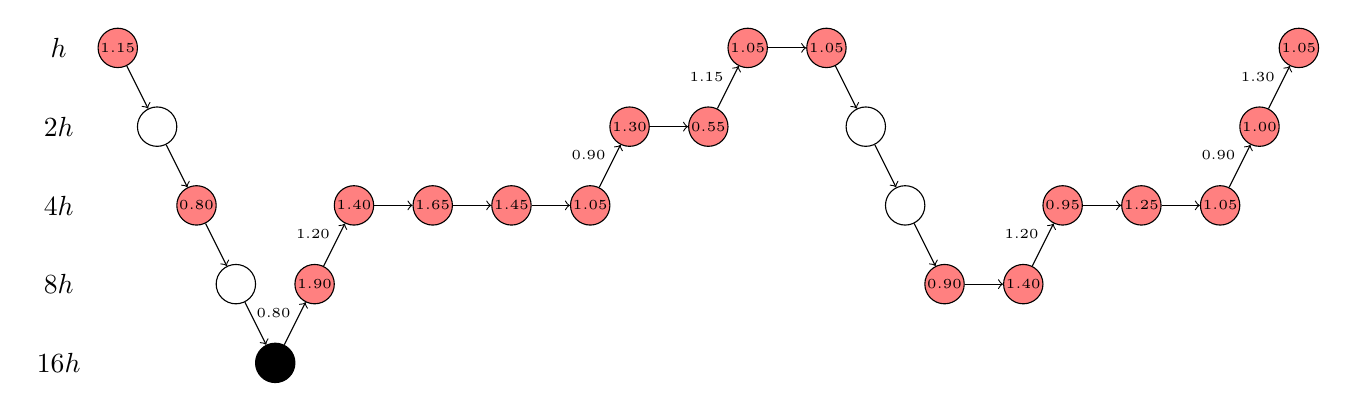
\begin{tikzpicture}
				\node   (h) at (-0.75, 4){$h$};
				\node   (2h) at (-0.75, 3){$2h$};
				\node   (4h) at (-0.75, 2){$4h$};
				\node   (8h) at (-0.75, 1){$8h$};
				\node   (16h) at (-0.75, 0){$16h$};
				\node	(a) at (0,4) [draw, fill=lightred, circle,inner sep=0pt,minimum size=5mm] {\tiny $1.15$};
				\node	(b) at (0.5,3) [draw, circle,inner sep=0pt,minimum size=5mm] {\phantom{\tiny $1.00$}};
				\node	(c) at (1,2) [draw, circle,fill=lightred,inner sep=0pt,minimum size=5mm] {\tiny $0.80$};
				\node	(d) at (1.5,1) [draw, circle,inner sep=0pt,minimum size=5mm] {\phantom{\tiny $1.00$}};
				\node	(e) at (2,0) [draw, circle,fill=black, inner sep=0pt,minimum size=5mm] {\phantom{\tiny $1.00$}};
				\node	(f) at (2.5,1) [draw, circle,  fill=lightred,inner sep=0pt,minimum size=5mm] {\tiny $1.90$};
				\node	(g) at (3,2) [draw, circle,fill=lightred,inner sep=0pt,minimum size=5mm] {\tiny $1.40$};
				\node	(h) at (4,2) [draw, circle,fill=lightred,inner sep=0pt,minimum size=5mm] {\tiny $1.65$};
				\node	(i) at (5,2) [draw, circle,fill=lightred,inner sep=0pt,minimum size=5mm] {\tiny $1.45$};
				\node	(j) at (6,2) [draw, circle,fill=lightred,inner sep=0pt,minimum size=5mm] {\tiny $1.05$};
				\node	(k) at (6.5,3) [draw, circle,fill=lightred,inner sep=0pt,minimum size=5mm] {\tiny $1.30$};
				\node	(l) at (7.5,3) [draw, circle,fill=lightred,inner sep=0pt,minimum size=5mm] {\tiny $0.55$};
				\node	(m) at (8,4) [draw, circle,fill=lightred,inner sep=0pt,minimum size=5mm] {\tiny $1.05$};
				\node	(n) at (9,4) [draw, circle,fill=lightred,inner sep=0pt,minimum size=5mm] {\tiny $1.05$};
				\node	(o) at (9.5,3) [draw, circle, inner sep=0pt,minimum size=5mm] {\phantom{\tiny $1.00$}};
				\node	(p) at (10,2) [draw, circle, inner sep=0pt,minimum size=5mm] {\phantom{\tiny $1.00$}};
				\node	(q) at (10.5,1) [draw, circle, fill=lightred, inner sep=0pt,minimum size=5mm] {\tiny $0.90$};
				\node	(r) at (11.5,1) [draw, circle, fill=lightred, inner sep=0pt,minimum size=5mm] {\tiny $1.40$};
				\node	(s) at (12,2) [draw, circle, fill=lightred, inner sep=0pt,minimum size=5mm] {\tiny $0.95$};
				\node	(t) at (13,2) [draw, circle, fill=lightred, inner sep=0pt,minimum size=5mm] {\tiny $1.25$};
				\node	(u) at (14,2) [draw, circle, fill=lightred, inner sep=0pt,minimum size=5mm] {\tiny $1.05$};
				\node	(v) at (14.5,3) [draw, circle, fill=lightred, inner sep=0pt,minimum size=5mm] {\tiny $1.00$};
				\node	(w) at (15,4) [draw, circle, fill=lightred, inner sep=0pt,minimum size=5mm] {\tiny $1.05$};
				\draw 
				(a) edge[->] (b) 
				(b) edge[->] (c)
				(c) edge[->] (d)
				(d) edge[->] (e)   
				(e) edge[->] node[near end,left] {\tiny 0.80} (f)
				(f) edge[->] node[near end,left] {\tiny 1.20} (g)
				(g) edge[->] (h)
				(h) edge[->] (i)
				(i) edge[->] (j) 
				(j) edge[->] node[near end,left] {\tiny 0.90} (k)
				(k) edge[->] (l)
				(l) edge[->] node[near end,left] {\tiny 1.15} (m)   
				(m) edge[->] (n)
				(n) edge[->] (o)
				(o) edge[->] (p)
				(p) edge[->] (q)
				(q) edge[->] (r)
				(r) edge[->] node[near end,left] {\tiny 1.20} (s)
				(s) edge[->] (t)
				(t) edge[->] (u)
				(u) edge[->] node[near end,left] {\tiny 0.90} (v)
				(v) edge[->] node[near end,left] {\tiny 1.30} (w)
				;
			\end{tikzpicture}
		}
	\caption{2D Poisson: ES-10}
	\label{fig:evolved-methods-graphical-representation:2D}
	\end{subfigure}
	\begin{subfigure}[t]{\columnwidth}
	\scalebox{0.75}{%
		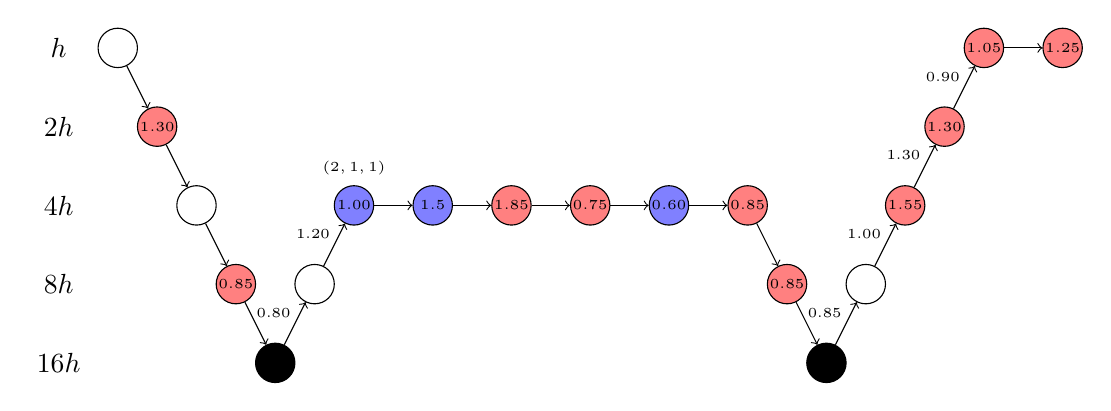
\begin{tikzpicture}
			\node   (h) at (-0.75, 4){$h$};
			\node   (2h) at (-0.75, 3){$2h$};
			\node   (4h) at (-0.75, 2){$4h$};
			\node   (8h) at (-0.75, 1){$8h$};
			\node   (16h) at (-0.75, 0){$16h$};
			\node	(a) at (0,4) [draw, circle,inner sep=0pt,minimum size=5mm] {\phantom{\tiny $1.00$}};
			\node	(b) at (0.5,3) [draw, circle, fill=lightred, inner sep=0pt,minimum size=5mm] {\tiny $1.30$};
			\node	(c) at (1,2) [draw, circle,inner sep=0pt,minimum size=5mm] {\phantom{\tiny $1.00$}};
			\node	(d) at (1.5,1) [draw, circle,fill=lightred, inner sep=0pt,minimum size=5mm] {\tiny $0.85$};
			\node	(e) at (2,0) [draw, circle,fill=black, inner sep=0pt,minimum size=5mm] {\phantom{\tiny $1.00$}};
			\node	(f) at (2.5,1) [draw, circle,inner sep=0pt,minimum size=5mm] {\phantom{\tiny $1.00$}};
			\node	(g) at (3,2) [draw, circle,fill=lightblue,inner sep=0pt,minimum size=5mm, label=above:{\tiny $(2,1,1)$}] {\tiny 1.00}; %TODO add block info
			\node	(h) at (4,2) [draw, circle,fill=lightblue,inner sep=0pt,minimum size=5mm] {\tiny $1.5$};
			\node	(i) at (5,2) [draw, circle,fill=lightred,inner sep=0pt,minimum size=5mm] {\tiny $1.85$};
			\node	(j) at (6,2) [draw, circle,fill=lightred,inner sep=0pt,minimum size=5mm] {\tiny $0.75$};
			\node	(k) at (7,2) [draw, circle,fill=lightblue,inner sep=0pt,minimum size=5mm] {\tiny $0.60$};
			\node	(l) at (8,2) [draw, circle,fill=lightred,inner sep=0pt,minimum size=5mm] {\tiny $0.85$};
			\node	(m) at (8.5,1) [draw, circle,fill=lightred,inner sep=0pt,minimum size=5mm] {\tiny $0.85$};
			\node	(n) at (9,0) [draw, circle,fill=black,inner sep=0pt,minimum size=5mm] {\phantom{\tiny $1.00$}};
			\node	(o) at (9.5,1) [draw, circle,inner sep=0pt,minimum size=5mm] {\phantom{\tiny $1.00$}};
			\node	(p) at (10,2) [draw, circle,  fill=lightred, inner sep=0pt,minimum size=5mm] {\tiny $1.55$};
			\node	(q) at (10.5,3) [draw, circle, fill=lightred, inner sep=0pt,minimum size=5mm] {\tiny $1.30$};
			\node	(r) at (11,4) [draw, circle, fill=lightred, inner sep=0pt,minimum size=5mm] {\tiny $1.05$};
			\node	(s) at (12,4) [draw, circle, fill=lightred, inner sep=0pt,minimum size=5mm] {\tiny $1.25$};
			\draw 
			(a) edge[->] (b) 
			(b) edge[->] (c)
			(c) edge[->] (d)
			(d) edge[->] (e)   
			(e) edge[->] node[near end,left] {\tiny 0.80} (f)
			(f) edge[->] node[near end,left] {\tiny 1.20} (g)
			(g) edge[->] (h)
			(h) edge[->] (i)
			(i) edge[->] (j) 
			(j) edge[->] (k)
			(k) edge[->] (l)
			(l) edge[->] (m)   
			(m) edge[->] (n)
			(n) edge[->] node[near end,left] {\tiny 0.85}(o)
			(o) edge[->] node[near end,left] {\tiny 1.00}(p)
			(p) edge[->] node[near end,left] {\tiny 1.30}(q)
			(q) edge[->] node[near end,left] {\tiny 0.90}(r)
			(r) edge[->] (s)
			;
		\end{tikzpicture}
	}
	\caption{3D Poisson: ES-9}
	\label{fig:evolved-methods-graphical-representation:3D}
	\end{subfigure}
	\caption{Computational structure of the evolved multigrid methods. The color of the node denotes the type of operation. Black: Coarse-grid solver, Blue: Block Jacobi smoothing, Red: Red-black Gauss-Seidel smoothing, White: No operation. The relaxation factor of each smoothing step is included in each node, while for coarse-grid correction, it is attached to the respective edge. For block smoothers, the dimension of the block is specified on top of the respective node. If no block size is specified, pointwise smoothing is applied.}
	\label{fig:evolved-methods-graphical-representation}
\end{figure}
The first observation that can be made from investigating the computational structure of these methods is that none of them can be clearly characterized as a V-, F- or W-cycle.
It is, therefore, impossible to formulate each of them within the framework of classical multigrid cycles, as shown in Algorithm~\ref{alg:multigrid-cycle}.
While, for instance, the first part of Figure~\ref{fig:evolved-methods-graphical-representation:2D} can be characterized as a V-cycle, the method then proceeds with an additional coarse-grid correction step that is based on a purely smoothing-based error reduction on the coarser levels.
Figure~\ref{fig:evolved-methods-graphical-representation:3D} starts off in a similar fashion but then applies an additional three-grid V-cycle on the third-finest level with a step size of $4h$, before it transfers the computed correction back to the finest level.
The analysis performed in the recent work by Avnat and Yavneh already suggests that employing cycles of non-classical structure can lead to a significantly higher degree of efficiency in solving certain PDEs~\cite{avnat2022recursive}. 
However, in addition to their non-classical structure, both multigrid methods employ a different number of smoothings steps on each level using a wide range of different relaxation factors, whereby, in general, on certain levels, significantly more smoothing is performed than on others.
In particular, smoothing on the third-finest level seems to be exceptionally effective in reducing the most significant error components, and hence, the number of smoothing steps on this level is higher than on any other level.
While both methods predominantly employ RB-GS as a smoother, Figure~\ref{fig:evolved-methods-graphical-representation:3D} also includes individual pointwise and block Jacobi steps.
Finally, the even more complicated computational structure of the methods discovered for the linear elastic boundary prevents us from including their graphical representations similar to Figure~\ref{fig:evolved-methods-graphical-representation}.
However, if we consider the evolved method ES-2, which leads to the fastest solving time for the larger instance of the linear elastic boundary value problem with $l_{max} = 11$, we can observe a number of structural similarities with the methods shown in Figure~\ref{fig:evolved-methods-graphical-representation}.
In particular, the method applies the coarse-grid solver only once within its computations and, therefore, resembles a V-cycle but also includes additional smoothing-based coarse-grid correction steps with a varying amount of smoothing on each level.
Furthermore, with the exception of a single Jacobi step on the second-coarsest level, the method employs exclusively RB-GS smoothing.

\section{Discovering Generalizable Multigrid-Based Preconditioners for the Helmholtz Equation}
While within the last section, we could already demonstrate that our evolutionary program synthesis approach leads to the automated design of multigrid methods with competitive performance compared to common multigrid cycles, none of the PDEs considered there is particularly challenging to solve.   
Therefore, in order to evaluate whether our approach can achieve any advantages compared to state-of-the-art methods in the case of a problem that is difficult to solve numerically, we consider the indefinite Helmholtz equation.
At this point, we would like to point out that all results presented in this section have been originally published in~\cite{schmitt2022evolving}.
The Helmholtz equation, whose basic form is given as 
\begin{equation}
	-\nabla ^{2}u - k^{2}u = f,
	\label{eq:helmholtz}
\end{equation} 
is a famously-difficult test problem for the application of numerical methods that also has practical relevance for many real-world applications, such as~\cite{versteeg1994marmousi,martin2006marmousi2,billette20052004,gray1995migration}.
The main difficulty in solving this equation is that the system of linear equations resulting from its discretization becomes highly ill-conditioned for large values of the wavenumber $k$~\cite{ernst2012difficult}.
If we, for instance, assume the use of ten grid points per wavelength\footnote{Usually the relation of the wavelength $\lambda$ to the wavenumber $k$ is defined as $k = 2 \pi/\lambda$ }, as it is common in geophysical applications~\cite{erlangga2006multigrid}, on the dimensionless unit square, a second-order accuracy requirement of $kh = 0.625$ must be fulfilled.
Figure~\ref{fig:condition-number-helmholtz} shows the condition number of the system matrix $A$ that results from a discretization of Equation~\eqref{eq:helmholtz} for different values of the wavenumber $k$.
\begin{figure}
		\centering
		\includegraphics[width=\textwidth]{figures/cond.pdf}
		\caption{Condition number of the system matrix resulting from a finite-difference discretization of the two-dimensional Helmholtz equation with $kh = 0.625$}
		\label{fig:condition-number-helmholtz}
\end{figure}
The condition number gives us a measure of how much an initial approximation error is magnified by the application of the operator $A$.
As we can see in Figure~\ref{fig:condition-number-helmholtz} for larger values of $k$, the condition number of $A$ increases dramatically, which leads to an extreme accumulation of numerical errors. 
The necessity to handle these errors makes the design of an efficient or even functioning numerical method for the indefinite Helmholtz equation outstandingly difficult.
In particular, without any modification, classical multigrid methods can not effectively be applied as a numerical solver for indefinite Helmholtz problems~\cite{ernst2012difficult}.
One multigrid-based approach that mitigates this problem is the application of the method as a preconditioner instead of applying it to the discretized Helmholtz system directly.
In general, preconditioning has the purpose of modifying a given system of linear equations by applying a so-called preconditioning matrix $M$ in order to obtain a new system that is then easier to solve.
For instance, right-preconditioning the system $A \bm{x} = \bm{b}$ with the matrix $M$ results in
\begin{equation}
	A M^{-1} \bm{y} = \bm{b},
	\label{eq:right-preconditioning}
\end{equation}
with $M \bm{x} = \bm{y}$. 
The main consequence of this formulation is that we now have to solve an additional system of linear equations in the form of $M \bm{x} = \bm{y}$ whenever the operator $A$ is applied within our original solution method.
If we consider the extreme choice of $M$ as the original operator $A$, this means that Equation~\eqref{eq:right-preconditioning} reduces to $I \bm{y} = \bm{b}$, however, with the consequence that the system $M \bm{x} = \bm{y}$ becomes just as ill-conditioned as the original one.
Therefore, the choice of the preconditioning matrix $M$ usually represents a compromise between the accurate approximation of the original matrix $A$ and the ease of solvability of $M \bm{x} = \bm{y}$~\cite{benzi2002preconditioning}.
Since its invention by Erlangga et al.~\cite{erlangga2004preconditioner}, the choice of $M$ as a complex-shifted version of the original operator has proven its effectiveness for indefinite Helmholtz problems~\cite{erlangga2008advances,cocquet2017shift,umetami2009multigrid,cools2013analysis}, which leads to
\begin{equation*}
	M = -\nabla ^{2} - (k^{2} + i \varepsilon).
\end{equation*}
%TODO include all suitable citations
As it has been shown in~\cite{cocquet2017shift}, a shift $\varepsilon \approx \mathcal{O}(k^2)$ enables the efficient inversion of $M$ by multigrid, whereas the choice of a smaller shift increases the preconditioning effectiveness.
Since the resulting linear system, $A M^{-1} \bm{y} = \bm{b}$ is often complex-symmetric but non-hermitian, it is commonly solved using a suitable Krylov subspace method, such as GMRES and BiCGSTAB~\cite{saad2003iterative}.
\subsection{Problem Formulation}
After introducing the indefinite Helmholtz equation and the difficulties its solution comprises in a general manner, we can now proceed by defining a representative instance of this equation for the evaluation of our grammar-based approach for the automated design of multigrid methods.
For this purpose, we consider the two-dimensional Helmholtz equation on a unit square with Dirichlet boundary conditions at the top and bottom and Robin radiation conditions at the left and right, as given by
\begin{equation}
	\label{eq:helmholtz-test-problem}
	\begin{split}
		(-\nabla ^{2} - k^{2}) u & = f \quad \text{in} \; \left( 0, 1 \right)^2 \\
		u & = 0 \quad \text{on} \; \left( 0, 1 \right) \times \{0\}, \left( 0, 1 \right) \times \{1\} \\
		\partial_{\mathbf{n}} u - iku & = 0 \quad \text{on} \; \{0\} \times \left( 0, 1 \right), \{1\} \times \left( 0, 1 \right) \\
		f(x, y) & = \delta(x - 0.5, y - 0.5),
	\end{split}
\end{equation}
where $\delta(\bm{x})$ is the Dirac delta function.
We discretize this equation on a uniform Cartesian grid using the classical five-point stencil
\begin{equation*}
	A_h = \frac{1}{h^2} \begin{bmatrix}
		& -1 & \\
		-1 & 4 - (k h)^2 & -1 \\
		& -1 &  
	\end{bmatrix}.
\end{equation*}
In addition, $\delta(\bm{x})$ is approximated with a second-order Zenger correction~\cite{koestler2004extrapolation}.
The spacing $h$ of the grid is chosen to fulfill the second-order accuracy requirement $h k = 0.625$ as described above.
Finally, we apply the shifted-Laplace
\begin{equation*}
	M = -\nabla^{2} - (k^{2} + 0.5 i k^{2}),
\end{equation*}
suggested in~\cite{erlangga2008advances} as a preconditioner, which is discretized similarly to the original operator using the five-point stencil
\begin{equation*}
	M_h = \frac{1}{h^2} \begin{bmatrix}
		& -1 & \\
		-1 & 4 - (1.0 + 0.5i)(k h)^2 & -1 \\
		& -1 &  
	\end{bmatrix}.
\end{equation*}
\subsection{Solver Configuration}
\label{sec:solver-configuration-helmholtz}
As a result of the above formulation of our test problem, we obtain two systems of linear equations
\begin{equation}
	A_h M_h^{-1} \bm{y}_h = \bm{b}_h,
	\label{eq:helmholtz-test-problem-discretized-and-preconditioned}
\end{equation}
where $\bm{b}_h$ contains the values of $\delta(\bm{x})$ at each grid point, and
\begin{equation}
	M_h \bm{x}_h = \bm{y}_h,
	\label{eq:helmholtz-test-problem-preconditioning}
\end{equation}
where $\bm{x}_h$ represents the approximate solution of Equation~\eqref{eq:helmholtz-test-problem}.
While for each of these two systems of linear equations, a functioning solver is needed, the focus of our experimental evaluation is the design of an efficient multigrid method for the approximate solution of Equation~\eqref{eq:helmholtz-test-problem-preconditioning}.
Here, to limit the cost of preconditioning, as in~\cite{erlangga2008advances}, we assume that the application of a single multigrid cycle is sufficient to compute a reasonable approximation for $M_{h}^{-1}$.
After designing a suitable multigrid-based preconditioner, Equation~\eqref{eq:helmholtz-test-problem-discretized-and-preconditioned} is then solved using the biconjugate gradient stabilized method (BiCGSTAB)~\cite{saad2003iterative}.
The resulting iterative solution scheme is summarized in Algorithm~\ref{alg:preconditioned-bicgstab}, in which, for the sake of simplicity, we omit the grid spacing $h$.
\begin{algorithm}[t]
	\caption{Right-Preconditioned BiCGSTAB}
	\label{alg:preconditioned-bicgstab}
	\begin{algorithmic}[1] % The number tells where the line numbering should start
			\State $\bm{r}^0 = \bm{b} - A \bm{x}^0$
			\State $\bm{\hat{r}}^0 = \bm{r}^0$
			\State $\alpha_0 = \beta_0 = \rho_0 = \omega_0 = 1$
			\State $\bm{p}^0 = \bm{q}^0 = \bm{0}$
			\For{$i := 1, \dots, n$}
			\State $\rho_i = \bm{\hat{r}}^{i-1} \cdot \bm{r}^{i-1}$
			\State $\beta_i = \frac{\rho_i }{\rho_{i-1} }\frac{\alpha_{i-1}}{ \omega_{i-1}}$
			\State $\bm{p}^i = \bm{r}^{i-1} + \beta_i (\bm{p}^{i-1} - \omega_{i-1} \bm{q}^{i-1})$
			\State Solve $M \bm{x}^i = \bm{p}^i$
			\State $\bm{q}^i = A \bm{x}^i$
			\State $\alpha_i = \rho_i / (\bm{\hat{r}}^{i-1} \cdot \bm{q}^i)$
			\State $\bm{h}^i = \bm{x}^{i-1} + \alpha_i \bm{x}^i$	
			\State $\bm{s}^i = \bm{r}^{i-1} - \alpha_i \bm{r}^i$
			\State Solve $M \bm{x}^i = \bm{s}^i$
			\State $\bm{t}^i = A \bm{x}^i$
			\State $\omega_i = (\bm{t}^i \cdot \bm{s}^i) / (\bm{t}^i \cdot \bm{t}^i)$
			\State $\bm{x}^i = \bm{h}^i + \omega_i \bm{x}^i$
			\State $\bm{r}^i = \bm{s}^i - \omega_i \bm{t}^i$
			\If{$\norm{\bm{r}^i}/\norm{\bm{r}^0} < \epsilon$}
			\Return $\bm{x}^i$
			\EndIf
			\EndFor
		\end{algorithmic}
\end{algorithm}
In each step of this iterative scheme, it is necessary to compute an approximate solution for two systems of linear equations in the form of $M \bm{x}^i = \bm{y}^i$, %, in line 9 and 14, 
which is achieved in both cases by applying a single multigrid cycle.
To construct an efficient method for this purpose, we consider the set of five-grid methods that are defined on a hierarchy of discretization with $h = 1/2^{l}$ on each level $l \in \left[l_{max} - 4,l_{max}\right]$. 
Similar to Section~\ref{sec:experiments-part1}, we then consider the following components within each step of the method:
\begin{description}
	\item[\textbf{Smoothers}:] Pointwise and block Jacobi with rectangular blocks up to a maximum number of six terms, red-black Gauss-Seidel (RB-GS)
	\item[\textbf{Restriction}:] Full-weighting restriction
	\item[\textbf{Prolongation}:] Bilinear interpolation
	\item[\textbf{Relaxation factors}:] $\left( 0.1 + 0.05i \right)_{i = 0}^{36} = \left(0.1, 0.15, 0.2, \dots, 1.9 \right)$
	\item[\textbf{Coarse-grid solver}:] BiCGSTAB for $l = l_{max} - 4$
\end{description}
The resulting multigrid grammar is similar to the one shown in Table~\ref{table:multigrid-grammar}, however, with the modification that each occurrence of a system matrix $A_H$ and right-hand side $\ps{b_H}$ is replaced by the respective preconditioning matrix $M_H$ and right-hand side $\ps{y_H}$.
Similar to Section~\ref{sec:experiments1-multigrid-configuration}, block Jacobi smoothers are generated based on rectangular blocks of grid points, while the relaxation factor $\omega$ of each smoothing and coarse-grid correction step is chosen from the above interval.
To assess the efficiency and generalizability of the multigrid preconditioners evolved with our approach, we consider the set of possible multigrid cycles that can be constructed based on the classical formulation of these methods, using the same components as described above.
To ensure that each method uses the optimal smoother and relaxation factor, we evaluate each possible combination from the available set of options on the largest problem size for which convergence can be achieved.
Due to the ill-conditioning of the indefinite Helmholtz equation, we consider an approximate solution to be sufficient when the initial residual has been reduced by a factor of $10^{-7}$ for $k \leq 160$ and $10^{-6}$ for all larger wavenumbers.

\subsection{Experimental Settings and Evaluation Platform}
In Section~\ref{sec:experiments-part1}, due to the relative simplicity of the problems considered, along with the fact that our main focus has been to gain an understanding of the general behavior of our evolutionary algorithm, we kept the problem size constant throughout each experiment.
However, in the case of the indefinite Helmholtz equation, this strategy is infeasible due to a number of reasons.
First of all, doubling the wavenumber requires us to use twice as many grid points in each dimension because of the requirement $kh = 0.625$, which means that we end up with a system of linear equations that is not only significantly worse conditioned but also has four times the number of unknowns.
As a consequence, solving Helmholtz problems with a large wavenumber becomes tremendously expensive, which makes the evaluation of a large number of different preconditioners infeasible.
Furthermore, in practice, our goal is to design multigrid methods that can be applied to a wide range of different problem instances, and thus, generalizability is one of our main concerns.
In Section~\ref{sec:generalization-procedure}, we have already proposed a systematic procedure for the generalization of a population of individuals to multiple instances of the same problem.
This method aims to evolve a population of generalizable multigrid methods by iteratively increasing the size of the test problem considered within the evaluation of each solver after a certain number of generations $m$.
While the formulation of our problem based on the wavenumber-dependent grid spacing $h$ allows us to construct problem instances of larger size and difficulty in a straightforward manner, it is unclear after how many generations this operation should be performed.
However, in the experiments performed in Section~\ref{sec:experiments-part1}, we could observe that the majority of improvement in both objectives is achieved within the first 50 generations of our evolutionary algorithm.
Therefore, setting the generalization interval $m$ to 50 represents a reasonable compromise between allowing the population to adapt to modified conditions and preventing it from overfitting to the characteristics of a particular problem instance.
To initiate the execution of our evolutionary algorithm, we choose $k = 80$ as a problem instance, which leads to a maximum level $l_{max} = 7$ and a system of linear equations consisting of 16129 unknowns. 
Therefore, the cost of evaluation at the beginning is significantly lower compared to later generations.
We then execute Algorithm~\ref{alg:generalization-procedure} with a population size of 128 and a total number of 150 generations, whereby after 50 and 100 generations, we increase the value of wavenumber to 160 and 320, respectively.
Table~\ref{table:gp-parameters-helmholtz} gives an overview of the algorithmic parameters used for each experiment, which are mostly similar to the ones employed in Section~\ref{sec:experiments-part1}.
\begin{table}
	\centering
	\caption{Summary of GGGP configuration parameters.}
	\label{table:gp-parameters-helmholtz}
	\begin{tabular}{l c}
		\toprule
		Parameter & Value \\
		\midrule 
		Evolutionary algorithm type & $(\mu + \lambda)$ \\
		\midrule
		Objectives & $t, n$ \\
		\midrule
		Number of generations & 150 \\
		\midrule
		$k$ & 80, 160, 320 \\
		\midrule
		Generalization interval & 50 \\
		\midrule
		Initial population size & 1024 \\
		\midrule
		$\lambda$ & 128 \\
		\midrule
		$\mu$ & 128 \\
		\midrule
		Number of MPI processes & 64 \\
		\midrule
		Non-dominated sorting procedure & \cite{deb2002fast} \\ 
		\midrule
		Selection operator & \cite{deb2002fast} \\ 
		\midrule
		Crossover operator & Single-point crossover \\
		\midrule
		Crossover probability & $2/3$ \\
		\midrule
		Mutation operator & Random subtree insertion \\
		\midrule 
		Probability to mutate a terminal symbol & $1/3$ \\
		\bottomrule
	\end{tabular}
\end{table}
In order to evaluate each multigrid method, we measure the number of iterations $n$ Algorithm~\ref{alg:preconditioned-bicgstab} requires to achieve the desired defect reduction for Equation~\ref{eq:helmholtz-test-problem-discretized-and-preconditioned} together with its execution time per iteration $t$.
These two metrics then serve as the two objectives for our multi-objective evolutionary algorithm.
Note that in previous formulations of our method, we have employed the solver's convergence factor $\rho$ as a first objective.
However, due to the difficulty of the problem considered here, we expect the average number of iterations to achieve the desired defect reduction to be significantly larger than in our previous experiments. 
Therefore, the potentially small difference relative to the total number of iterations between two preconditioners means that the absolute values of their convergence factors are hardly distinguishable~\footnote{Note that the convergence factor is estimated by computing the n-th root of the product of the measured defect reductions in each iteration, as given by Equation~\eqref{eq:asymptotic_convergence_factor}}, which has the potential to lead to the accumulation of numerical errors in the computation of population-density metrics, such as the crowding distance~\cite{deb2002fast}.
Using the number of iterations instead as the first objective avoids this issue, while, due to the ill-conditioning of the considered problem, even a small improvement in the accuracy of the preconditioner will lead to a measurable decrease in the value of this metric.

Similar to Section~\ref{sec:experiments-part1}, we select individuals for crossover and mutation using a binary tournament selection based on their dominance relation and crowding distance.
New individuals are again created using a single-point crossover with a probability of 2/3 and random subtree insertion with a probability of 1/3, whereby in the latter case, we insert the generated subtree whenever possible within the selected branch and otherwise replace it completely, as described in Section~\ref{sec:gggp-mutation-and-recombination}.

To evaluate the effectiveness of our evolutionary program synthesis approach, we perform a total number of ten experiments with a random initialization, each of which is executed on SuperMUC-NG\footnote{SuperMUC-NG: \url{https://doku.lrz.de/display/PUBLIC/SuperMUC-NG}}.
Even though the population size, as well as the number of generations, is smaller than within our experimental evaluation in Section~\ref{sec:experiments-part1}, the time required to evaluate each solver drastically increases for larger wavenumbers, leading to an overall higher computational cost of each optimization run.
To parallelize our evolutionary search method, we employ an MPI-based described in Section~\ref{sec:distributed-parallelization} using 64 MPI processes that are distributed to eight compute nodes of the system, where each process is exclusively executed on one of the eight available islands.
Therefore, each process creates and evaluates two new individuals per generation, which are then executed on the respective island using on OpenMP-based shared-memory parallelization with 12 threads.

\subsection{Reference Methods}
To assess whether our evolutionary program synthesis method can discover competitive multigrid preconditioners for the indefinite Helmholtz equation, we first need to investigate the preconditioning efficiency of classical multigrid cycles.
As in previous evaluations, we consider the time required to achieve a certain error reduction as a measure of the efficiency of a solver.
However, since in the given case, we apply the same iterative solver to each problem instance but vary the multigrid cycle used for preconditioning, this metric instead relates to the efficiency of the latter.
For instance, a multigrid cycle that is able to compute an improved approximation of the solution of the preconditioning system, as given by Equation~\eqref{eq:helmholtz-test-problem-preconditioning}, reduces the number of iterations required for solving the preconditioned system, which, however, might come at the prize of a higher computational cost.
The second quality metric that we aim to investigate in this section is the capability of each multigrid preconditioner to generalize to different instances of the same problem.
Therefore, we consider three different wavenumbers $k = 160, 320$, and $640$ for the evaluation of each method, which we perform on a single compute node of SuperMUC-NG using an OpenMP-based shared-memory parallelization  with 48 threads, such that each thread is executed on a dedicated CPU core.
As a multigrid-based preconditioner, we then consider different V, W, and F-cycles with up to five pre and post-smoothing steps based on the configuration space described in Section~\ref{sec:solver-configuration-helmholtz}.
As in previous works on multigrid-based preconditioners for the indefinite Helmholtz equation~\cite{erlangga2006multigrid,erlangga2008advances,cocquet2017shift}, the same smoother and relaxation factor is applied for a fixed number of steps on each level.
To find out which combination of smoother and relaxation factor works best for each cycle, we have first tested each of them on the largest and, hence, worst conditioned problem with $k = 640$.
However, since none of the available configuration options led to a converging solver for this case, we instead employ the next smaller problem size with a wavenumber of $k = 320$ to find out which pair of smoother and relaxation factor leads to the fastest solving time for each multigrid cycle.
In general, according to our experimental evaluation RB-GS represents the single most efficient smoother for the given case, while Jacobi-type smoothers only lead to a converging solver for wavenumbers of at most $k = 160$, with, however, less efficiency in all cases than the former.
Therefore, Table~\ref{table:reference-methods-helmholtz} shows the resulting average solving times for each multigrid cycle with RB-GS smoothing and an optimum relaxation factor for $k = 320$, where the omission of a number means that convergence could not be achieved within 20,000 iterations. 
Since the use of more than three pre and post-smoothing steps did not yield any additional benefit, we have omitted all multigrid cycles with a higher number of smoothing steps.
\begin{table}
	\caption{Reference methods - Optimum relaxation factors $\omega$ for $k = 320$, number of iterations, and the average time required for solving a problem with the particular wavenumber.}
	\label{table:reference-methods-helmholtz}
	\centering
	\begin{tabular}{l l l l l l}
		\toprule
		& $\omega$ & \multicolumn{2}{c}{Iterations} & \multicolumn{2}{c}{Solving Time (s)} \\
		\cmidrule(r){3-4} \cmidrule(r){5-6}
		$k$ & & $160$ & $320$ & $160$ & $320$ \\
		\midrule
		V(0, 1) & $1.25$ & $2078$ & $6297$ & $6.38$ & $35.11$ \\
		\midrule
		V(1, 1) & $0.6$ & $1880$ & $6297$ & $7.66$ & $44.27$ \\
		\midrule
		V(2, 1) & $0.6$ & $-$ & $5532$ & $-$ & $47.0$ \\
		\midrule
		V(2, 2) & $0.5$ & $1627$ & $5115$ & $9.93$ & $50.54$  \\
		\midrule
		V(3, 3) & $0.4$ & $1753$ & $5168$ & $13.97$ & $76.00$ \\
		\midrule
		F(0, 1) & $1.15$ & $1467$ & $4028$ & $8.15$ & $42.87$  \\
		\midrule
		F(1, 1) & $0.75$ & $1546$ & $3988$ & $11.21$ & $54.51$ \\
		\midrule
		F(2, 1) & $0.55$ & $1146$ & $3934$ & $10.87$ & $67.62$ \\
		\midrule
		F(2, 2) & $0.65$ & $1060$ & $3213$ & $13.92$ & $65.06$ \\
		\midrule
		F(3, 3) & $0.45$ & $1085$ & $3464$ & $18.88$ & $92.97$ \\
		\midrule
		W(0, 1) & $0.75$ & $1265$ & $4215$ & $8.67$ & $72.08$ \\
		\midrule
		W(1, 1) & $0.8$ & $1208$ & $3570$ & $13.08$ & $76.22$ \\
		\midrule
		W(2, 1) & $0.6$ & $1313$ & $3074$ & $17.71$ & $79.67$ \\
		\midrule
		W(2, 2) & $0.5$ & $1069$ & $3376$ & $17.14$ & $101.6$ \\
		\midrule
		W(3, 3) & $0.45$ & $942$ & $2976$ & $19.65$ & $117.8$ \\
		\bottomrule
	\end{tabular}
\end{table}
To eliminate the variability between individual measurements, each value contained in the table represents the average of 50 solver executions.
As expected, a higher number of smoothing steps and coarse-grid corrections increases the efficiency of the preconditioner and, thus, leads to a lower number of iterations until convergence.
However, if we consider the configuration that leads to the fastest solving time, which is the V(0,1), we can see that a single coarse-grid correction followed by a single step of RB-GS smoothing is actually the best choice for all wavenumbers considered.
After determining the best possible configuration for each classical multigrid cycle, we can finally investigate whether the multigrid methods designed with our evolutionary program synthesis method are able to achieve the same degree of efficiency and generalizability in preconditioning indefinite Helmholtz problems.
\subsection{Evaluation of the Evolved Multigrid Methods}
First, in order to identify the most promising multigrid-based preconditioners for our final evaluation, we sort the population at the end of each experiment according to the product of both objectives.
Note that while this metric corresponds to the solving time achieved on a single island, we intend to execute each method on a full node of the system, which can lead to a different outcome.
We then evaluate the ten best multigrid methods by employing them as a preconditioner for Equation~\eqref{eq:helmholtz-test-problem-preconditioning} with $k = 640$ while we measure the solving time of the resulting preconditioned iterative method.
In case none of the methods considered is able to reduce the initial residual by a factor of $10^{-6}$ within 20,000 iterations, we repeat the evaluation with the next smaller wavenumber $k = 320$.
The best-performing method is then evaluated on the full set of wavenumbers, i.e., $k = 160, 320, 640$.
Table~\ref{table:evolved-solvers} shows the required number of iterations and time to achieve the desired residual reduction when using each multigrid method as a preconditioner for Algorithm~\ref{alg:preconditioned-bicgstab}.
\begin{table}
	\caption{Best preconditioners according to the product of both objectives - Number of iterations and the average time required for solving a problem with the particular wavenumber.}
	\label{table:evolved-solvers}
	\centering
	\begin{tabular}{l l l l l l l }
		\toprule
		& \multicolumn{3}{c}{Iterations} & \multicolumn{3}{c}{Solving Time (s)} \\
		\cmidrule(l){2-4} \cmidrule(l){5-7}
		$k$ & $160$ & $320$ & $640$ & $160$ & $320$ & $640$ \\
		\midrule
		EP-1 & $1178$ & $3399$ & $-$ & $6.29$ & $28.07$ & $-$ \\
		\midrule
		EP-2 & $795$ & $2160$ & $8449$ & $7.86$ & $29.89$ & $241.7$\\
		\midrule
		EP-3 & $933$ & $2827$ & $11143$ & $6.08$ & $27.58$ & $257.8$ \\
		\midrule
		EP-4 & $637$ & $2509$ & $7901$ & $7.17$& $41.04$ & $268.2$ \\
		\midrule
		EP-5 & $539$ & $1838$ & $7765$ & $5.01$ & $28.39$ & $227.7$ \\
		\midrule
		EP-6 & $941$ & $2103$ & $-$ & $9.58$ & $30.76$ & $-$ \\
		\midrule
		EP-7 & $955$ & $2701$ & $-$  & $6.45$& $27.84$ & $-$ \\
		\midrule
		EP-8 & $945$ & $2870$ & $10839$ & $7.24$ & $33.02$ & $276.9$ \\
		\midrule
		EP-9 & $3436$ & $3872$ & $-$  & $15.15$ & $27.51$ & $-$ \\
		\midrule
		EP-10 & $586$ & $1881$ & $8855$ & $6.70$ & $31.39$ & $246.1$ \\
		\bottomrule
	\end{tabular}
\end{table}
With the exception of EP-4, the multigrid-based preconditioners discovered with our evolutionary program synthesis method all achieve faster solving times than the best reference method V(0,1) for $k = 320$, while, in the majority of cases, the same methods also work efficiently for $k = 160$.
If we consider the required number of iterations as a second metric, we can see that the methods discovered with our approach achieve at least a similar degree of preconditioning effectiveness as most W-cycles, however, with a significantly higher degree of computational efficiency.
Furthermore, even though the largest wavenumber considered within our evolutionary algorithm is $320$, in six out of ten experiments, our approach yields multigrid-based preconditioners that lead to a converging solver for $k = 640$, while all available reference methods fail to achieve convergence in this case.
Figure~\ref{fig:helmholtz-solving-time-comparison} shows a direct comparison of the preconditioners from both categories that lead to the fastest solving time for large wavenumbers.
\begin{figure}
	\includegraphics[width=\textwidth]{figures/solving-time.pdf}
	\caption{Solving time comparison of the best preconditioners according to the product of both objectives for different wavenumbers ($k$).}
	\label{fig:helmholtz-solving-time-comparison}
\end{figure} 
For better interpretability of the results, we have normalized each solving time by the number of grid points.
As the system of linear equations resulting from a discretization of Equation~\ref{eq:helmholtz-test-problem} becomes increasingly ill-conditioned for larger values of the wavenumber $k$, the relative cost to solve for each unknown grows accordingly.
All three discovered multigrid methods included in Figure~\ref{fig:helmholtz-solving-time-comparison} achieve a faster solving time than the best reference method V(0,1) while also staying competitive for smaller wavenumbers.
In particular, the overall best preconditioner EP-5 leads to a consistent improvement of 20 \% to the V(0,1) cycle.
\subsection{Algorithmic Analysis}
\begin{table}
	\caption{Operations per level}
	\label{table:operations-per-level}
	\centering
	\begin{tabular}{l c c c c c c c}
		\toprule
  		& \multicolumn{3}{c}{Smoothing} & \multicolumn{3}{c}{Coarse-Grid Correction} & \\
		\cmidrule(l){2-4} \cmidrule(l){5-7}
		Level & Mean & Min & Max & Mean & Min & Max & Total Mean \\
        \midrule
        $h$ & $1.17$ & $1$ & $2$ & $2.17$ & $1$ & $5$ & $3.33$\\
        \midrule
        $2h$ & $3.33$ & $2$ & $5$ & $4.50$ & $3$ & $6$ & $7.83$ \\
        \midrule
        $4h$ & $5.50$ & $3$ & $9$ & $1.83$ & $1$ & $4$ & $7.33$ \\
        \midrule
        $8h$ & $1.33$ & $0$ & $3$ & $1.17$ & $1$ & $2$ & $2.50$ \\
		\bottomrule
	\end{tabular}
\end{table}
To understand how the methods obtained with our approach represent more effective preconditioners than all known multigrid cycles, we can analyze their algorithmic structure.
For this purpose, Figure~\ref{fig:structure-evolved-preconditioners} contains a graphical representation of the two multigrid-based preconditioners, EP-5 and EP-2, that achieve the fastest solving times for $k = 640$.
\begin{figure}
	\begin{subfigure}[t]{\columnwidth}
		\scalebox{0.85}{%
			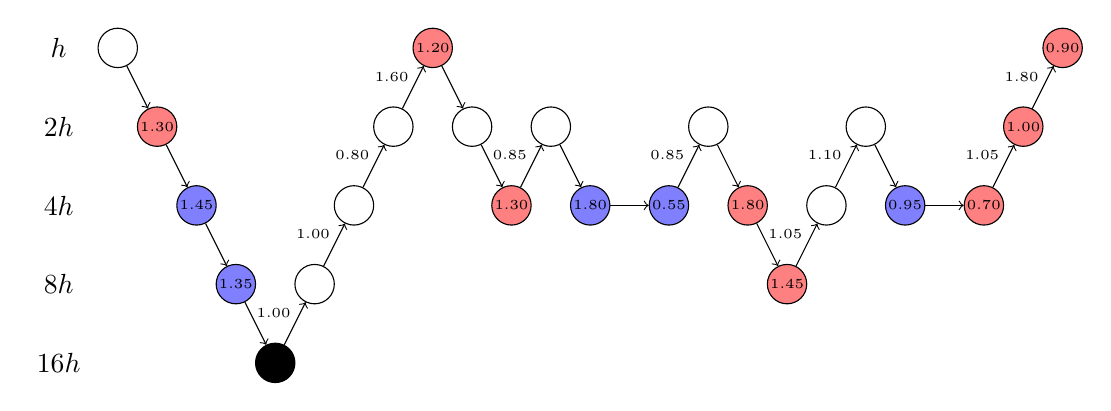
\begin{tikzpicture}
			\node   (h) at (-0.75, 4){$h$};
			\node   (2h) at (-0.75, 3){$2h$};
			\node   (4h) at (-0.75, 2){$4h$};
			\node   (8h) at (-0.75, 1){$8h$};
			\node   (16h) at (-0.75, 0){$16h$};
			\node	(a) at (0,4) [draw, circle,inner sep=0pt,minimum size=5mm] {\phantom{\tiny 1.00}};
			\node	(b) at (0.5,3) [draw, circle,fill=lightred,inner sep=0pt,minimum size=5mm] {\tiny 1.30};
			\node	(c) at (1,2) [draw,circle,fill=lightblue, inner sep=0pt,minimum size=5mm] {\tiny 1.45};
			\node	(d) at (1.5,1) [draw,circle,fill=lightblue, inner sep=0pt,minimum size=5mm] {\tiny 1.35};
			\node	(e) at (2,0) [draw, circle,fill=black, inner sep=0pt,minimum size=5mm] {\phantom{\tiny 1.00}};
			\node	(f) at (2.5,1) [draw, circle, inner sep=0pt,minimum size=5mm] {\phantom{\tiny 1.00}};
			\node	(g) at (3,2) [draw, circle, inner sep=0pt,minimum size=5mm] {\phantom{\tiny 1.00}};
			\node	(h) at (3.5,3) [draw, circle, inner sep=0pt,minimum size=5mm] {\phantom{\tiny 1.00}};
			\node	(i) at (4,4) [draw, circle,fill=lightred, inner sep=0pt,minimum size=5mm] {\tiny 1.20};
			\node	(j) at (4.5,3) [draw, circle, inner sep=0pt,minimum size=5mm] {\phantom{\tiny 1.00}};
			\node	(k) at (5,2) [draw, circle,fill=lightred, inner sep=0pt,minimum size=5mm] {\tiny 1.30};
			\node	(l) at (5.5,3) [draw, circle, inner sep=0pt,minimum size=5mm] {\phantom{\tiny 1.00}};
			\node	(m) at (6,2) [draw, circle,fill=lightblue, inner sep=0pt,minimum size=5mm] {\tiny 1.80};
			\node	(n) at (7,2) [draw, circle,fill=lightblue, inner sep=0pt,minimum size=5mm] {\tiny 0.55};
			\node	(o) at (7.5,3) [draw, circle, inner sep=0pt,minimum size=5mm] {\phantom{\tiny 1.00}};
			\node	(p) at (8,2) [draw, circle, fill=lightred, inner sep=0pt,minimum size=5mm] {\tiny 1.80};
			\node	(q) at (8.5,1) [draw, circle, fill=lightred, inner sep=0pt,minimum size=5mm] {\tiny 1.45};
			\node	(r) at (9,2) [draw, circle, inner sep=0pt,minimum size=5mm] {\phantom{\tiny 1.00}};
			\node	(s) at (9.5,3) [draw, circle, inner sep=0pt,minimum size=5mm] {\phantom{\tiny 1.00}};
			\node	(t) at (10,2) [draw, circle, fill=lightblue, inner sep=0pt,minimum size=5mm] {\tiny 0.95};
			\node	(u) at (11,2) [draw, circle, fill=lightred, inner sep=0pt,minimum size=5mm] {\tiny 0.70};
			\node	(v) at (11.5,3) [draw, circle, fill=lightred, inner sep=0pt,minimum size=5mm] {\tiny 1.00};
			\node	(w) at (12,4) [draw, circle, fill=lightred, inner sep=0pt,minimum size=5mm] {\tiny 0.90};
			\draw 
			(a) edge[->] (b) 
			(b) edge[->] (c)
			(c) edge[->] (d)
			(d) edge[->] (e)   
			(e) edge[->] node[near end,left] {\tiny 1.00}  (f)
			(f) edge[->] node[near end,left] {\tiny 1.00} (g)
			(g) edge[->] node[near end,left] {\tiny 0.80} (h)
			(h) edge[->] node[near end,left] {\tiny 1.60} (i)
			(i) edge[->] (j) 
			(j) edge[->] (k)
			(k) edge[->] node[near end,left] {\tiny 0.85} (l)
			(l) edge[->] (m)   
			(m) edge[->] (n)
			(n) edge[->] node[near end,left] {\tiny 0.85} (o)
			(o) edge[->] (p)
			(p) edge[->] (q)
			(q) edge[->] node[near end,left] {\tiny 1.05} (r)
			(r) edge[->] node[near end,left] {\tiny 1.10} (s)
			(s) edge[->] (t)
			(t) edge[->] (u)
			(u) edge[->] node[near end,left] {\tiny 1.05} (v)
			(v) edge[->] node[near end,left] {\tiny 1.80} (w)
			;
			\end{tikzpicture}
		}
		\caption{EP-5}
		\label{fig:ep-5}
	\end{subfigure}
	\begin{subfigure}[t]{\columnwidth}
		\scalebox{0.85}{%
			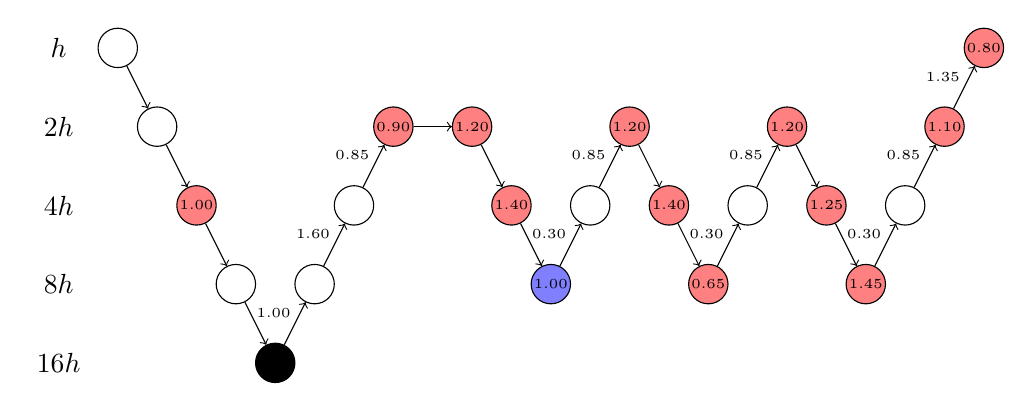
\begin{tikzpicture}
			\node   (h) at (-0.75, 4){$h$};
			\node   (2h) at (-0.75, 3){$2h$};
			\node   (4h) at (-0.75, 2){$4h$};
			\node   (8h) at (-0.75, 1){$8h$};
			\node   (16h) at (-0.75, 0){$16h$};
			\node	(a) at (0,4) [draw, circle,inner sep=0pt,minimum size=5mm] {\phantom{\tiny 1.00}};
			\node	(b) at (0.5,3) [draw, circle,inner sep=0pt,minimum size=5mm] {\phantom{\tiny 1.00}};
			\node	(c) at (1,2) [draw, circle,fill=lightred,inner sep=0pt,minimum size=5mm] {\tiny 1.00};
			\node	(d) at (1.5,1) [draw, circle,inner sep=0pt,minimum size=5mm] {\phantom{\tiny 1.00}};
			\node	(e) at (2,0) [draw, circle,fill=black, inner sep=0pt,minimum size=5mm] {\phantom{\tiny 1.00}};
			\node	(f) at (2.5,1) [draw, circle,inner sep=0pt,minimum size=5mm] {\phantom{\tiny 1.00}};
			\node	(g) at (3,2) [draw, circle,inner sep=0pt,minimum size=5mm] {\phantom{\tiny 1.00}};
			\node	(h) at (3.5,3) [draw, circle,fill=lightred,inner sep=0pt,minimum size=5mm] {\tiny 0.90};
			\node	(i) at (4.5,3) [draw, circle,fill=lightred,inner sep=0pt,minimum size=5mm] {\tiny 1.20};
			\node	(j) at (5,2) [draw, circle,fill=lightred, inner sep=0pt,minimum size=5mm] {\tiny 1.40};
			\node	(k) at (5.5,1) [draw, circle,fill=lightblue,inner sep=0pt,minimum size=5mm] {\tiny 1.00};
			\node	(l) at (6,2) [draw, circle,inner sep=0pt,minimum size=5mm] {\phantom{\tiny 1.00}};
			\node	(m) at (6.5,3) [draw, circle, fill=lightred, inner sep=0pt,minimum size=5mm] {\tiny 1.20};
			\node	(n) at (7,2) [draw, circle,fill=lightred, inner sep=0pt,minimum size=5mm] {\tiny 1.40};
			\node	(o) at (7.5,1) [draw, circle, fill=lightred, inner sep=0pt,minimum size=5mm] {\tiny 0.65};
			\node	(p) at (8,2) [draw, circle, inner sep=0pt,minimum size=5mm] {\phantom{\tiny 1.00}};
			\node	(q) at (8.5,3) [draw, circle, fill=lightred, inner sep=0pt,minimum size=5mm] {\tiny 1.20};
			\node	(r) at (9,2) [draw, circle, fill=lightred, inner sep=0pt,minimum size=5mm] {\tiny 1.25};
			\node	(s) at (9.5,1) [draw, circle, fill=lightred, inner sep=0pt,minimum size=5mm] {\tiny 1.45};
			\node	(t) at (10,2) [draw, circle, inner sep=0pt,minimum size=5mm] {\phantom{\tiny 1.00}};
			\node	(u) at (10.5,3) [draw, circle, fill=lightred, inner sep=0pt,minimum size=5mm] {\tiny 1.10};
			\node	(v) at (11,4) [draw, circle, fill=lightred, inner sep=0pt,minimum size=5mm] {\tiny 0.80};
			%\node	(w) at (11,4) [draw, circle, fill=lightred, inner sep=0pt,minimum size=5mm] {};
			\draw 
			(a) edge[->] (b) 
			(b) edge[->] (c)
			(c) edge[->] (d)
			(d) edge[->] (e)   
			(e) edge[->] node[near end,left] {\tiny 1.00} (f)
			(f) edge[->] node[near end,left] {\tiny 1.60} (g)
			(g) edge[->] node[near end,left] {\tiny 0.85} (h)
			(h) edge[->] (i)
			(i) edge[->] (j) 
			(j) edge[->] (k)
			(k) edge[->] node[near end,left] {\tiny 0.30} (l)
			(l) edge[->] node[near end,left] {\tiny 0.85} (m)   
			(m) edge[->] (n)
			(n) edge[->] (o)
			(o) edge[->] node[near end,left] {\tiny 0.30} (p)
			(p) edge[->] node[near end,left] {\tiny 0.85} (q)
			(q) edge[->] (r)
			(r) edge[->] (s)
			(s) edge[->] node[near end,left] {\tiny 0.30} (t)
			(t) edge[->] node[near end,left] {\tiny 0.85} (u)
			(u) edge[->] node[near end,left] {\tiny 1.35} (v)
			%(v) edge[->] (w)
			;
			\end{tikzpicture}
		}
		\caption{EP-2}
		\label{fig:ep-2}
	\end{subfigure}
 	\begin{subfigure}[t]{\columnwidth}
			\scalebox{0.85}{%
			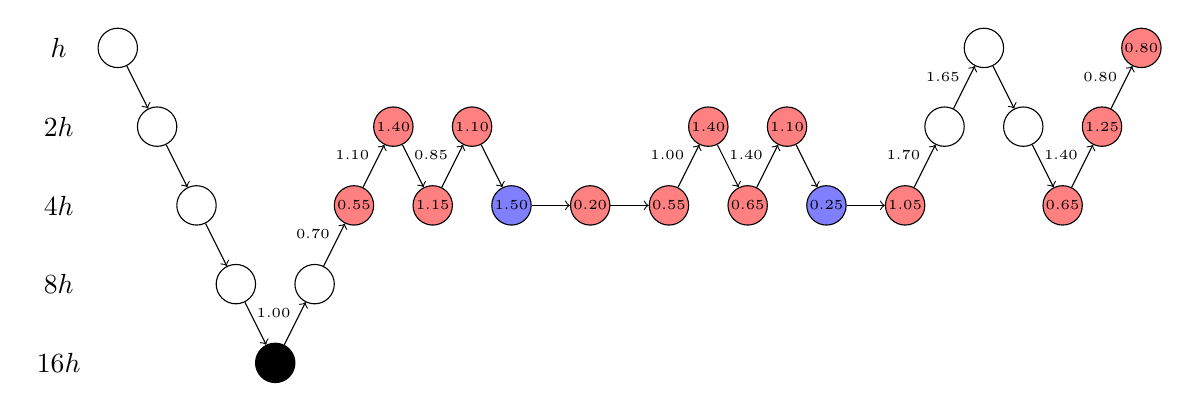
\begin{tikzpicture}
			\node   (h) at (-0.75, 4){$h$};
			\node   (2h) at (-0.75, 3){$2h$};
			\node   (4h) at (-0.75, 2){$4h$};
			\node   (8h) at (-0.75, 1){$8h$};
			\node   (16h) at (-0.75, 0){$16h$};
			\node	(a) at (0,4) [draw, circle,inner sep=0pt,minimum size=5mm] {\phantom{\tiny 1.00}};
			\node	(b) at (0.5,3) [draw, circle,inner sep=0pt,minimum size=5mm] {\phantom{\tiny 1.00}};
			\node	(c) at (1,2) [draw, circle,inner sep=0pt,minimum size=5mm] {\phantom{\tiny 1.00}};
			\node	(d) at (1.5,1) [draw, circle,inner sep=0pt,minimum size=5mm] {\phantom{\tiny 1.00}};
			\node	(e) at (2,0) [draw, circle,fill=black, inner sep=0pt,minimum size=5mm] {\phantom{\tiny 1.00}};
			\node	(f) at (2.5,1) [draw, circle,inner sep=0pt,minimum size=5mm] {\phantom{\tiny 1.00}};
			\node	(g) at (3,2) [draw, circle,fill=lightred,inner sep=0pt,minimum size=5mm] {\tiny 0.55};
			\node	(h) at (3.5,3) [draw, circle,fill=lightred,inner sep=0pt,minimum size=5mm] {\tiny 1.40};
			\node	(i) at (4,2) [draw, circle,fill=lightred,inner sep=0pt,minimum size=5mm] {\tiny 1.15};
			\node	(j) at (4.5,3) [draw, circle,fill=lightred, inner sep=0pt,minimum size=5mm] {\tiny 1.10};
			\node	(k) at (5,2) [draw, circle,fill=lightblue,inner sep=0pt,minimum size=5mm] {\tiny 1.50};
			\node	(l) at (6,2) [draw, circle,fill=lightred,inner sep=0pt,minimum size=5mm] {\tiny 0.20};
			\node	(m) at (7,2) [draw, circle, fill=lightred, inner sep=0pt,minimum size=5mm] {\tiny 0.55};
			\node	(n) at (7.5,3) [draw, circle,fill=lightred, inner sep=0pt,minimum size=5mm] {\tiny 1.40};
			\node	(o) at (8,2) [draw, circle, fill=lightred, inner sep=0pt,minimum size=5mm] {\tiny 0.65};
			\node	(p) at (8.5,3) [draw, circle,fill=lightred, inner sep=0pt,minimum size=5mm] {\tiny 1.10};
			\node	(q) at (9,2) [draw, circle, fill=lightblue, inner sep=0pt,minimum size=5mm] {\tiny 0.25};
			\node	(r) at (10,2) [draw, circle, fill=lightred, inner sep=0pt,minimum size=5mm] {\tiny 1.05};
			\node	(s) at (10.5,3) [draw, circle, inner sep=0pt,minimum size=5mm] {\phantom{\tiny 1.00}};
			\node	(t) at (11,4) [draw, circle, inner sep=0pt,minimum size=5mm] {\phantom{\tiny 1.00}};
			\node	(u) at (11.5,3) [draw, circle, inner sep=0pt,minimum size=5mm] {\phantom{\tiny 1.00}};
			\node	(v) at (12,2) [draw, circle, fill=lightred, inner sep=0pt,minimum size=5mm] {\tiny 0.65};
			\node	(w) at (12.5,3) [draw, circle, fill=lightred, inner sep=0pt,minimum size=5mm] {\tiny 1.25};
   			\node	(x) at (13,4) [draw, circle, fill=lightred, inner sep=0pt,minimum size=5mm] {\tiny 0.80};
			\draw 
			(a) edge[->] (b) 
			(b) edge[->] (c)
			(c) edge[->] (d)
			(d) edge[->] (e)   
			(e) edge[->] node[near end,left] {\tiny 1.00} (f)
			(f) edge[->] node[near end,left] {\tiny 0.70} (g)
			(g) edge[->] node[near end,left] {\tiny 1.10} (h)
			(h) edge[->] (i)
			(i) edge[->] node[near end,left] {\tiny 0.85} (j) 
			(j) edge[->] (k)
			(k) edge[->] (l)
			(l) edge[->] (m)   
			(m) edge[->] node[near end,left] {\tiny 1.00} (n)
			(n) edge[->] (o)
			(o) edge[->] node[near end,left] {\tiny 1.40} (p)
			(p) edge[->] (q)
			(q) edge[->] (r)
			(r) edge[->] node[near end,left] {\tiny 1.70} (s)
			(s) edge[->] node[near end,left] {\tiny 1.65} (t)
			(t) edge[->] (u)
			(u) edge[->] (v)
			(v) edge[->] node[near end,left] {\tiny 1.40} (w)
   			(w) edge[->] node[near end,left] {\tiny 0.80} (x)
			;
			\end{tikzpicture}
		}
		\caption{EP-10}
		\label{fig:ep-10}
	\end{subfigure}
	\caption{Computational structure of the evolved multigrid preconditioners. The color of the node denotes the type of operation. Black: Coarse-grid solver, Blue: Pointwise Jacobi smoothing, Red: Red-black Gauss-Seidel smoothing, White: No operation. The relaxation factor of each smoothing step is included in each node, while for coarse-grid correction, it is attached to the respective edge.}
	\label{fig:structure-evolved-preconditioners}
\end{figure}
First of all, both multigrid methods employ a unique sequence of operations that does not resemble any known multigrid cycle.
While both methods initially apply the coarse-grid solver exactly once and, thus, resemble a V-cycle, they incorporate additional smoothing-based coarse-grid correction steps.
Furthermore, our grammar-based representation enables the combination of different smoothers or even the complete omission of smoothing on certain levels.
While both methods employ predominantly red-black Gauss-Seidel smoothing, especially EP-2 also incorporates multiple intermediate Jacobi steps.
With respect to the number of smoothing steps, similar to the most efficient reference methods, V(0,1), V(1,1), and F(0,1), smoothing on the finest grid is reduced to a bare minimum, in the form of one or two red-black Gauss-Seidel steps.
However, this is augmented with a significantly larger number of smoothing and coarse-grid correction steps on subsequent levels, which is in contrast to the uniform structure of classical multigrid cycles.
In general, the computational structure of EP-2 comprises a higher degree of regularity since, at its end,
the same sequence of operations is repeated three times.
While within each execution of this sequence, the relaxation factors of certain smoothing operations are altered, the same two values, 0.30 and 0.85, are employed within the two coarse-grid correction steps.
The computational structure of EP-5 is less uniform compared to EP-2.
However, on the second finest grid, the method repeatedly applies a similar sequence of restriction, smoothing, and prolongation, whereby in each step, a different combination of smoothers is used.
The resulting effectiveness of both multigrid methods as a preconditioner, together with their high computational efficiency, highlights the advantages of our grammar-based representation.
The construction of both methods requires the alternation of individual operations within their sequence.
Encoding the computational structure of a multigrid method based on a number of global parameters does not come with that flexibility.
For instance, choosing a different value for $\mu$ in Algorithm~\ref{alg:multigrid-cycle} changes the number of recursive descents on each level of the method.
However, none of the available parameters offers a way to insert a single coarse-grid correction or smoothing step after at a specific position within the sequence.
In contrast, expressing each computational step in the form of a separate production within a formal grammar allows us to achieve this goal by inserting the corresponding subtree into the respective derivation tree, as discussed in Section~\ref{sec:gggp} and Chapter~\ref{chapter:multigrid-formal-language}.

Finally, we need to address the question of why our evolutionary program synthesis did not consistently discover multigrid-based preconditioners that achieve the same degree of efficiency and generalizability in each experiment.
For this purpose, we again consider the space of non-dominated solutions at the end of each experiment, which is shown in Figure~\ref{fig:pareto-front-helmholtz}.
\begin{figure}
	\includegraphics[width=\textwidth]{figures/pareto-front.pdf}
	\caption{Distribution of non-dominated solutions at the end of all ten experiments for $k = 320$. The red line denotes the combined front.}
	\label{fig:pareto-front-helmholtz}
\end{figure}
First of all, note that the number of non-dominated solutions is smaller than in the experiments performed in Section~\ref{sec:experiments-part1}.
However, this is clearly expected due to the smaller population size, which is only half as large as in our previous experiments.
Furthermore, as we iteratively increase the problem size and difficulty, the algorithm is forced to adapt the current population to the new characteristics of the problem within only 50 generations, which increases the difficulty of evolving the same number of non-dominated individuals. 
However, despite this fact, our evolutionary algorithm achieves a high degree of consistency in finding individuals that are located on the right half of the objective function space.
In contrast, in the left half of Figure~\ref{fig:pareto-front-helmholtz}, which corresponds to those individuals that lead to increasingly effective but more costly preconditioners, the algorithm is not able to find the same non-dominated individuals in each experiment.
Note that all multigrid-based preconditioners considered in our final evaluation shown in Table~\ref{table:evolved-solvers} correspond to individuals located here.
The larger distance of certain individuals in Figure~\ref{fig:pareto-front-helmholtz} to the combined front, therefore, explains why we could not achieve the same degree of efficiency in each run.
To reduce the number of iterations until convergence through preconditioning, we need to improve the accuracy of the approximate solution computed for Equation~\eqref{eq:helmholtz-test-problem-preconditioning}.
Since this requires us to perform more smoothing and coarse-grid correction steps, the size of the corresponding derivation trees grows accordingly.
In order to obtain the same derivation tree, we need to find an exact sequence of productions starting from a random initialization in each individual run of our algorithm.
As we have already investigated in Section~\ref{sec:experiments1-algorithm-behavior-analysis}, NSGA-II struggles to achieve this goal consistently~\cite{liu2022evolvability}, which, in certain experiments, leads to a suboptimal outcome in the leftmost part of the objective function space.

\chapter{Comparison with Related Work}
\chapter{Conclusion}

% start the appendix (arabic page numbering [continued],
% uppercase alphabetic sectioning numbering, header)
\appendix 
  
  %%% WRITE YOUR APPENDIX DIRECTLY HERE OR %%%%%%%%
  %%% INPUT AN EXTERNAL FILE WITH YOUR APPENDIX %%%
  \section{Intermediate Representation}
\label{appendix:ir}
\begin{listing}[!htb]
	\inputminted{python}{evostencils/ir/inter_grid_operator.py}
	\caption{IR: Inter-Grid Operator Base Class}
	\label{code:ir:inter-grid-operator}
\end{listing}
\begin{listing}[!htb]
	\inputminted{python}{evostencils/ir/restriction.py}
	\caption{IR: Restriction}
	\label{code:ir:restriction}
\end{listing}
\begin{listing}[!htb]
	\inputminted{python}{evostencils/ir/prolongation.py}
	\caption{IR: Prolongation}
	\label{code:ir:prolongation}
\end{listing}
\begin{listing}[!htb]
	\inputminted{python}{evostencils/ir/diagonal.py}
	\caption{IR: Diagonal and Block-Diagonal}
	\label{code:ir:diagonal}
\end{listing}
\begin{listing}[!htb]
	\inputminted{python}{evostencils/ir/multiplication.py}
	\caption{IR: Operator Application}
	\label{code:ir:multiplication}
\end{listing}
\begin{listing}[!htb]
	\inputminted{python}{evostencils/ir/coarse_grid_solver.py}
	\caption{IR: Coarse-Grid Solver}
	\label{code:ir:coarse-grid-solver}
\end{listing}
\clearpage
\section{Genetic Programming}
\label{appendix:gp}
\begin{listing}[!htb]
	\inputminted{python}{evostencils/gp/primitive_set_typed.py}
	\caption{PrimitiveSetTyped}
	\label{code:gp:primitive-set-typed}
\end{listing}
\begin{listing}[!htb]
	\inputminted{python}{evostencils/gp/generate.py}
	\caption{Tree generation function}
	\label{code:gp:generate}
\end{listing}

    
% start the backmatter (arabic page numbering [continued],
% no sectioning numbering, header)
\backmatter
  \faupressprintbibliography

\end{document}
